\bibliography{../References/refer}

\section{Experiment}
	\label{sec:Experiment}
	\subsection{Overview}
	The experiments consisted of generating lists of integers ranging in size from four to fifty million. The integers were chosen uniformly at random between zero and $10^{12}$. Consecutive lists were $9/7$ the size of the previous rounded down to the nearest integer. Each quicksort and each of it's variations sorted the same list. The number of comparisons, swaps and time taken by each quicksort were recorded. A summary of the conditions can be found in Table \ref{tab:experimentConditions} for a total of 17 conditions. A total of 69 iterations were run resulting in 109296 data points. During each iteration, the data gathering for each list size was done in parallel using four threads.

	\begin{table}
		\begin{center}
			\begin{tabular}{|r|c|c|c}
				\hline
				Sort           			&  Pivot Selection methods 	& Number of Pivots 	\\ \hline \hline
				Classic                 &  3 						& 1       			\\ \hline
				Dual Pivot              &  2  						& 2       			\\ \hline
				Optimal Dual Pivot      &  2  						& 2       			\\ \hline
				Yaroslavskiy            &  1  						& 2       			\\ \hline
				Three Pivot             &  1  						& 3       			\\ \hline
				M-Pivot                 &  1  						& 3,4,5,6 			\\ \hline
				Heap Optimized M-Pivot  &  1  						& 3,4,5,6 			\\ \hline
			\end{tabular}
			\caption{List of all the variation of quicksorts executed.}
			\label{tab:experimentConditions}
		\end{center}
	\end{table}


	\subsection{Platform}
	The experiments were run on a virtual machine with OSX 10.9 as the guest operating system and Windows 8.1 as the host operating system. The host operating system has 16 GB of ram and an i5-2500k CPU overclocked to 4.3 GHz. The guest OS had access to 8 GB of RAM and access to all 4 cores of the host CPU.

	\subsection{Results}
	%**********************************************************************
	% Determine if we need to talk about pivot selection here
	%**********************************************************************
	%The pivot selection methods differ by which quicksort algorithm we are referring too.
	%For the classic quick sort algorithm, 
	%the pivot selection method $1$ and $2$ would refer to picking the first or last element as the pivot respectively.
	%Pivot selection method $3$ refers to picking the median of 3 elements.
	%Which these would be the one of the first, middle, or last element.
	%For dual pivot and optimal dual pivot, pivot selection $1$ refers
	\begin{figure}[ht!]
		\begin{center}   
			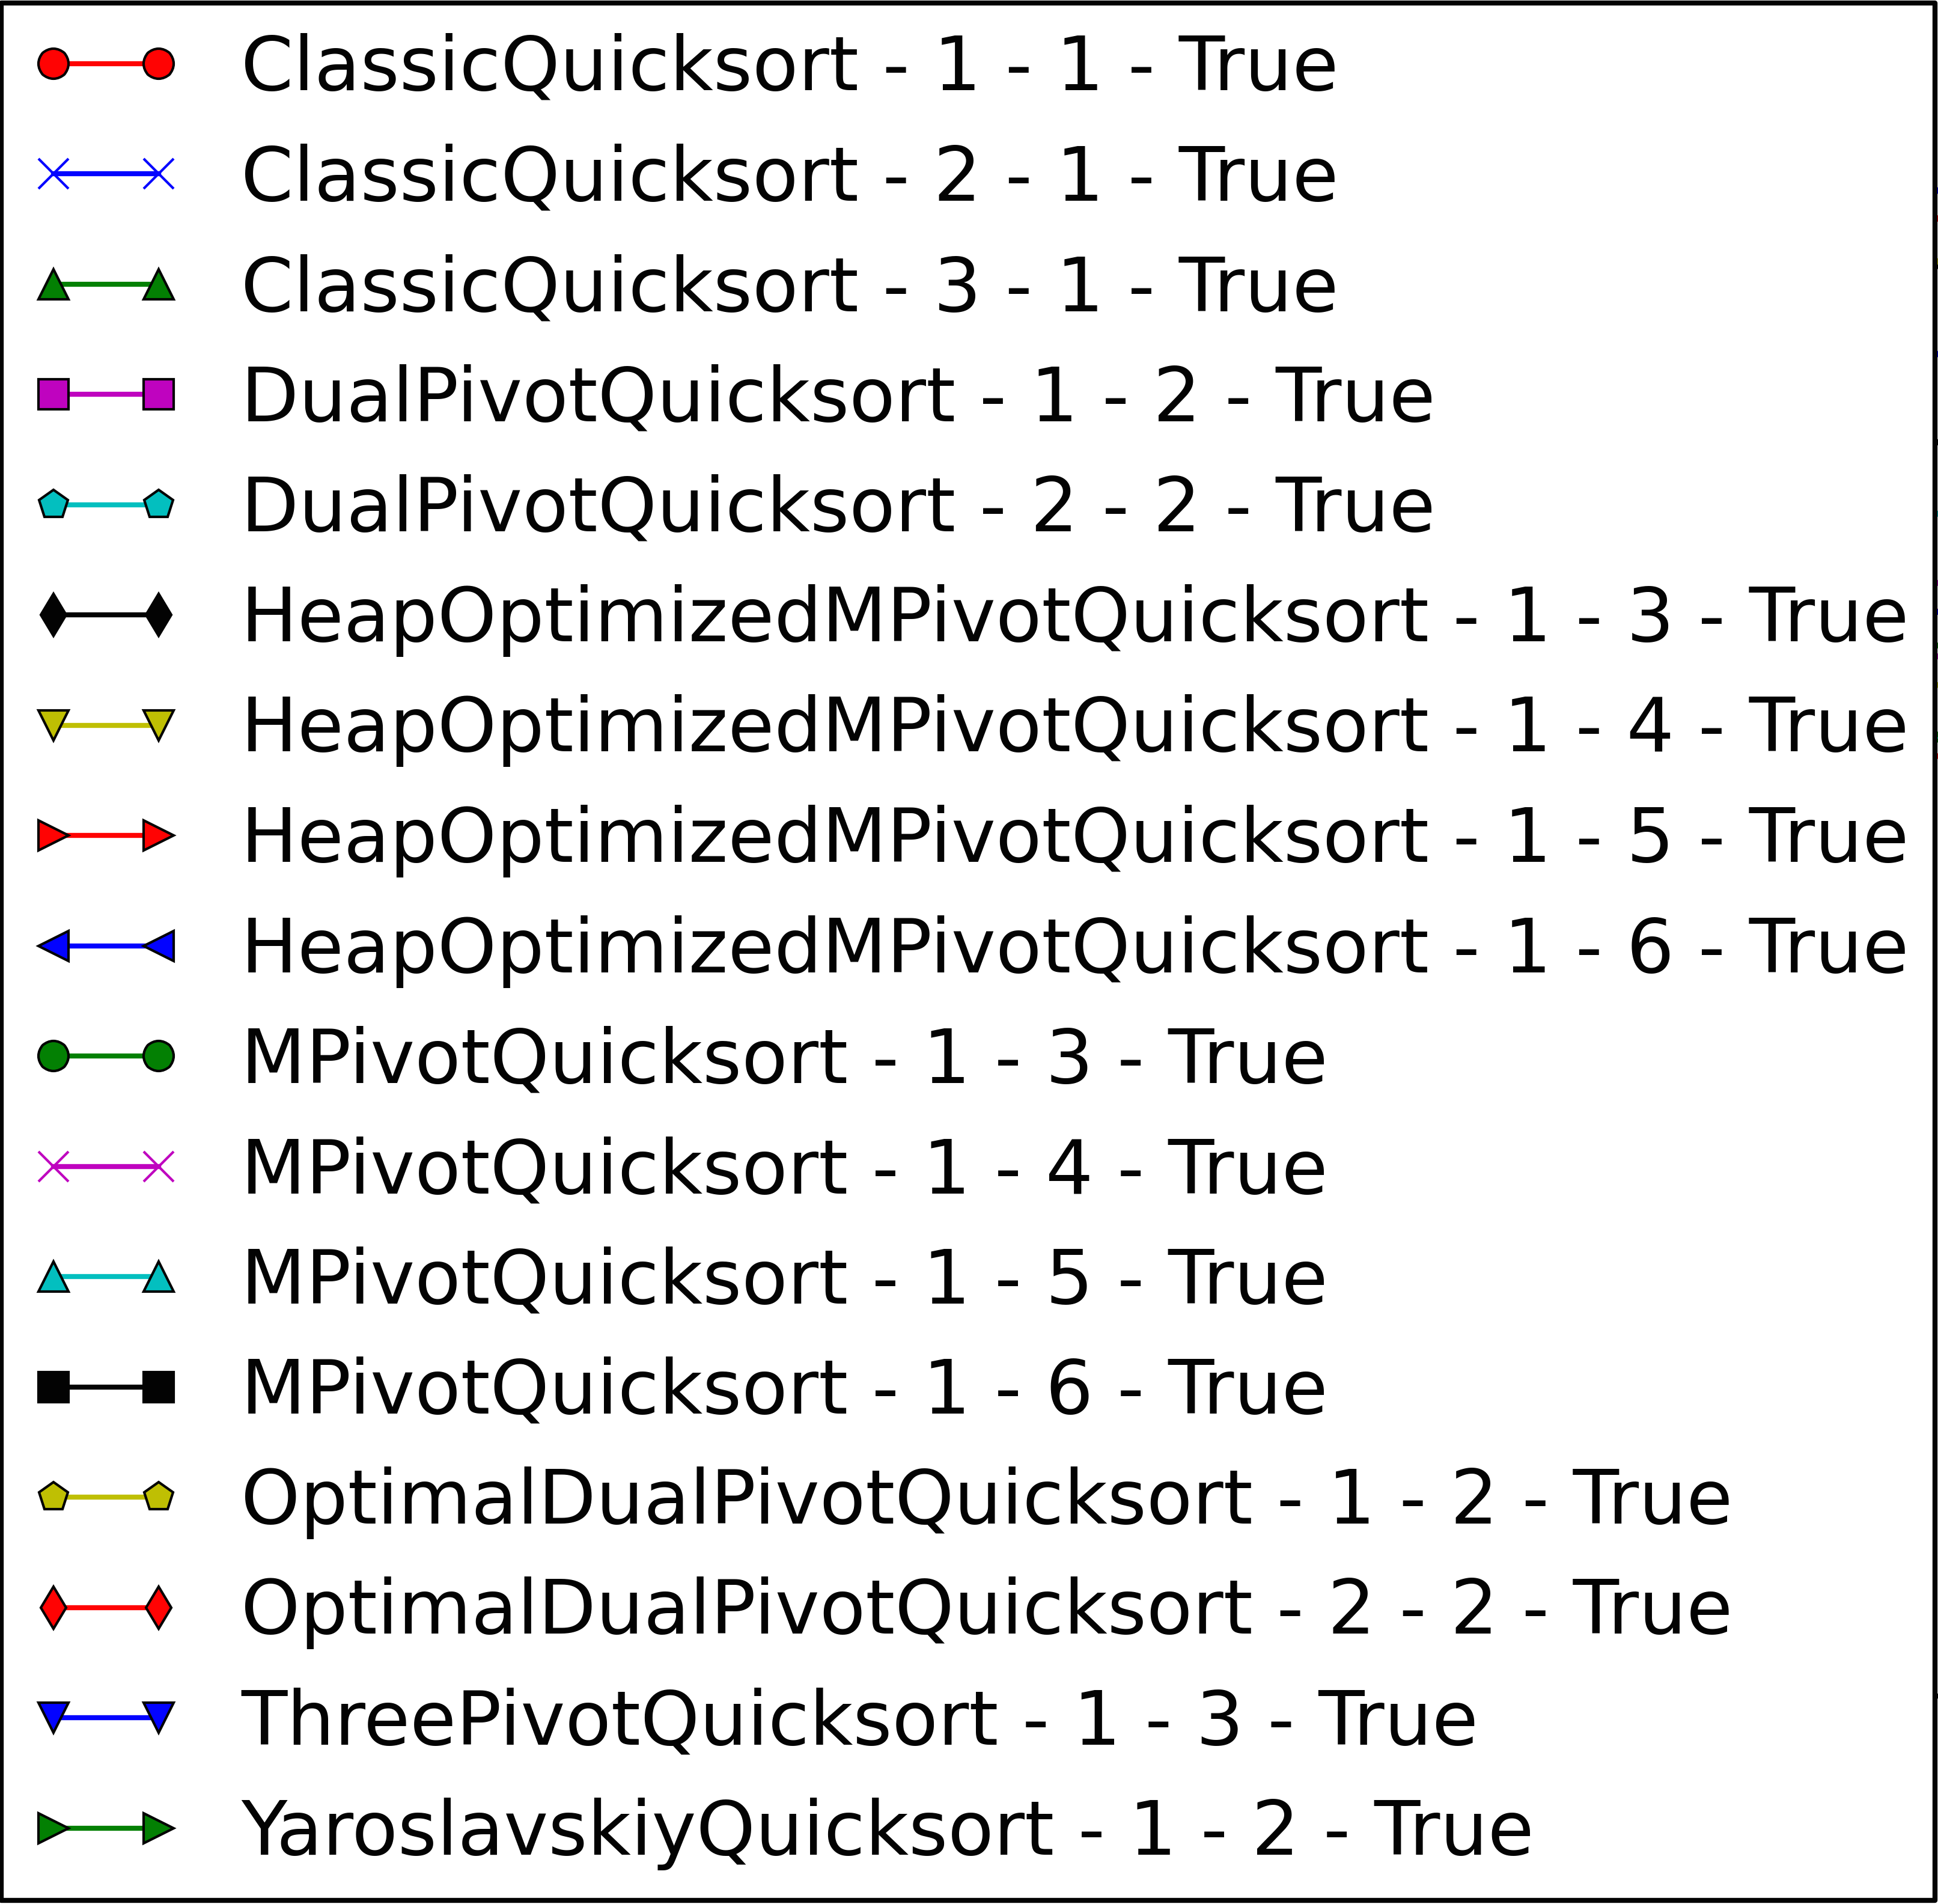
\includegraphics[width=85mm]{PlotLegend.png}
			\caption{Plot legend}
			\label{fig:PlotLegend}
		\end{center}
	\end{figure}

	%**********************************************************************
	% All Plots Large Scale
	%**********************************************************************
	\begin{figure}[ht!]
		\begin{center}
			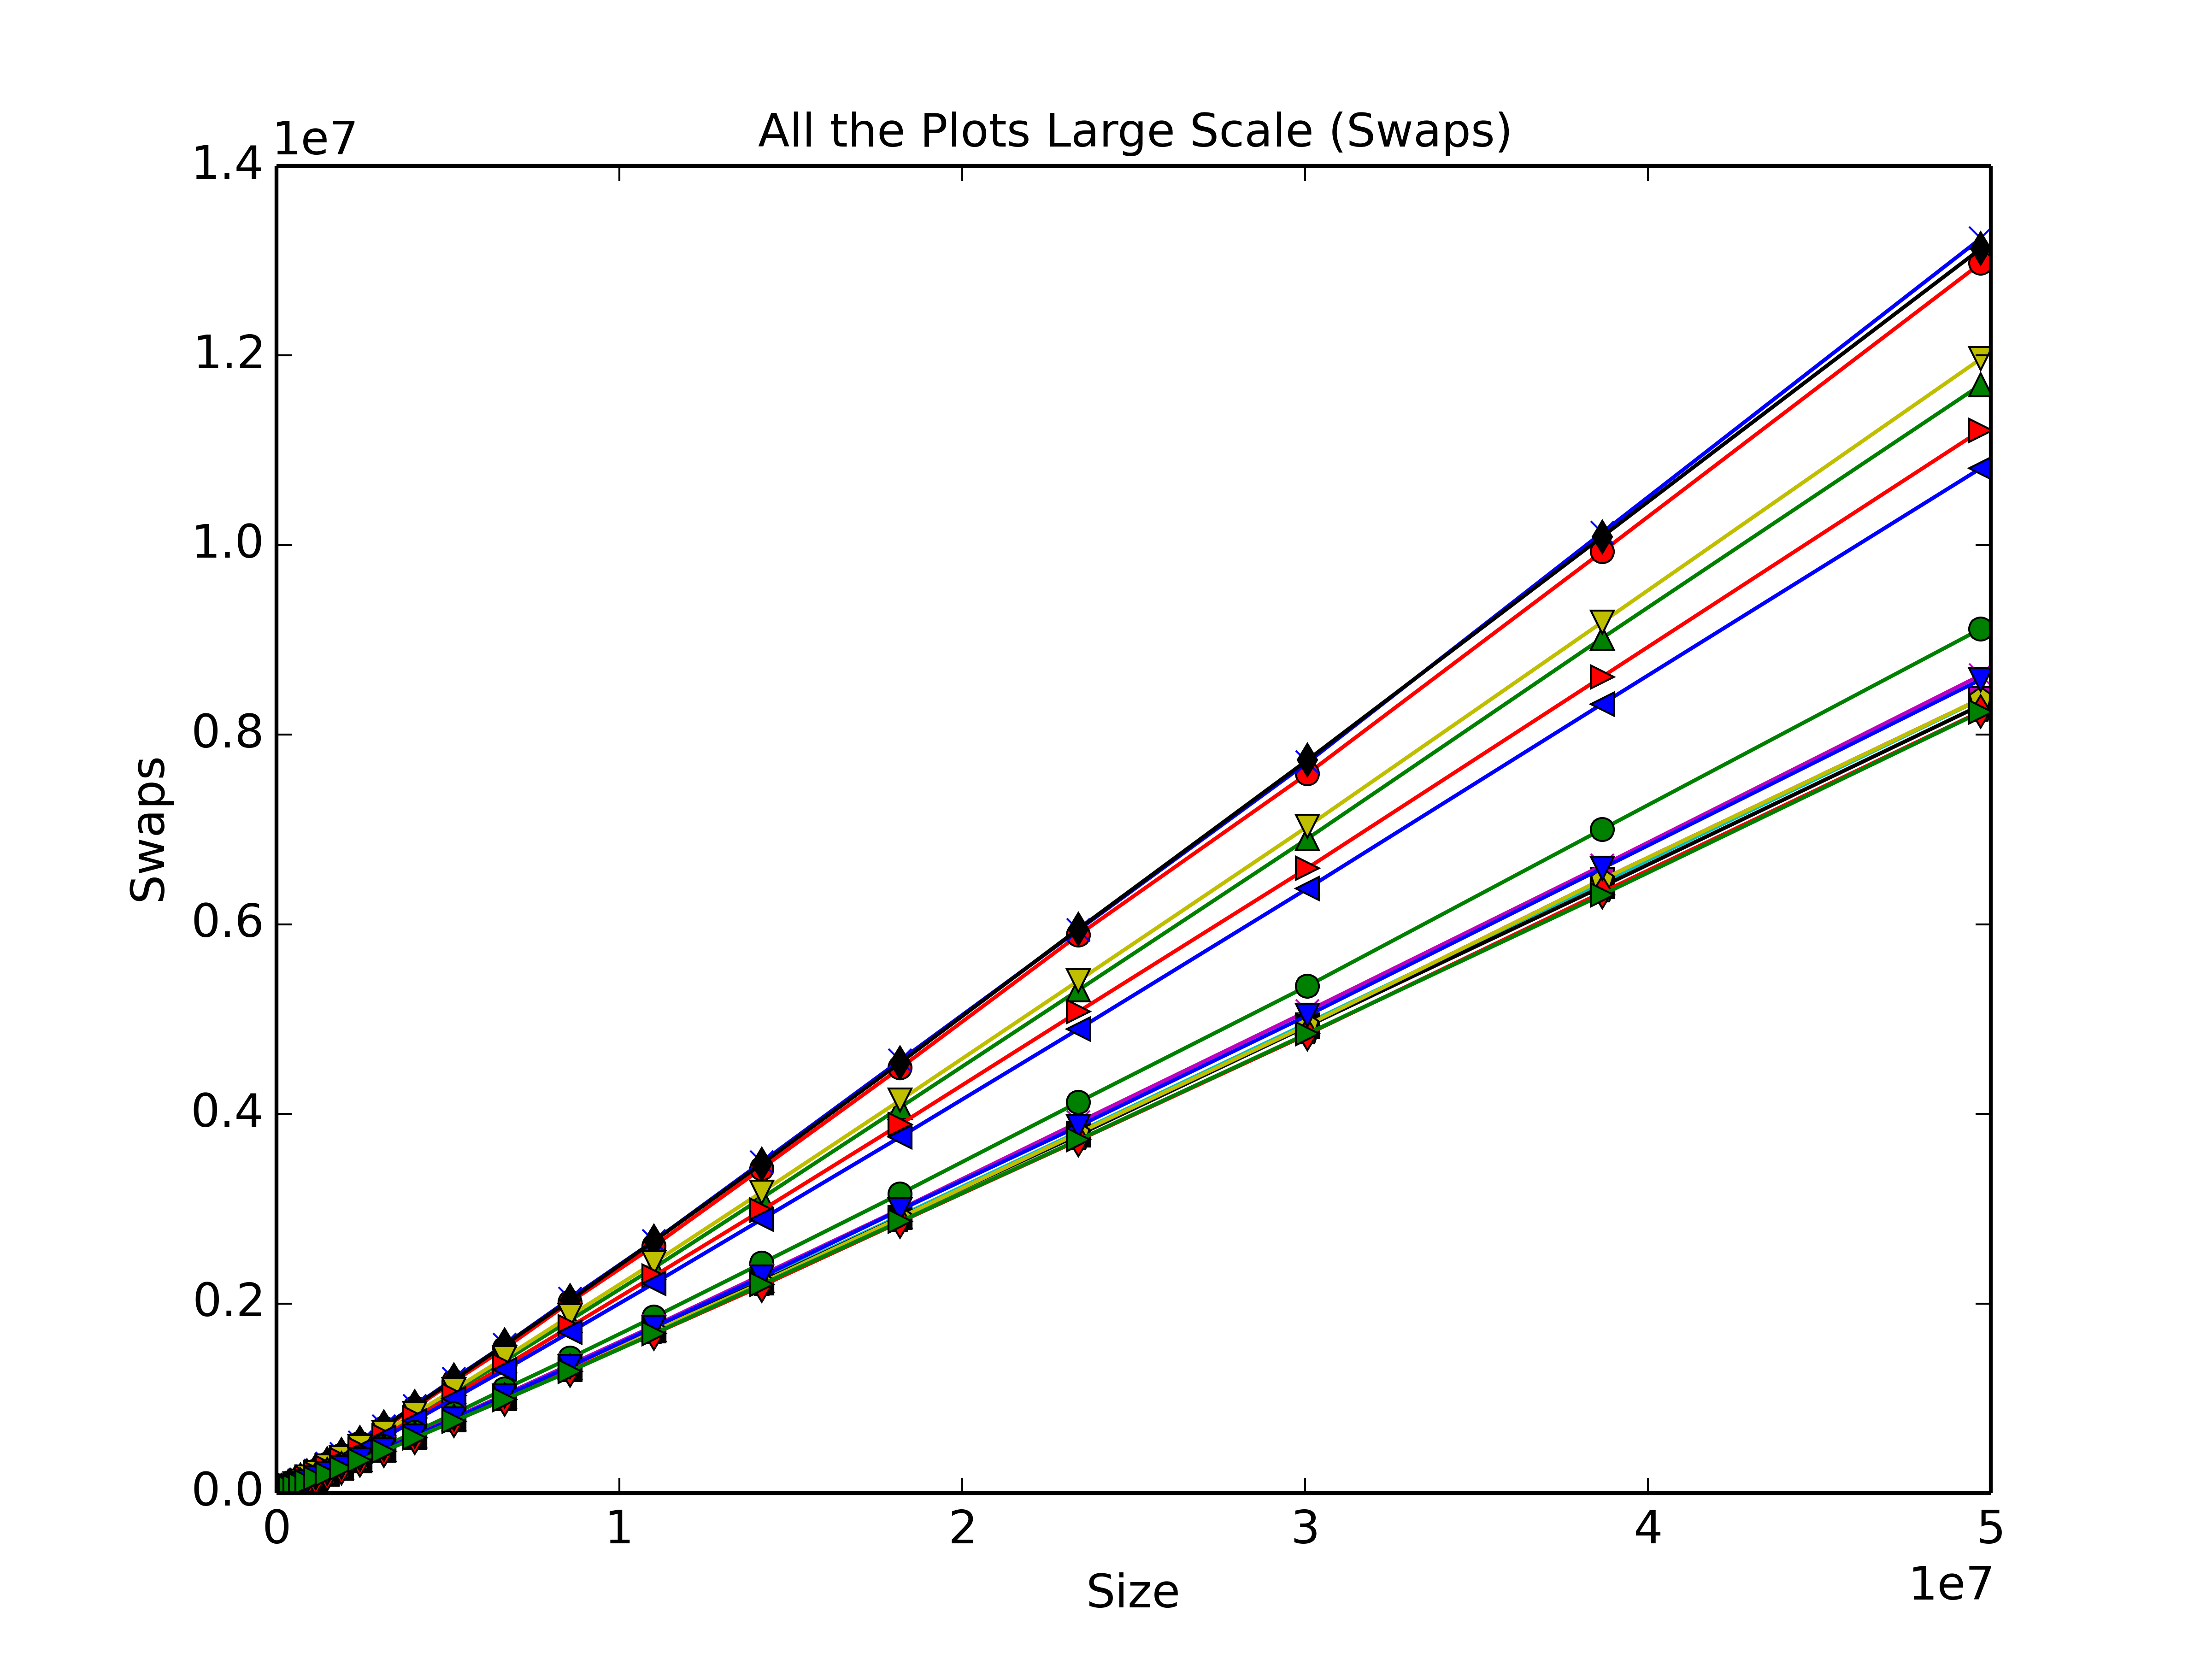
\includegraphics[width=120mm]{AllthePlotsLargeScale_swap}
			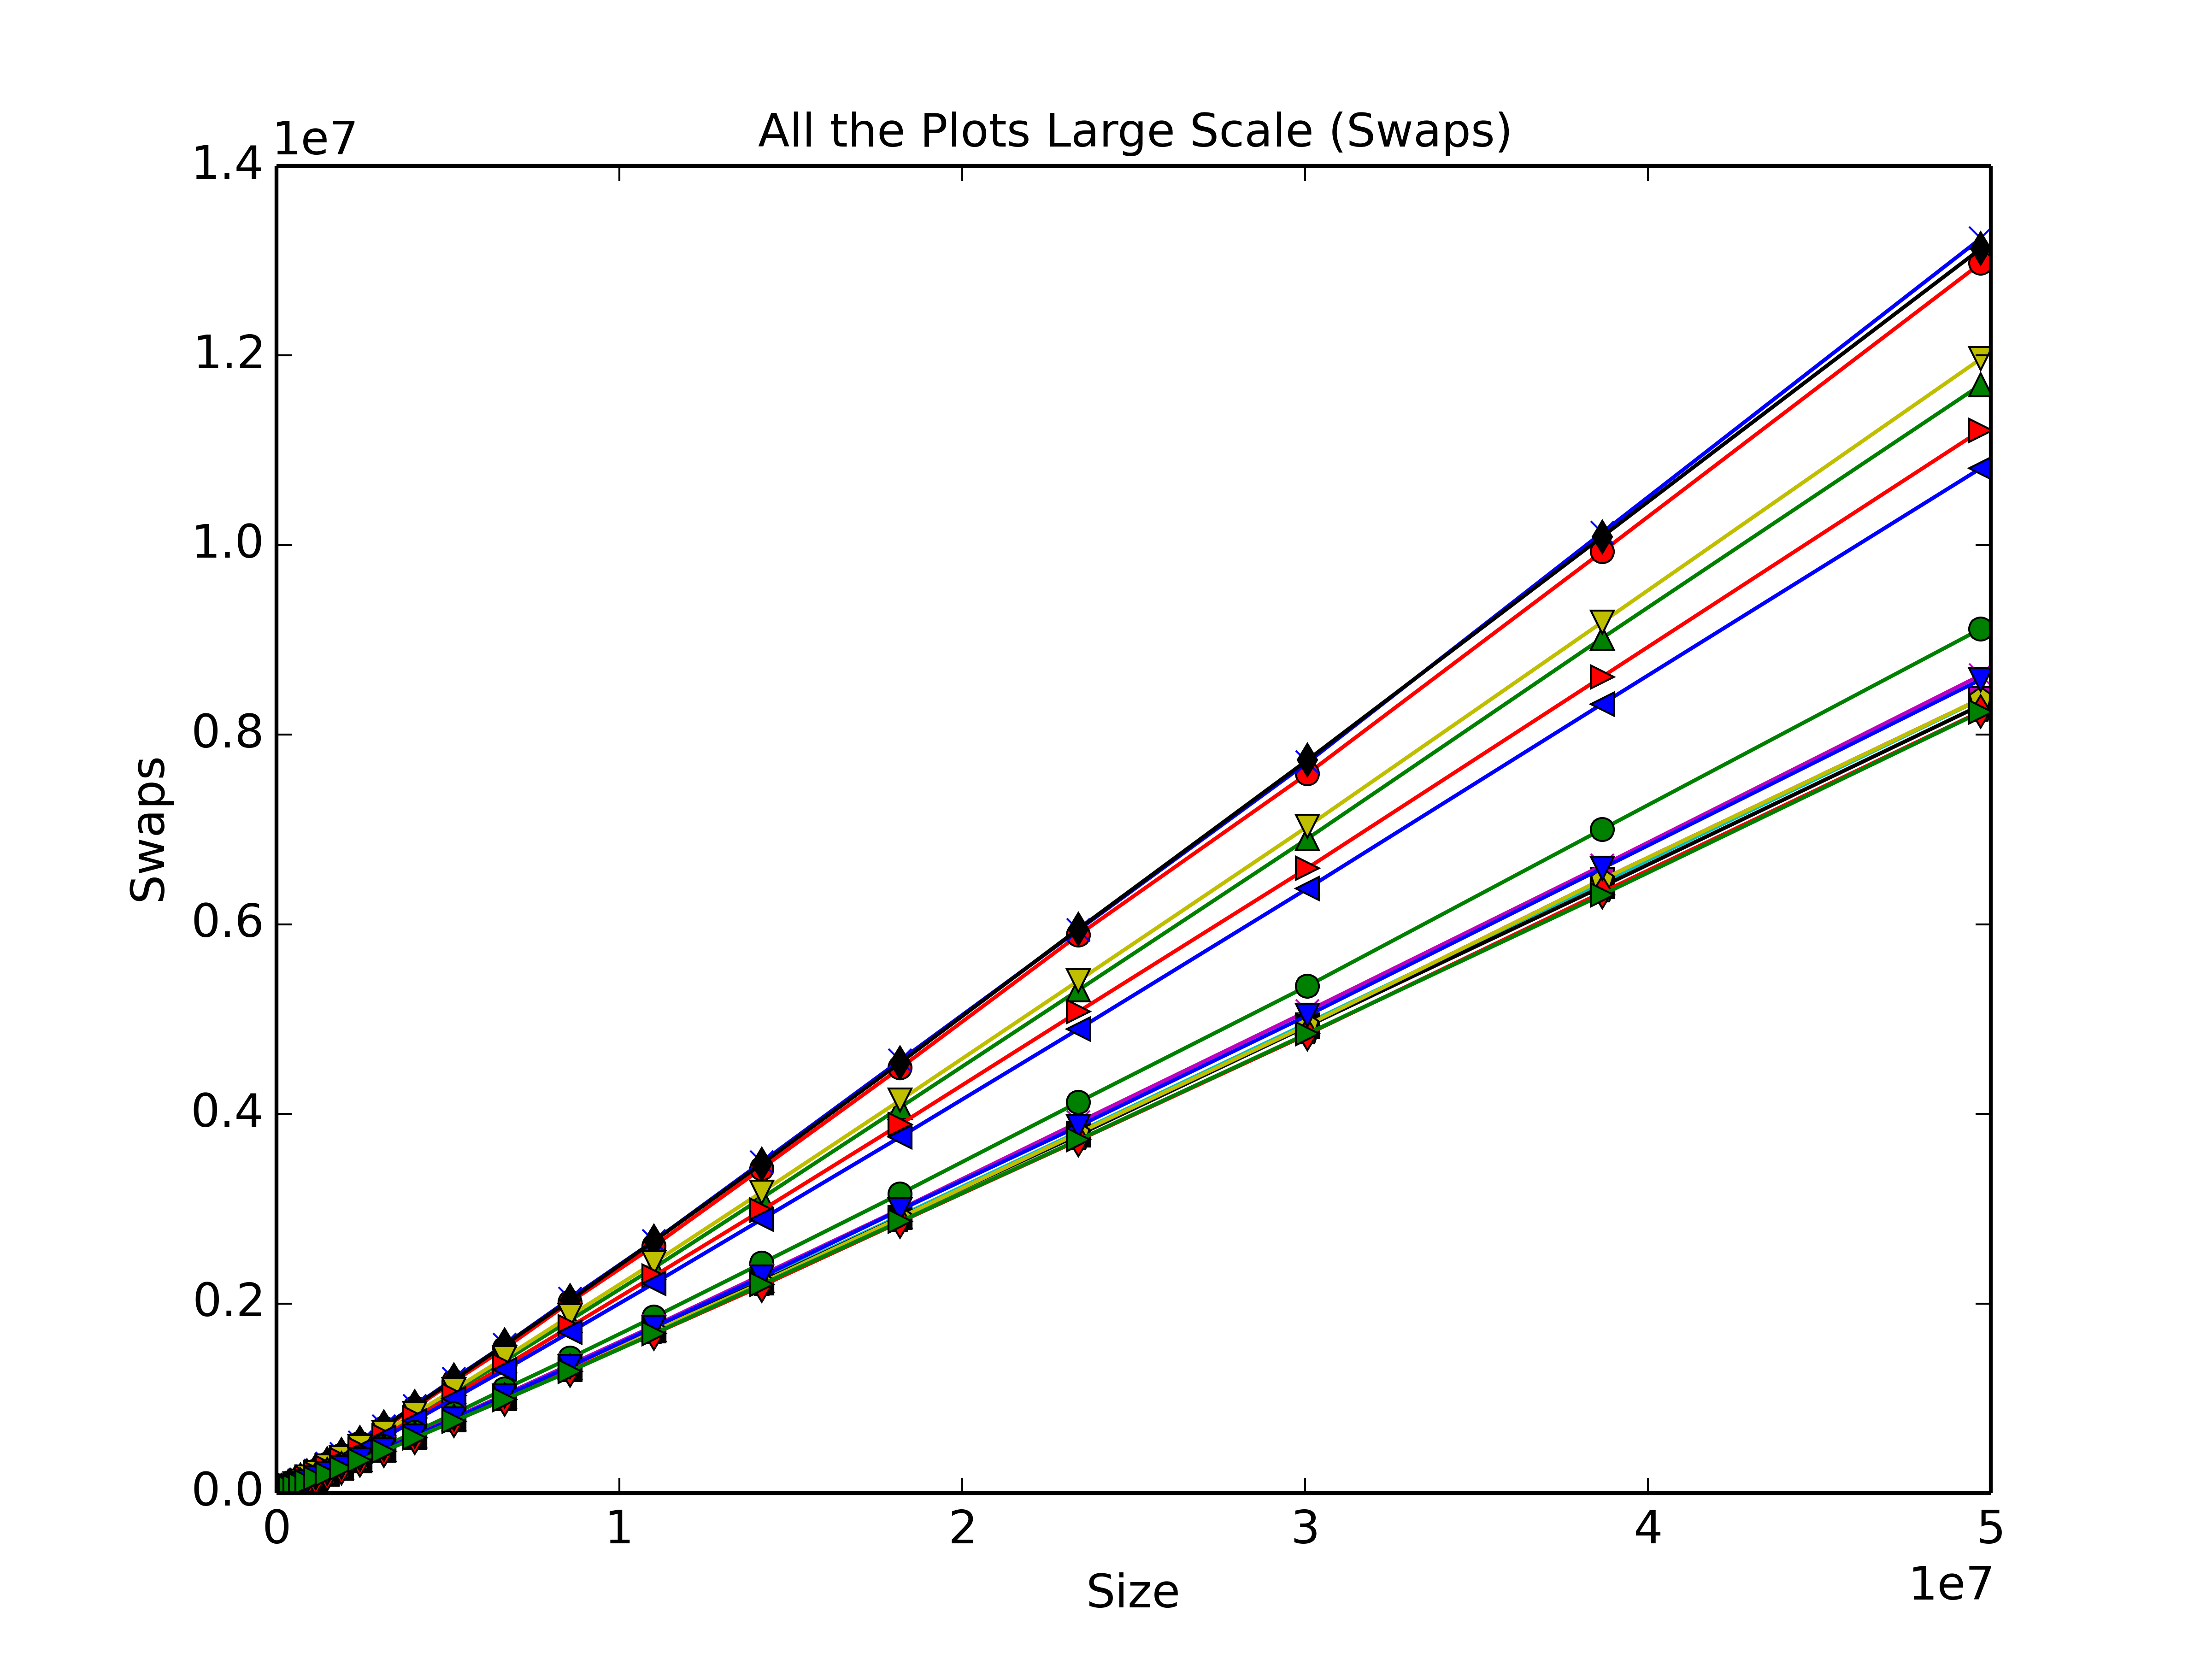
\includegraphics[width=120mm]{AllthePlotsLargeScale_swap}
			\caption{A plot of the data from all the sorting algorithm against the number of comparisons.}
			\label{fig:AllSorts}
		\end{center}
	\end{figure}


	%**********************************************************************
	% All Plots Log Large Scale
	%**********************************************************************
	\begin{figure}[ht!]
		\begin{center}
			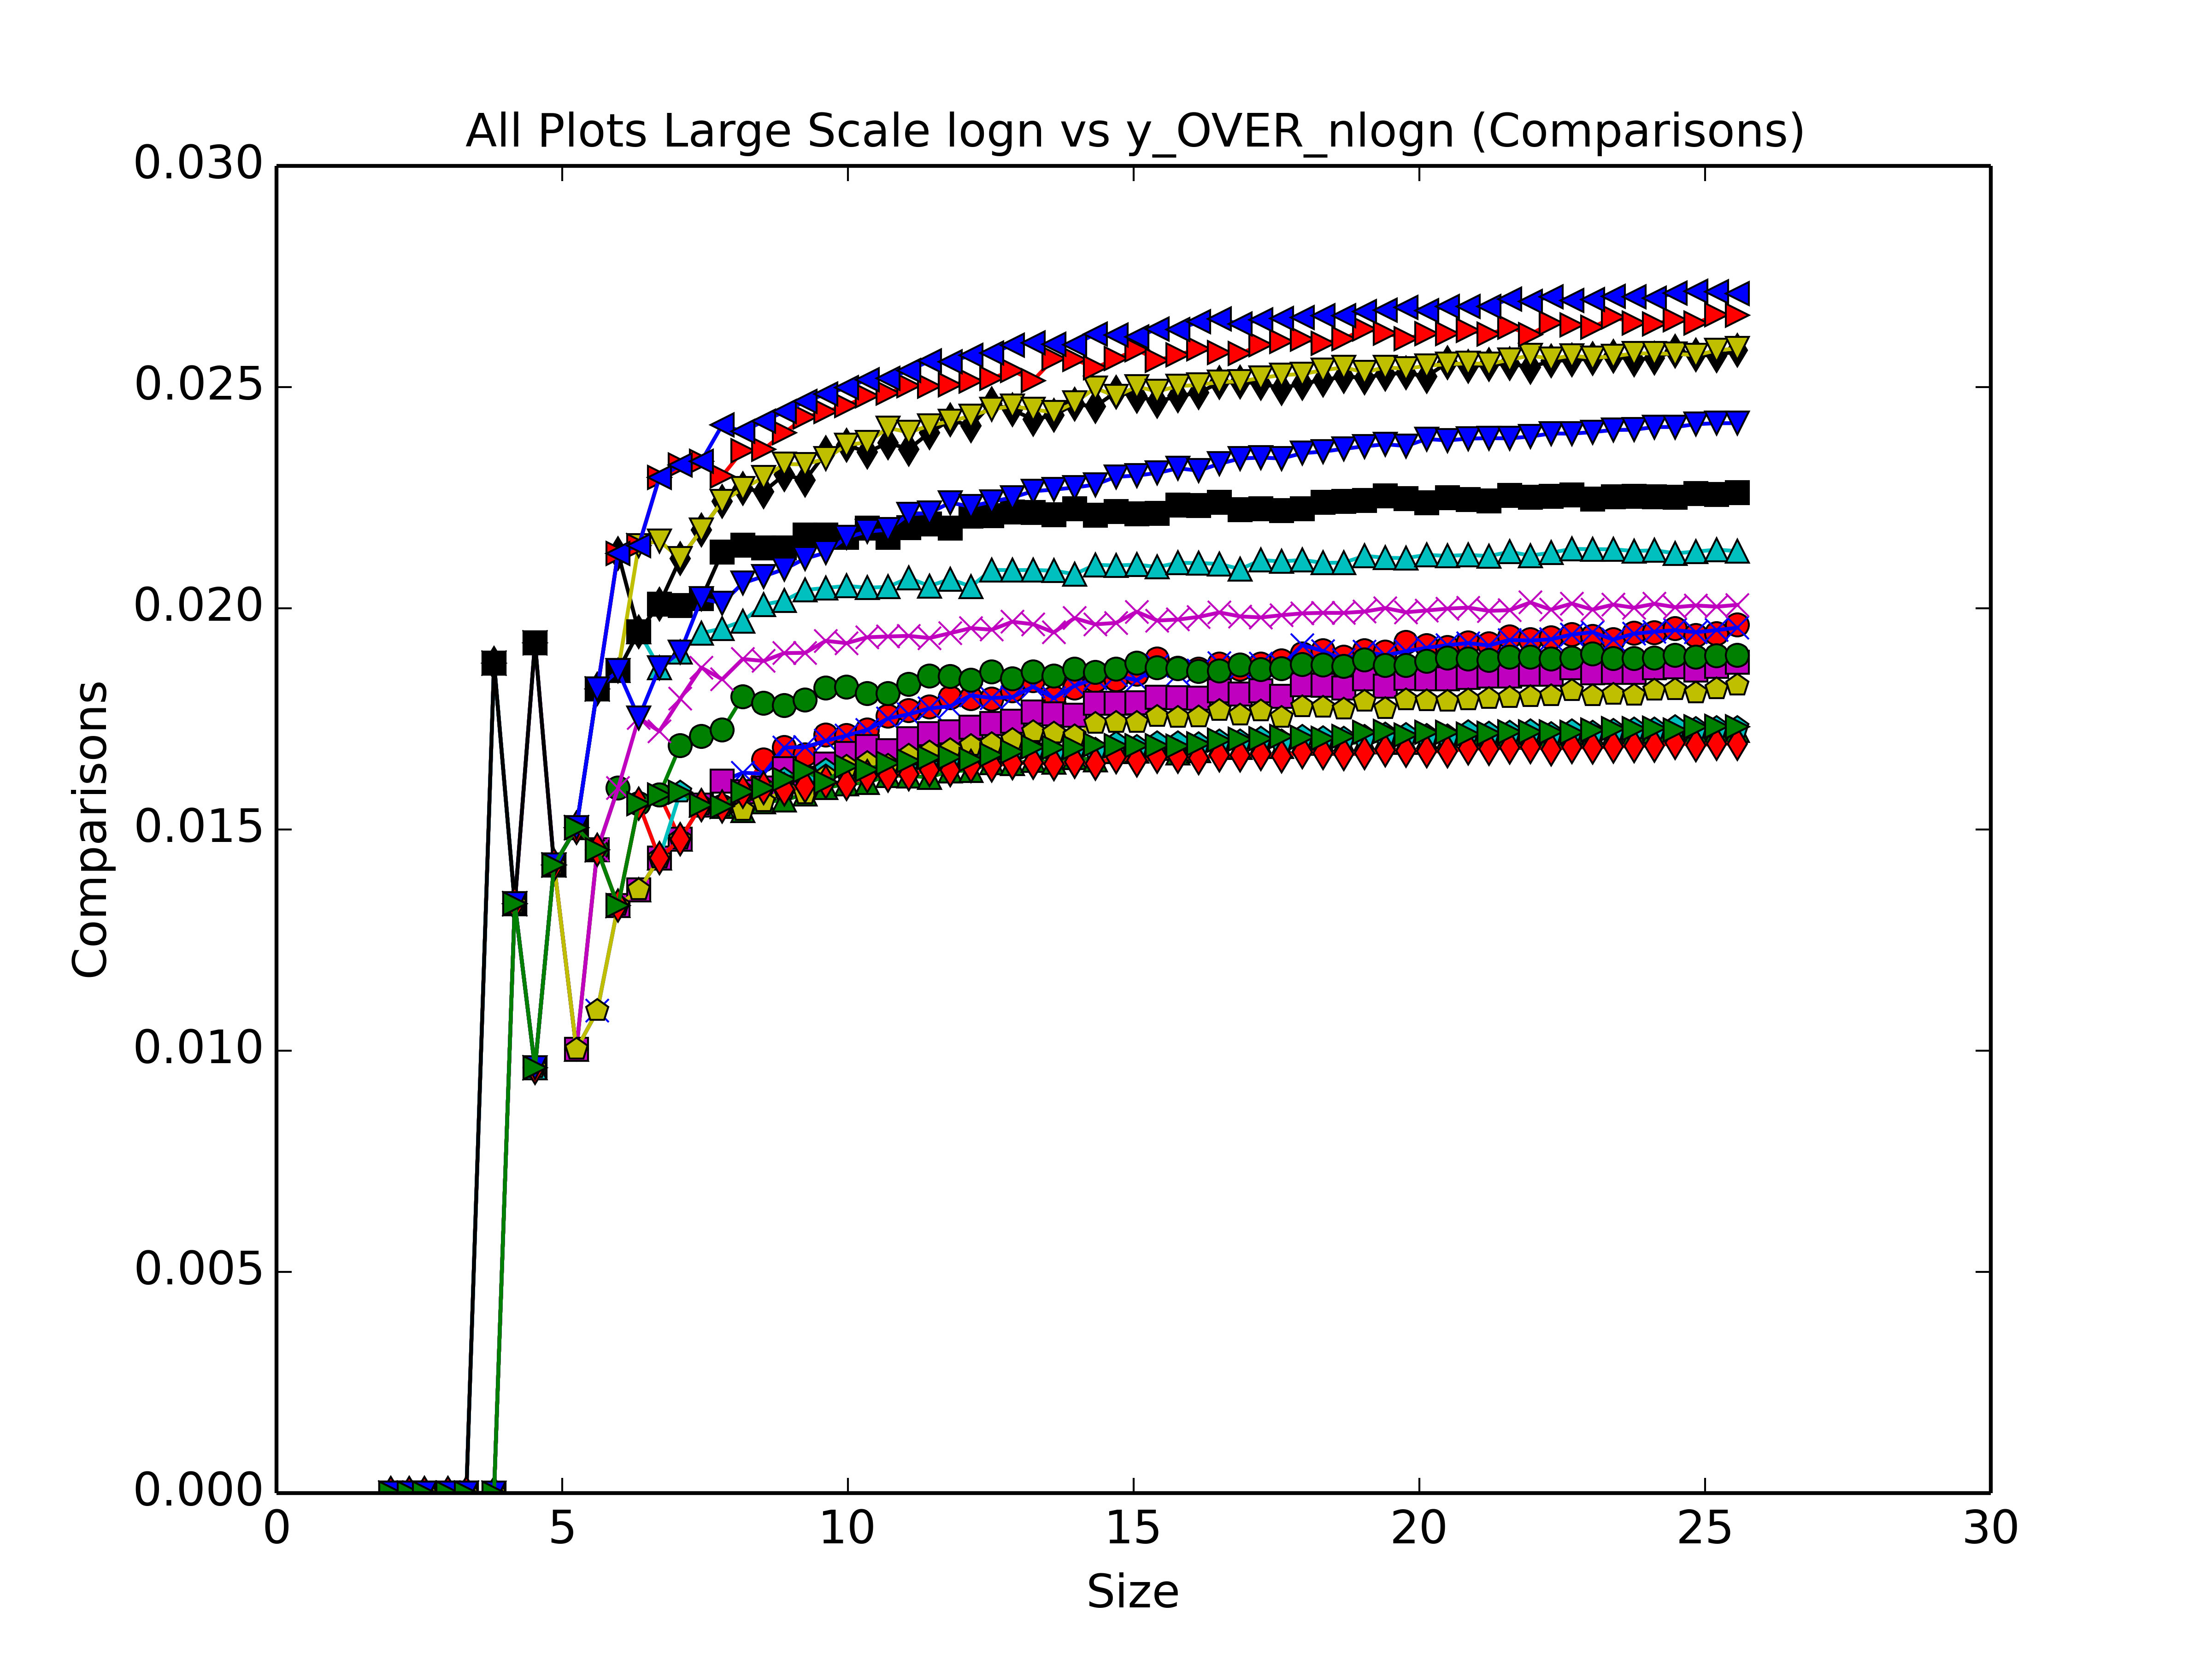
\includegraphics[width=120mm]{AllPlotsLargeScalelognvsy_OVER_nlogn_comp.png}
			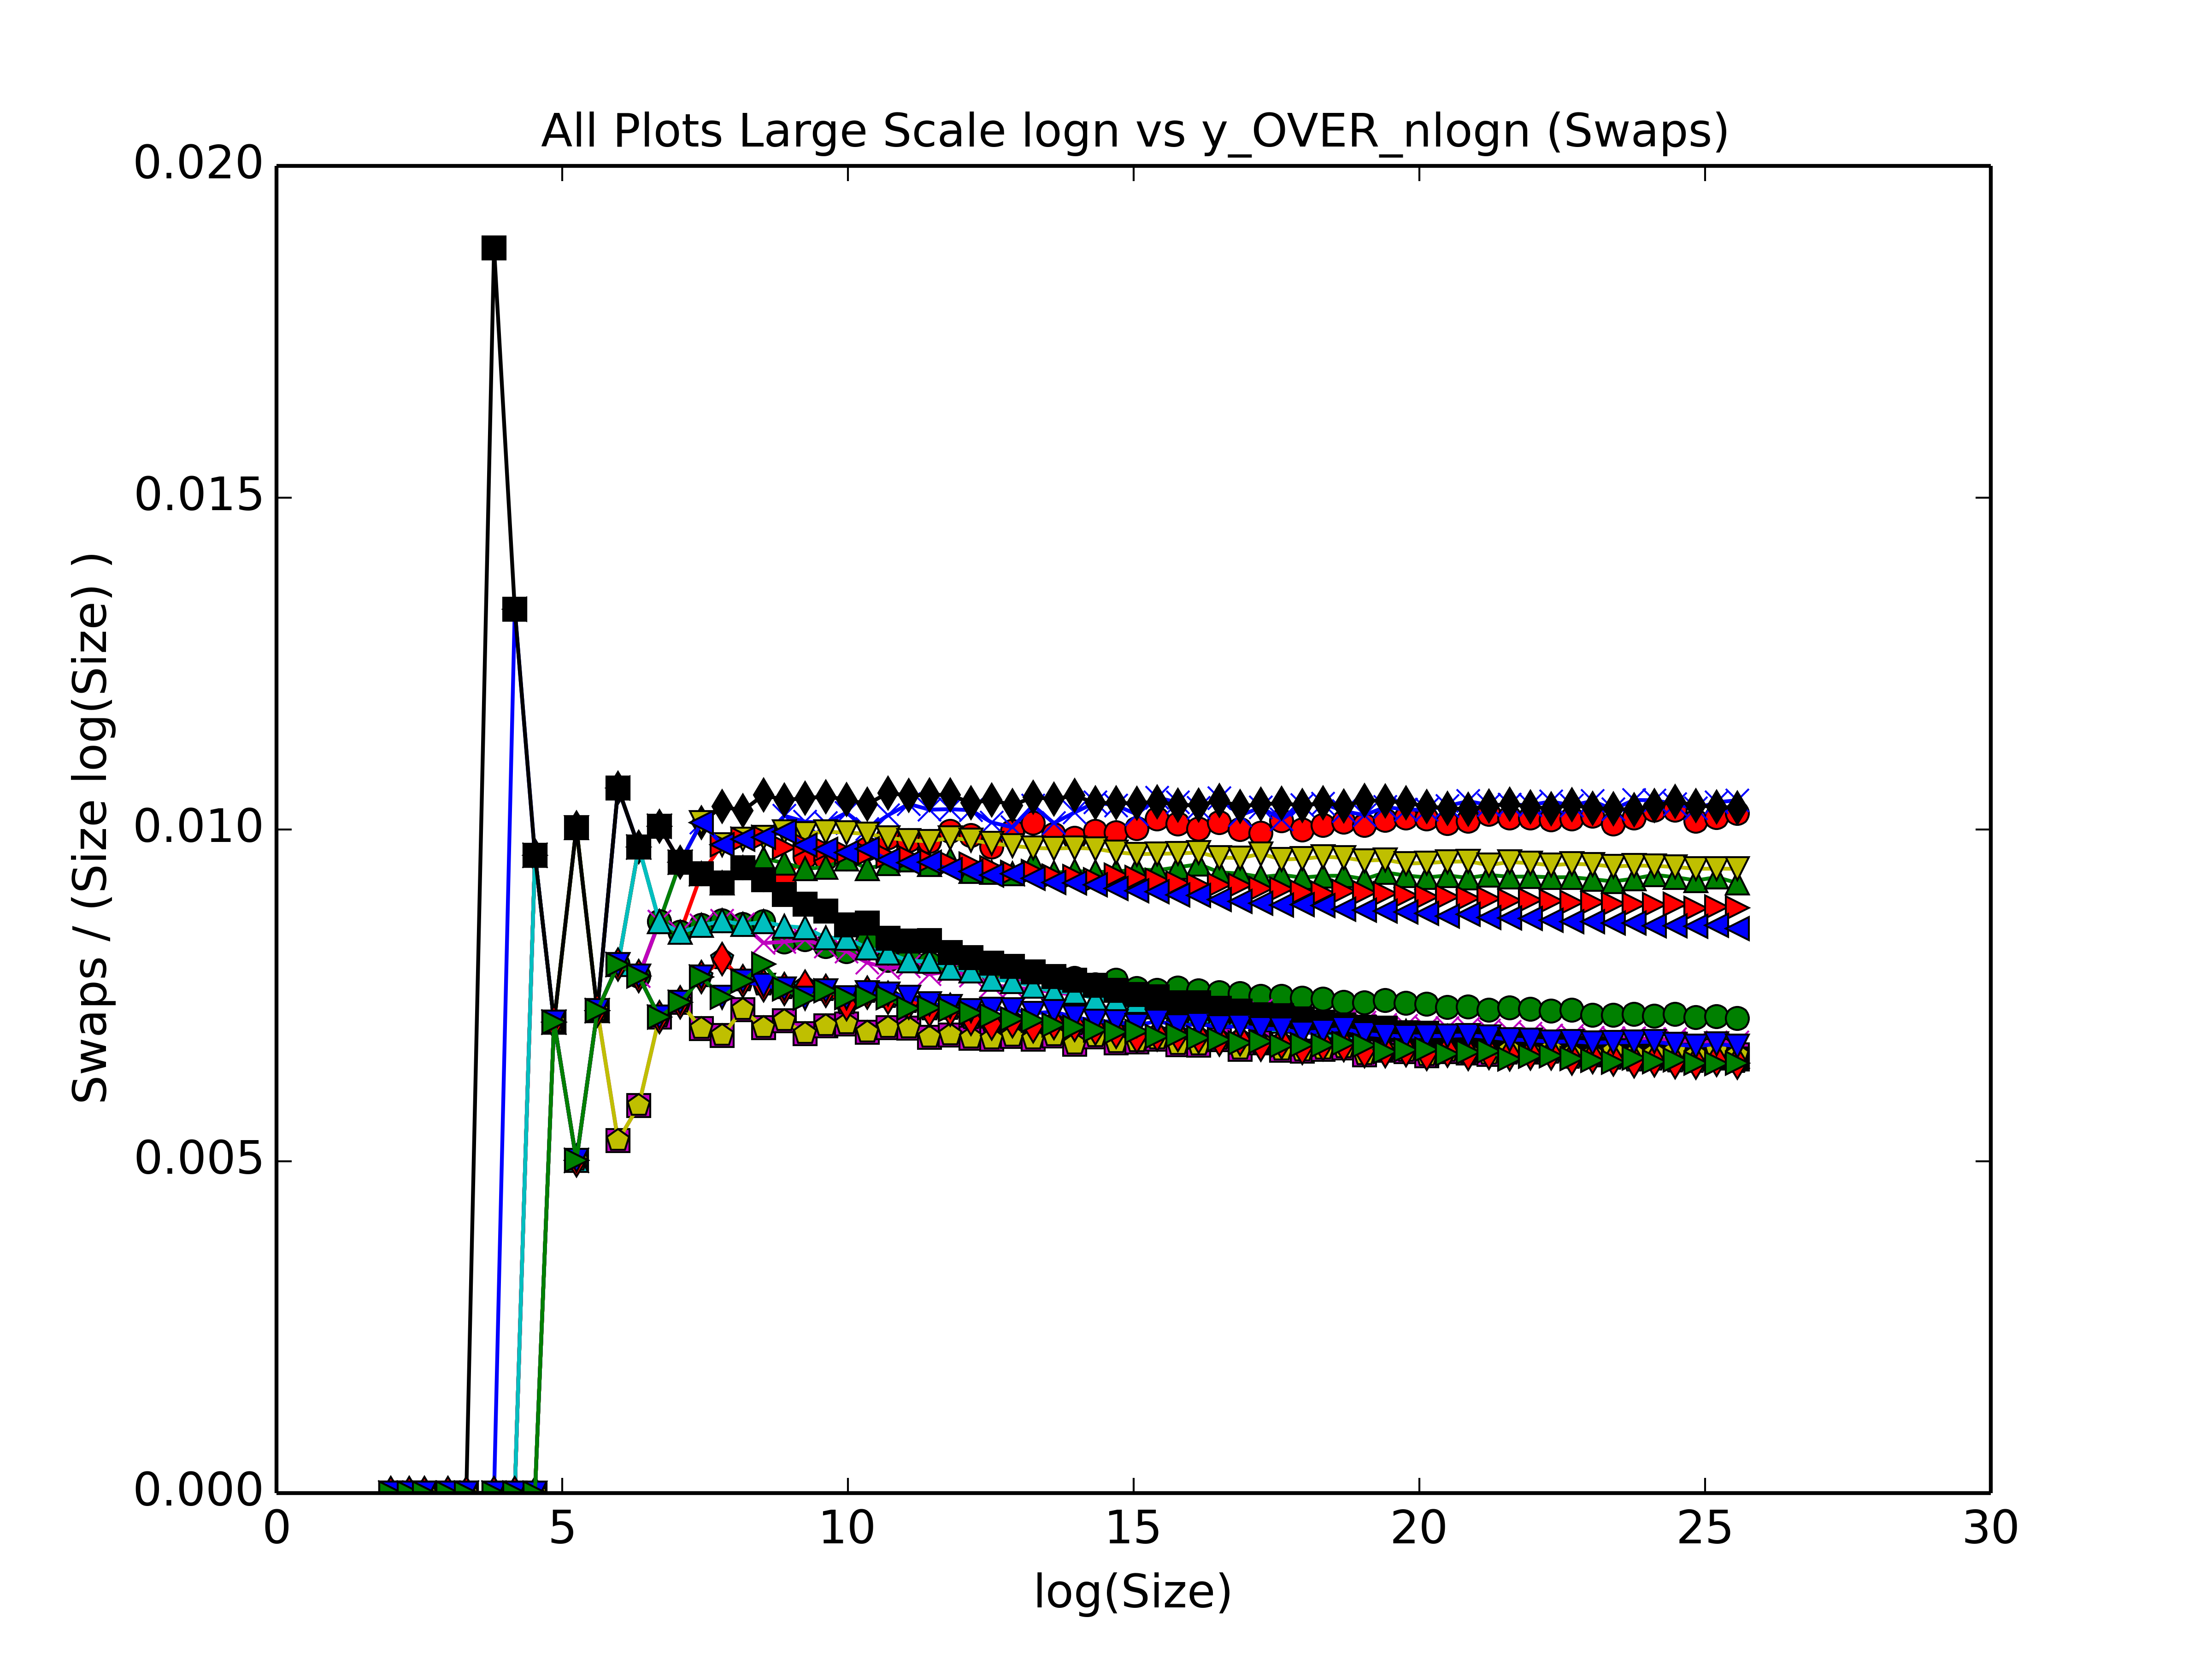
\includegraphics[width=120mm]{AllPlotsLargeScalelognvsy_OVER_nlogn_swap.png}
			\caption{A plot of the data from all the sorting algorithm}
			\label{fig:AllSortsLog}
		\end{center}
	\end{figure}

	Figure \ref{fig:PlotLegend} provides the legend for all of the plots. Note that for the plots we overlay the function:
	\begin{equation}
		A\cdot n\log(n) + B\cdot n + C \log(n)
		\label{eq:FitFunction}
	\end{equation}
	The nomenclature for the legend is as follows: 
	\begin{center}
		(Algorithm Name, Pivot Selection Method Index, Number of Pivots, is Insertion Sort used).
	\end{center}
	

\section{Analysis}
	\label{sec:Analysis}
	\subsection{Non-Linear Curve Fit}
		\label{subsec:CurveFit}

		With the data that has been collected we wish to be able to look at a whole data set and then quantitatively compare to other data sets. From our introduction of the different quicksort algorithms in section 	\label{sec:quicksortInto}, the asymptotic runtime of any of the described algorithms of the had one of the following forms:
		\begin{equation}
			A\cdot n\log(n) + B\cdot n + \BigOh{\log(n)}
		\end{equation}
		\begin{equation}
			A\cdot n\log(n) + \BigOh{n}
		\end{equation}
		\begin{equation}
			\BigOh{n\log(n)}
		\end{equation}
		In correspondence of this we will fit the data to the following equation:
		\begin{equation}
			A\cdot n\log(n) + B\cdot n + C\log(n)
			\label{eq:FitFunction}
		\end{equation}
		With the function parameters $A,B$ and $C$ were found using a non-linear curve fitting tool in the SciPy module in Python. Quantitatively, the fit function that was picked seems to result in good fits visually. Though the fit has less meaning do to the fact we don't have error bars on the data. A closer look at the reduced chi squared values of the fits leads us to believe that the fits are not good \cite{bevington1969data}. Thus we will treat the results from the best fit as qualitative.


	\subsection{Effect of Pivot Selection}
	\begin{figure}
		\centering
		\begin{minipage}{.5\textwidth}
		 	\centering
		 	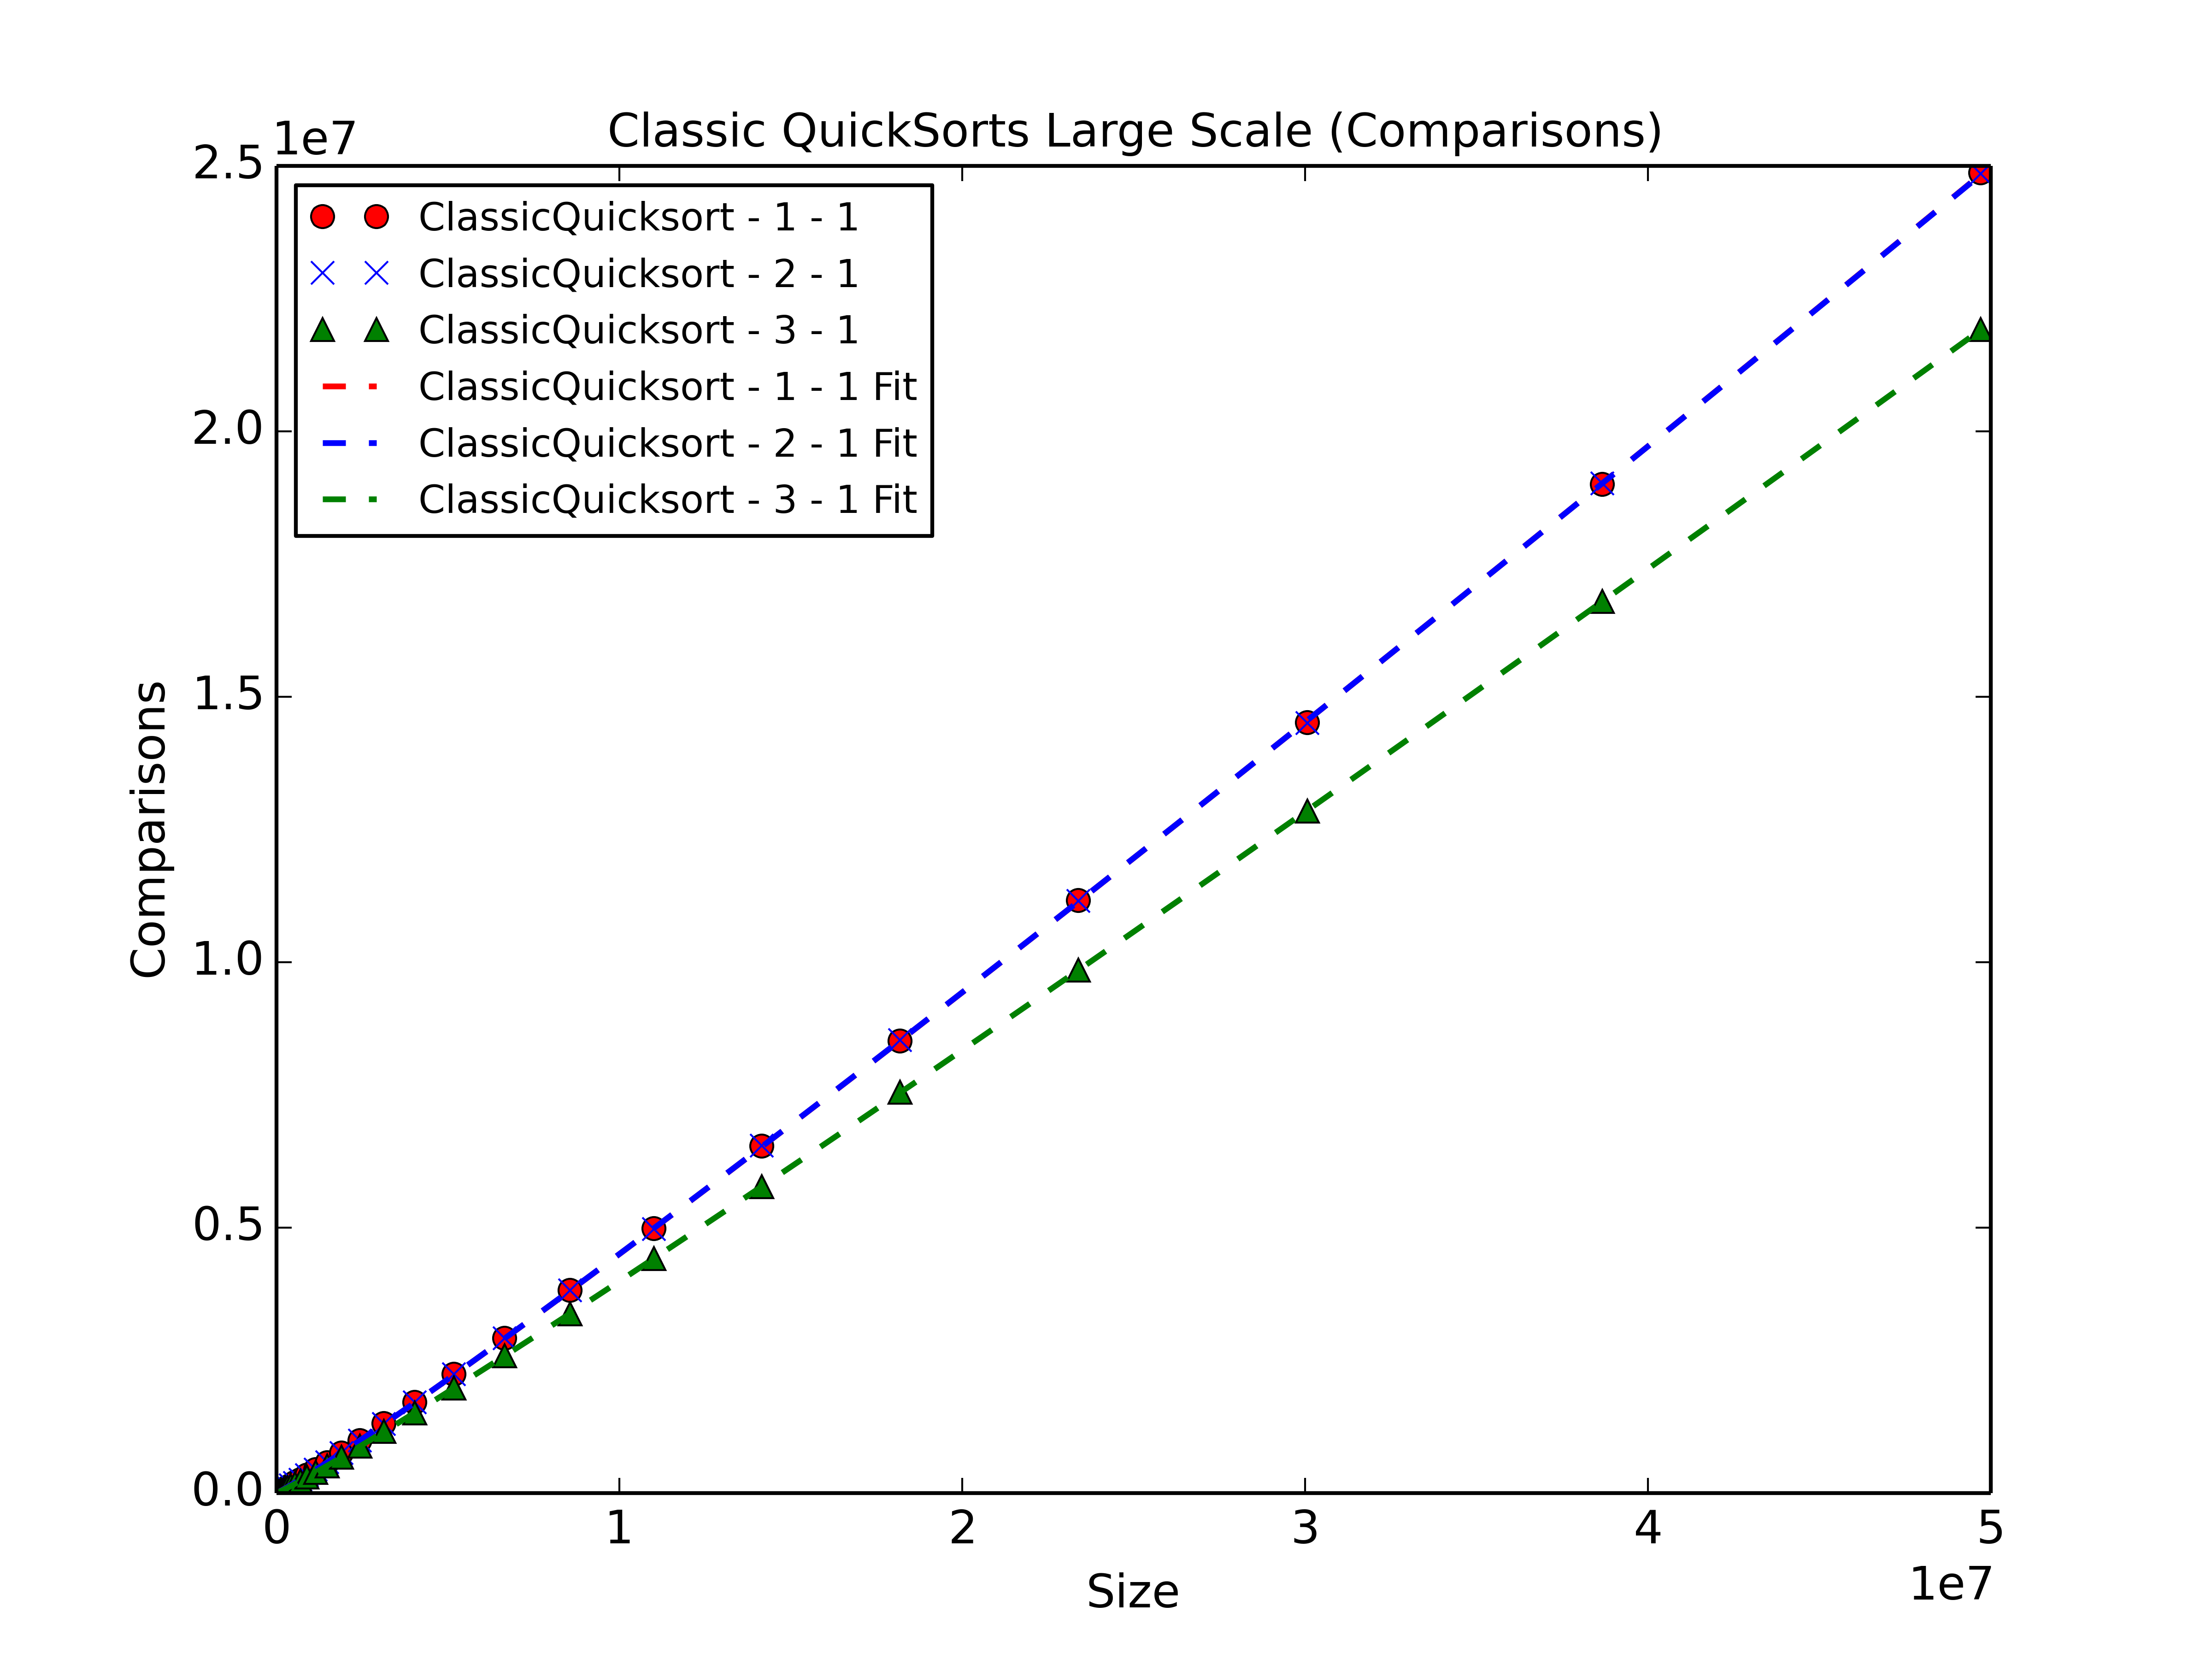
\includegraphics[width=\linewidth]{ClassicQuickSortsLargeScale_comp.png}
		\end{minipage}%
		\begin{minipage}{.5\textwidth}
		 	\centering
		 	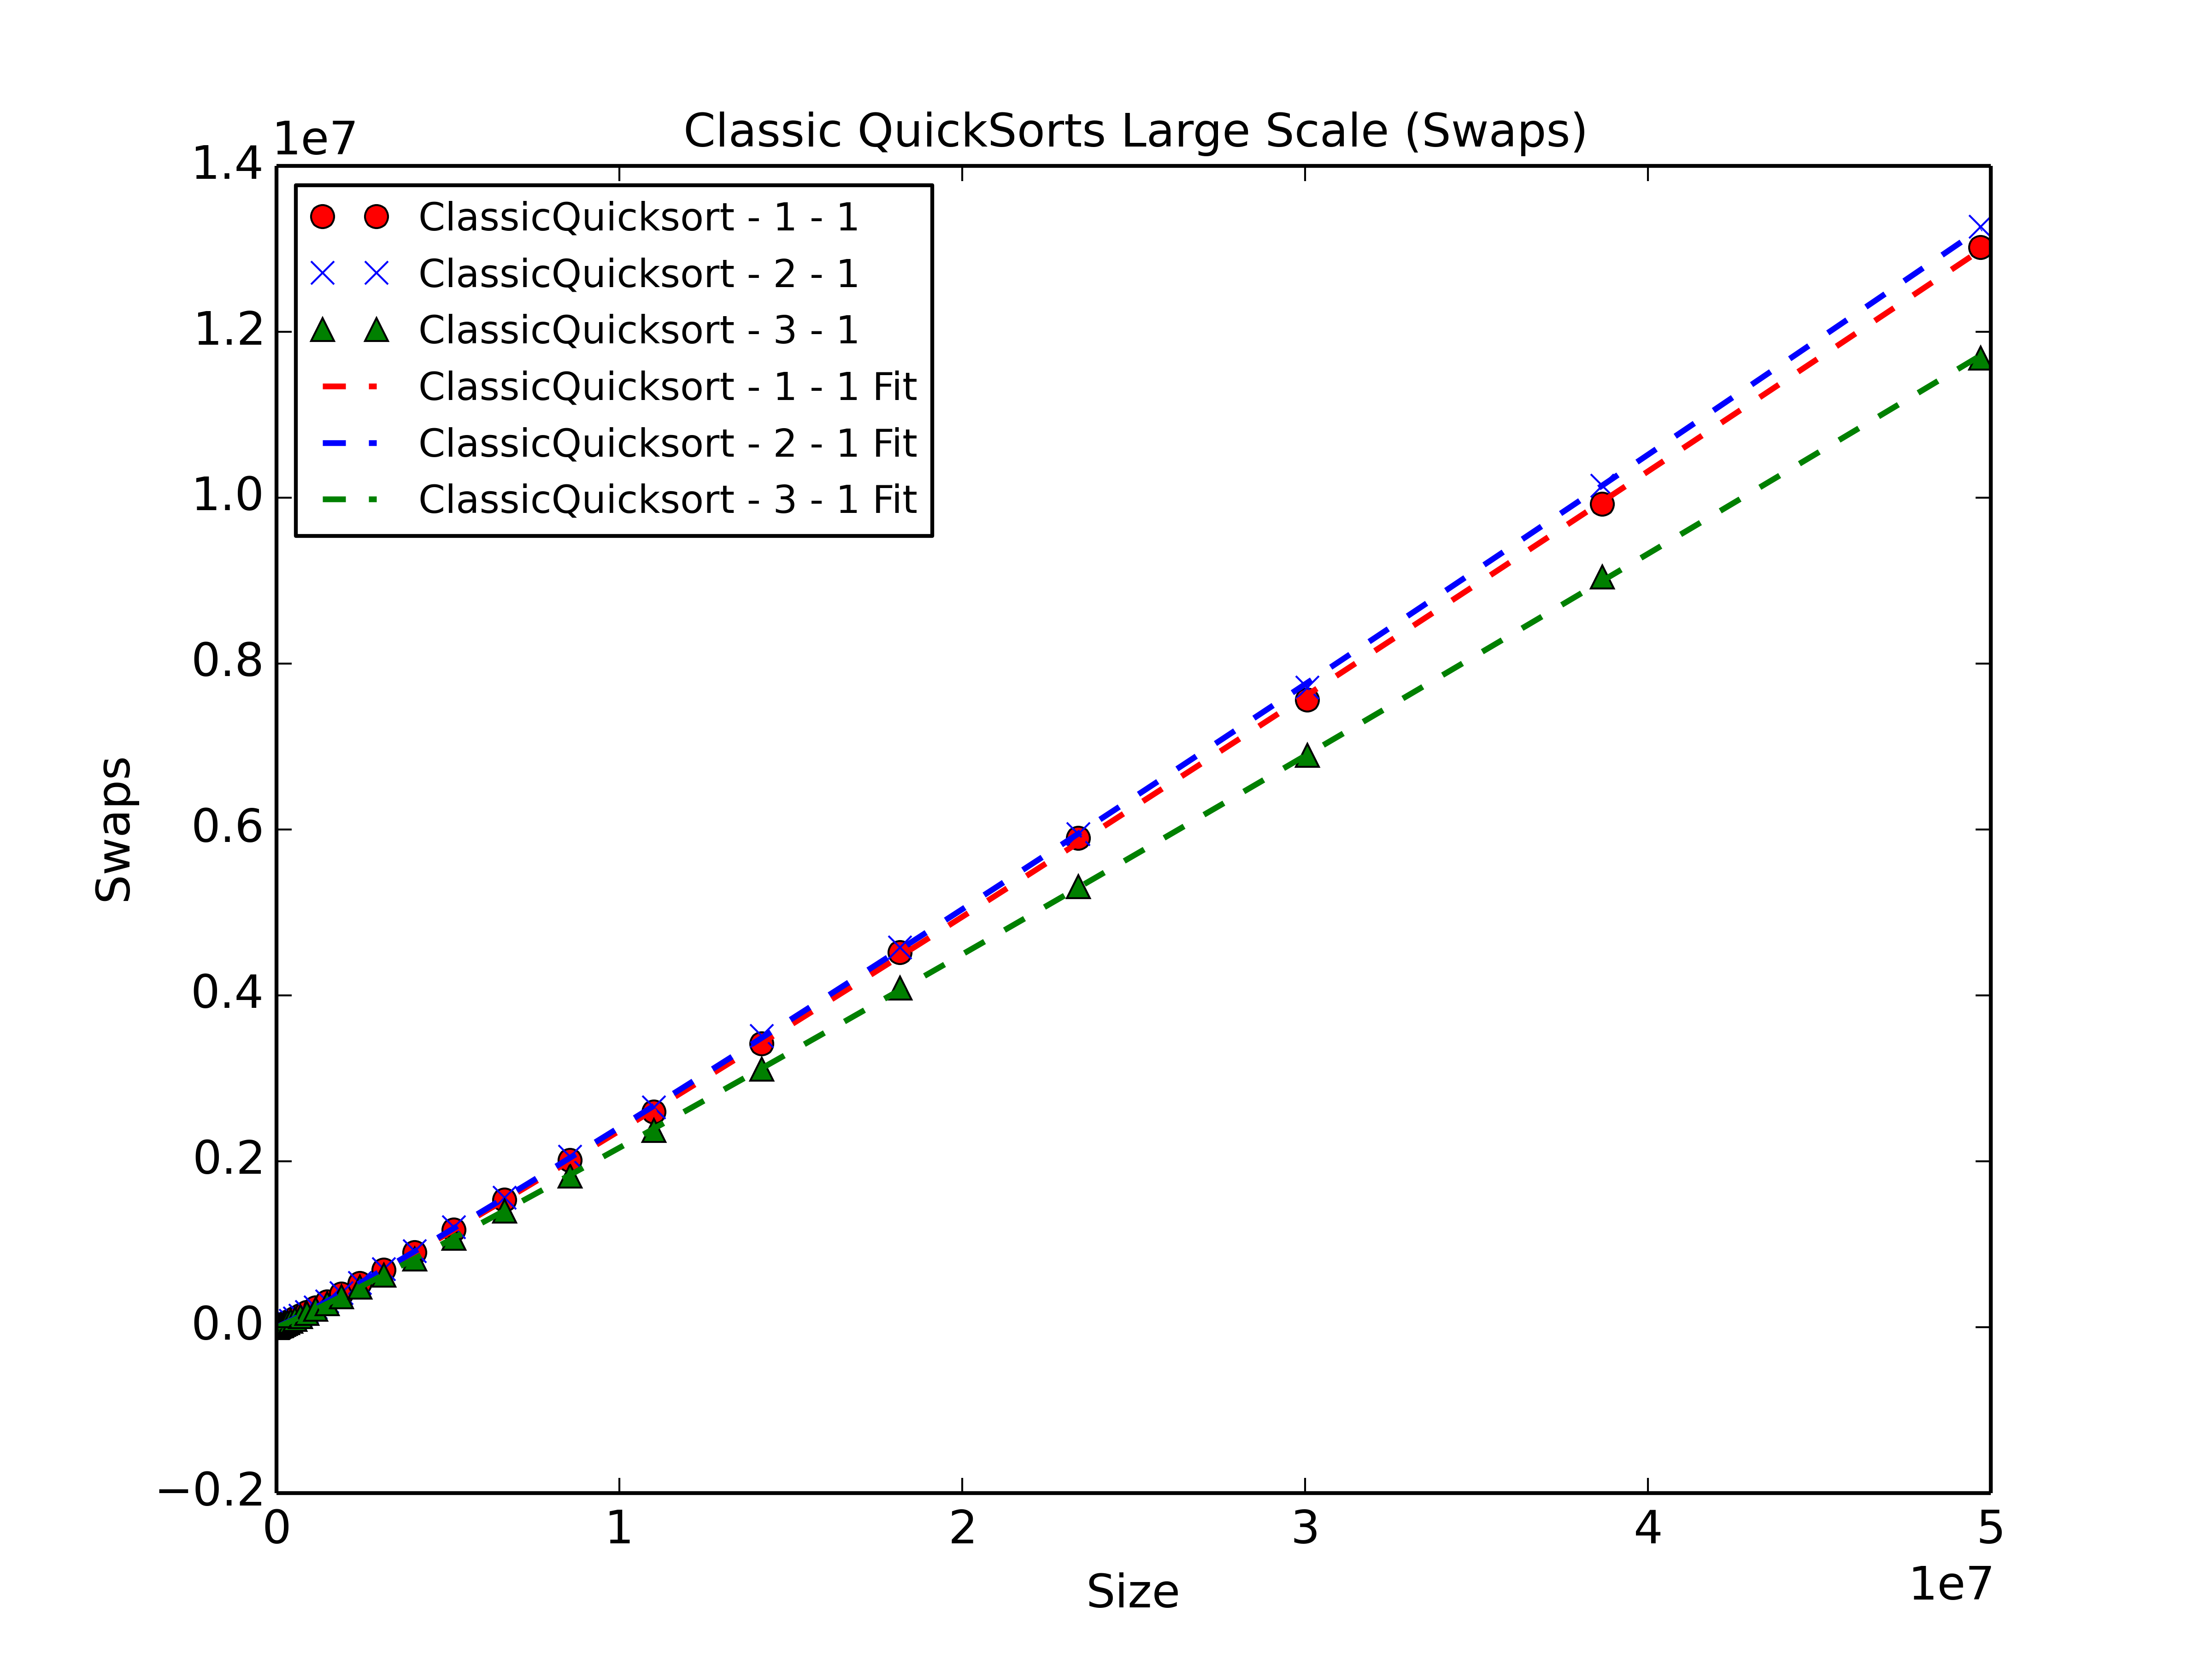
\includegraphics[width=\linewidth]{ClassicQuickSortsLargeScale_swap.png}
		\end{minipage}
		\caption{Swap and comparison counts for the classic quicksort.}
		\label{fig:classicSwapAndComp}
	\end{figure}

	In Figure \ref{fig:classicSwapAndComp} we can see that picking the pivot as the median of the fist, middle and last elements (green line) provides a significant decrease in comparisons and swaps compared to picking the first element (red line) or last element (blue line). We expect that picking any single element should provide no difference but we see that selecting the last element as the pivot is beneficial over picking the first element. We believe that this may be an artifact of the random number generator in Python's random module which documents that it should not be used for cryptographically secure applications suggesting the generator is in some way subpar. 

	%-----------------------------------------------------------------
	%Dual pivot graphs
	%-----------------------------------------------------------------
	\begin{figure}
		\centering
		\begin{minipage}{.5\textwidth}
		 	\centering
		 	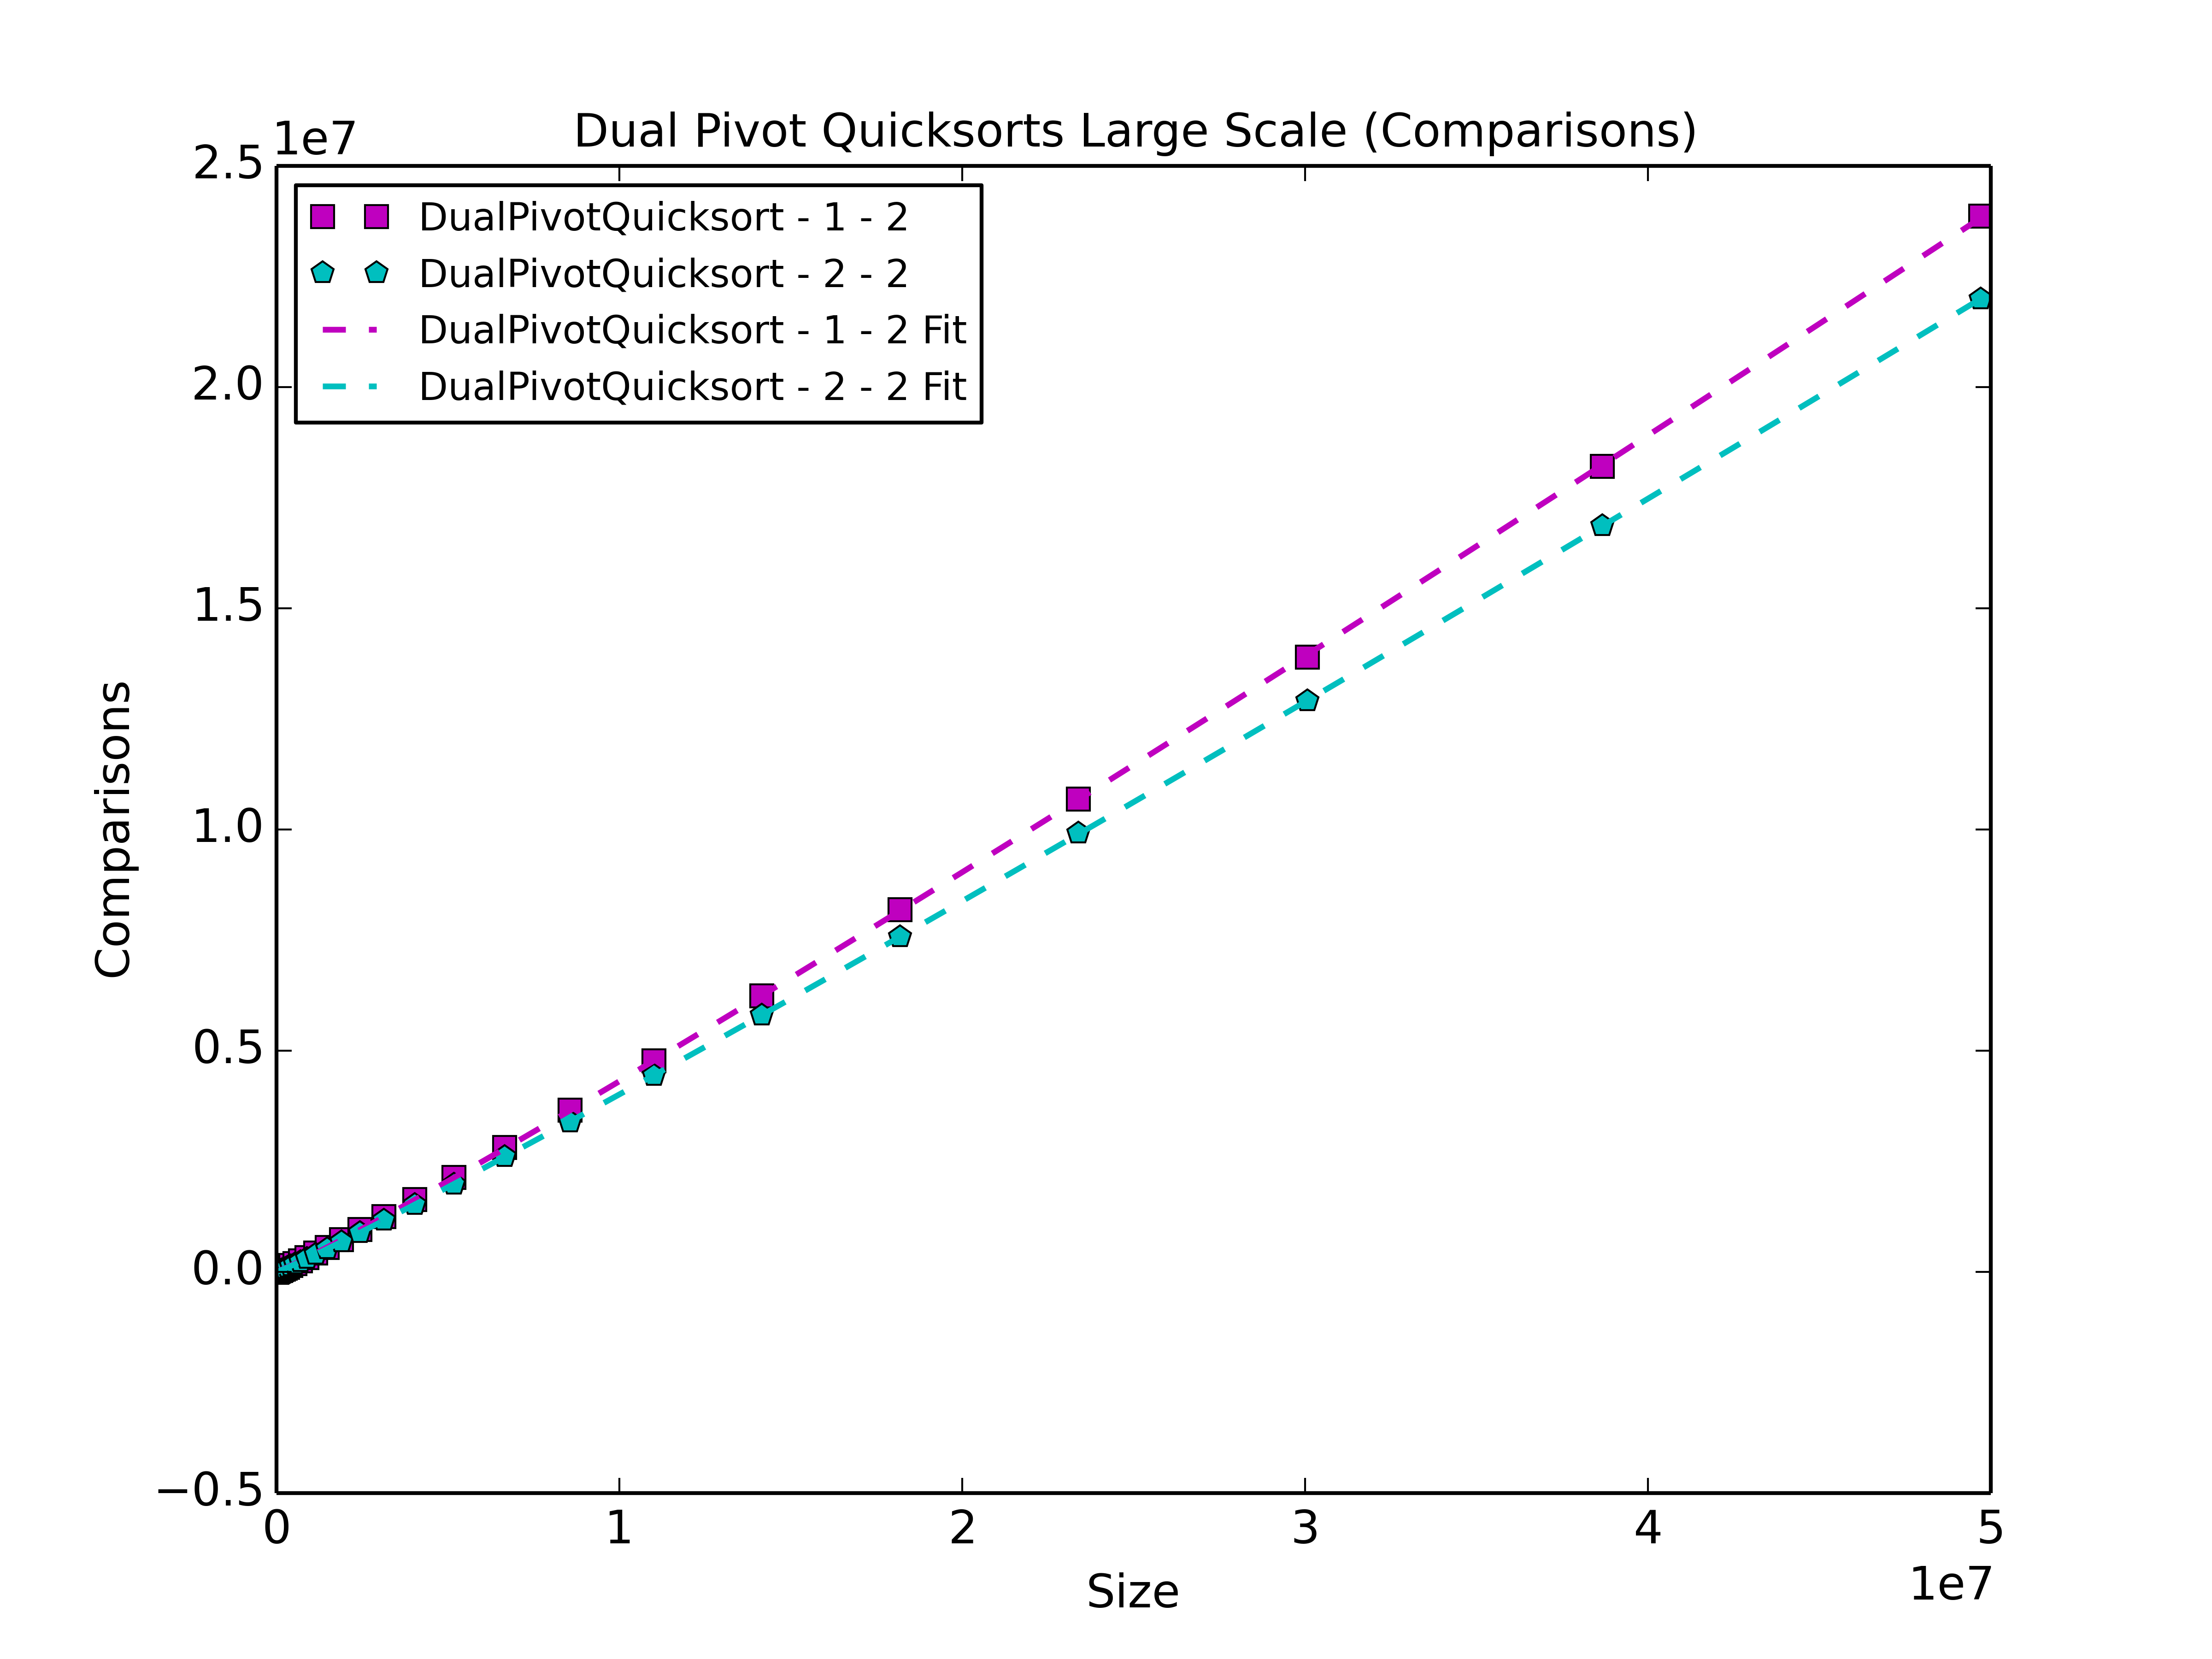
\includegraphics[width=.8\linewidth]{DualPivotQuicksortsLargeScale_comp}
		\end{minipage}%
		\begin{minipage}{.5\textwidth}
		 	\centering
		 	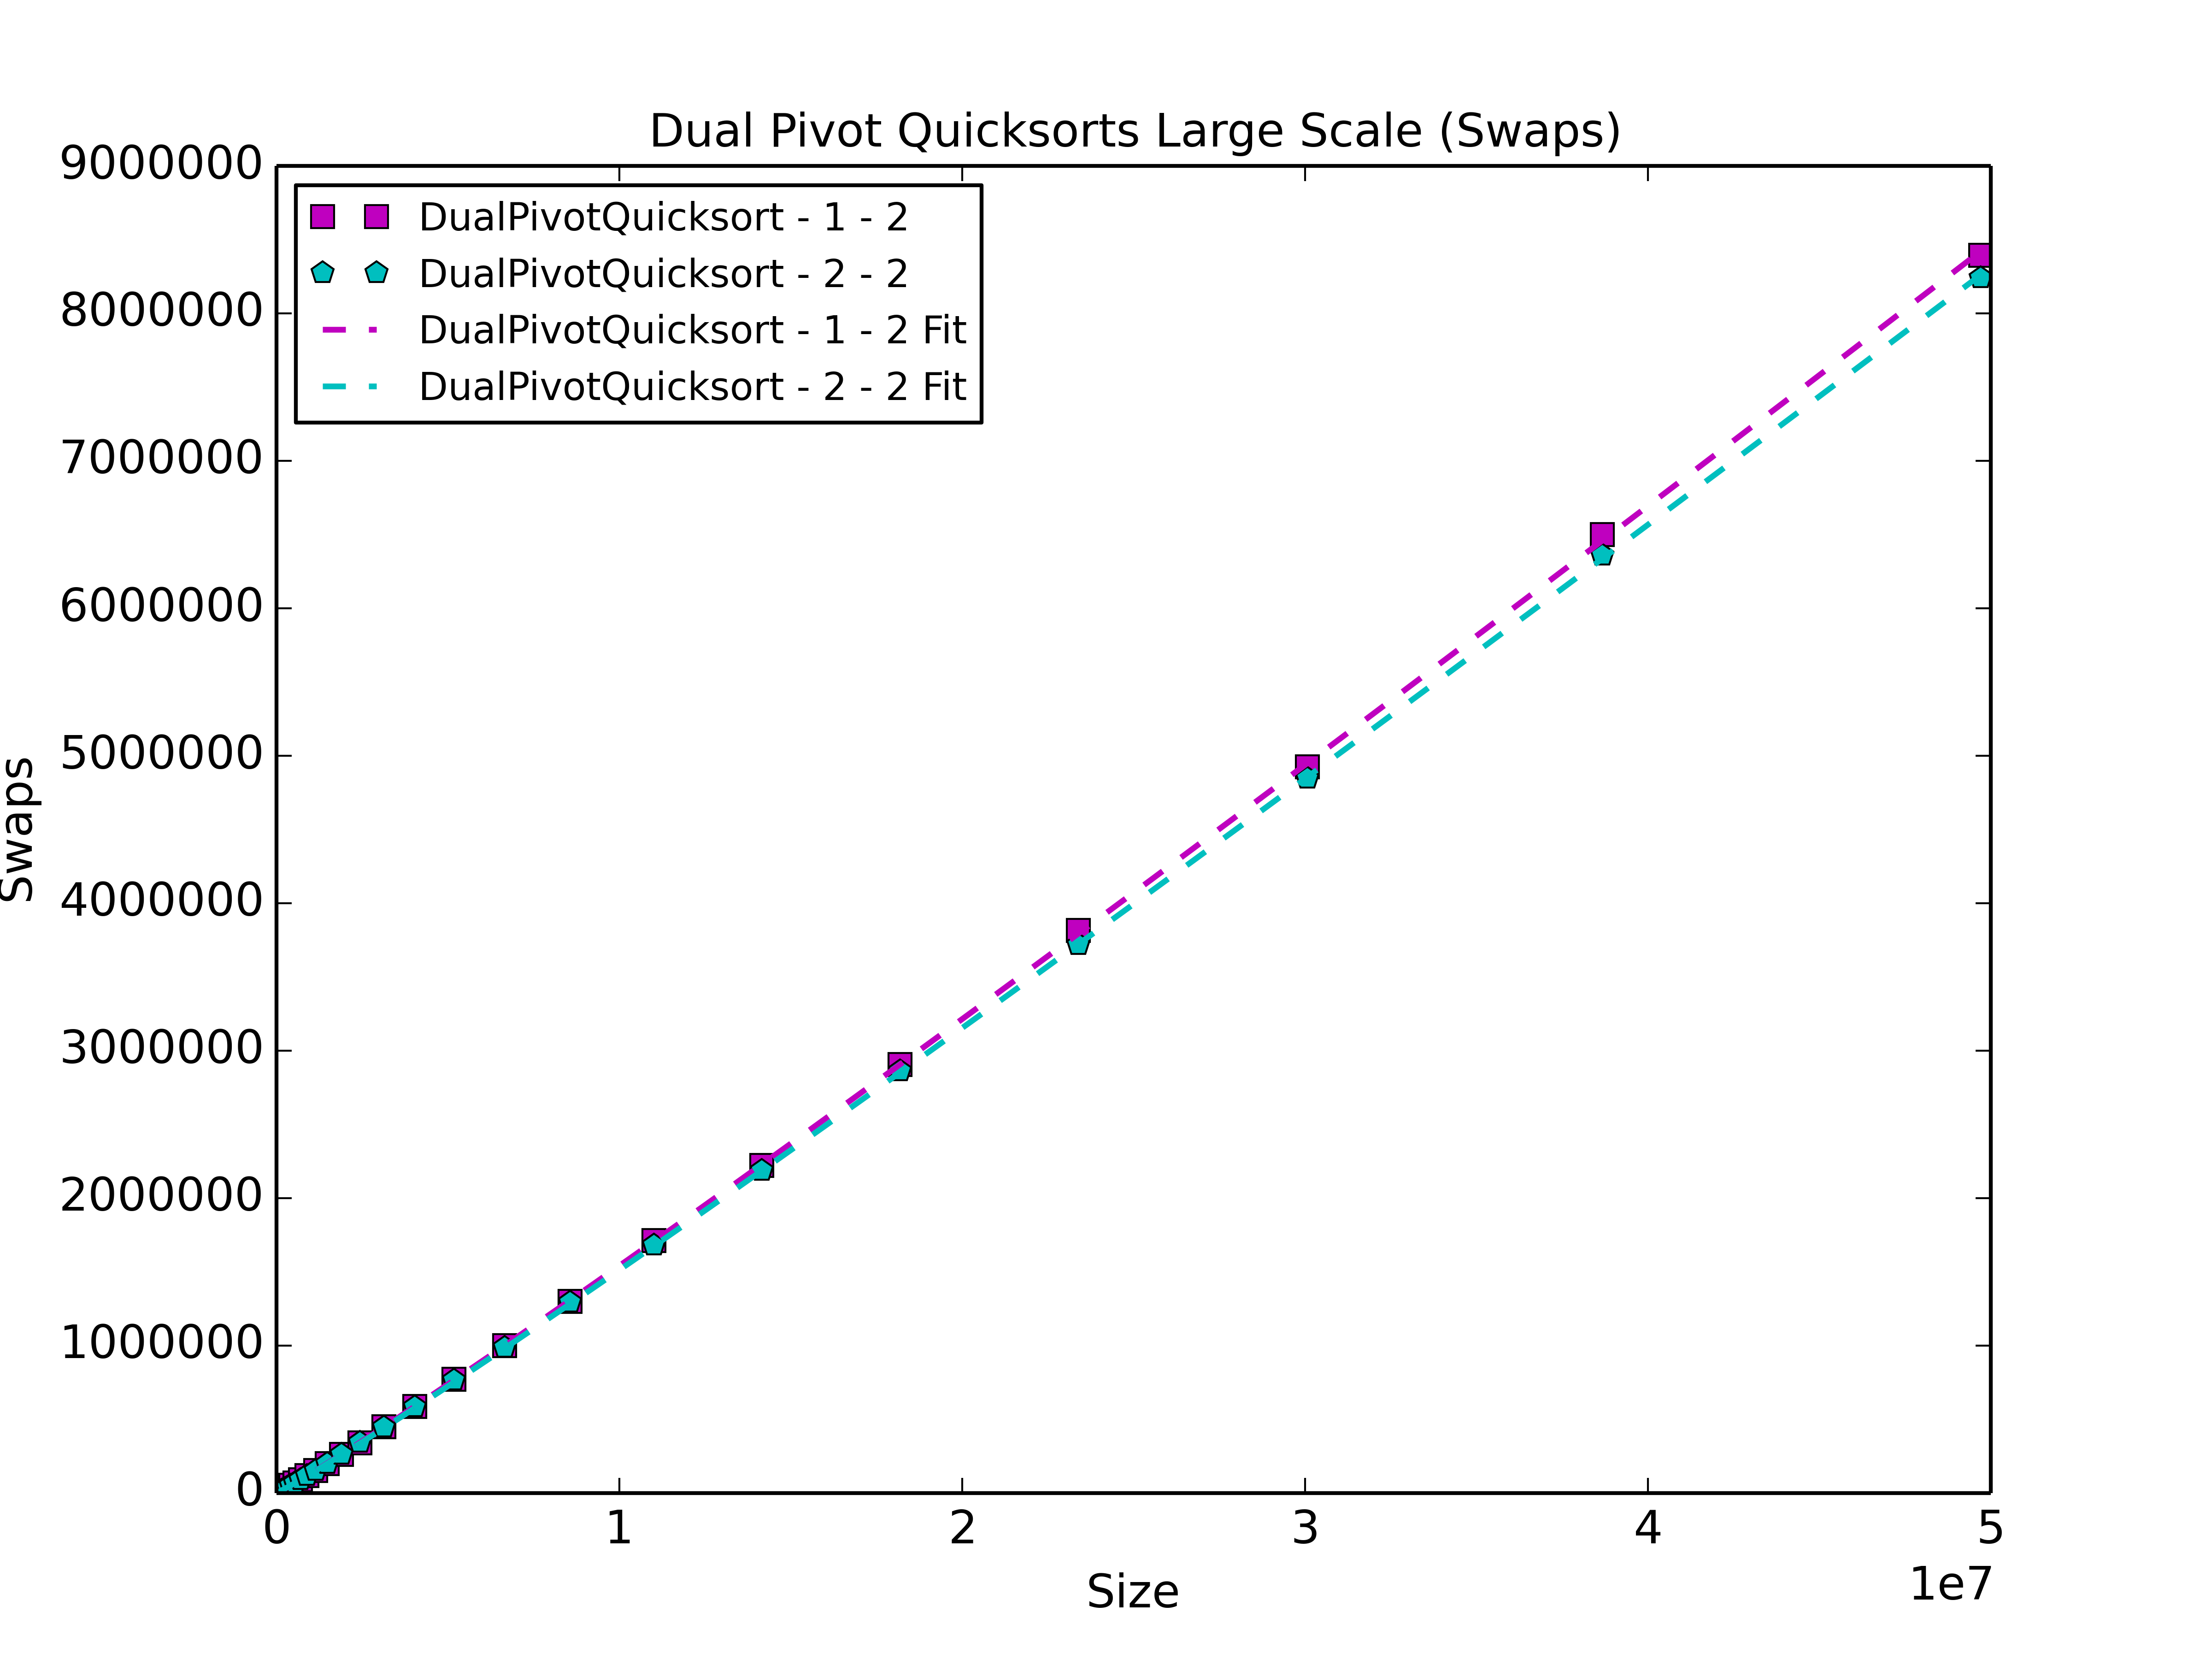
\includegraphics[width=.8\linewidth]{DualPivotQuicksortsLargeScale_swap}
		\end{minipage}
		\caption{Swap and comparison counts for the dual pivot quicksort.}
		\label{fig:dualSwapAndComp}
	\end{figure}

	%-----------------------------------------------------------------
	%Optimal Dual pivot graphs
	%-----------------------------------------------------------------
	\begin{figure}
		\centering
		\begin{minipage}{.5\textwidth}
		 	\centering
		 	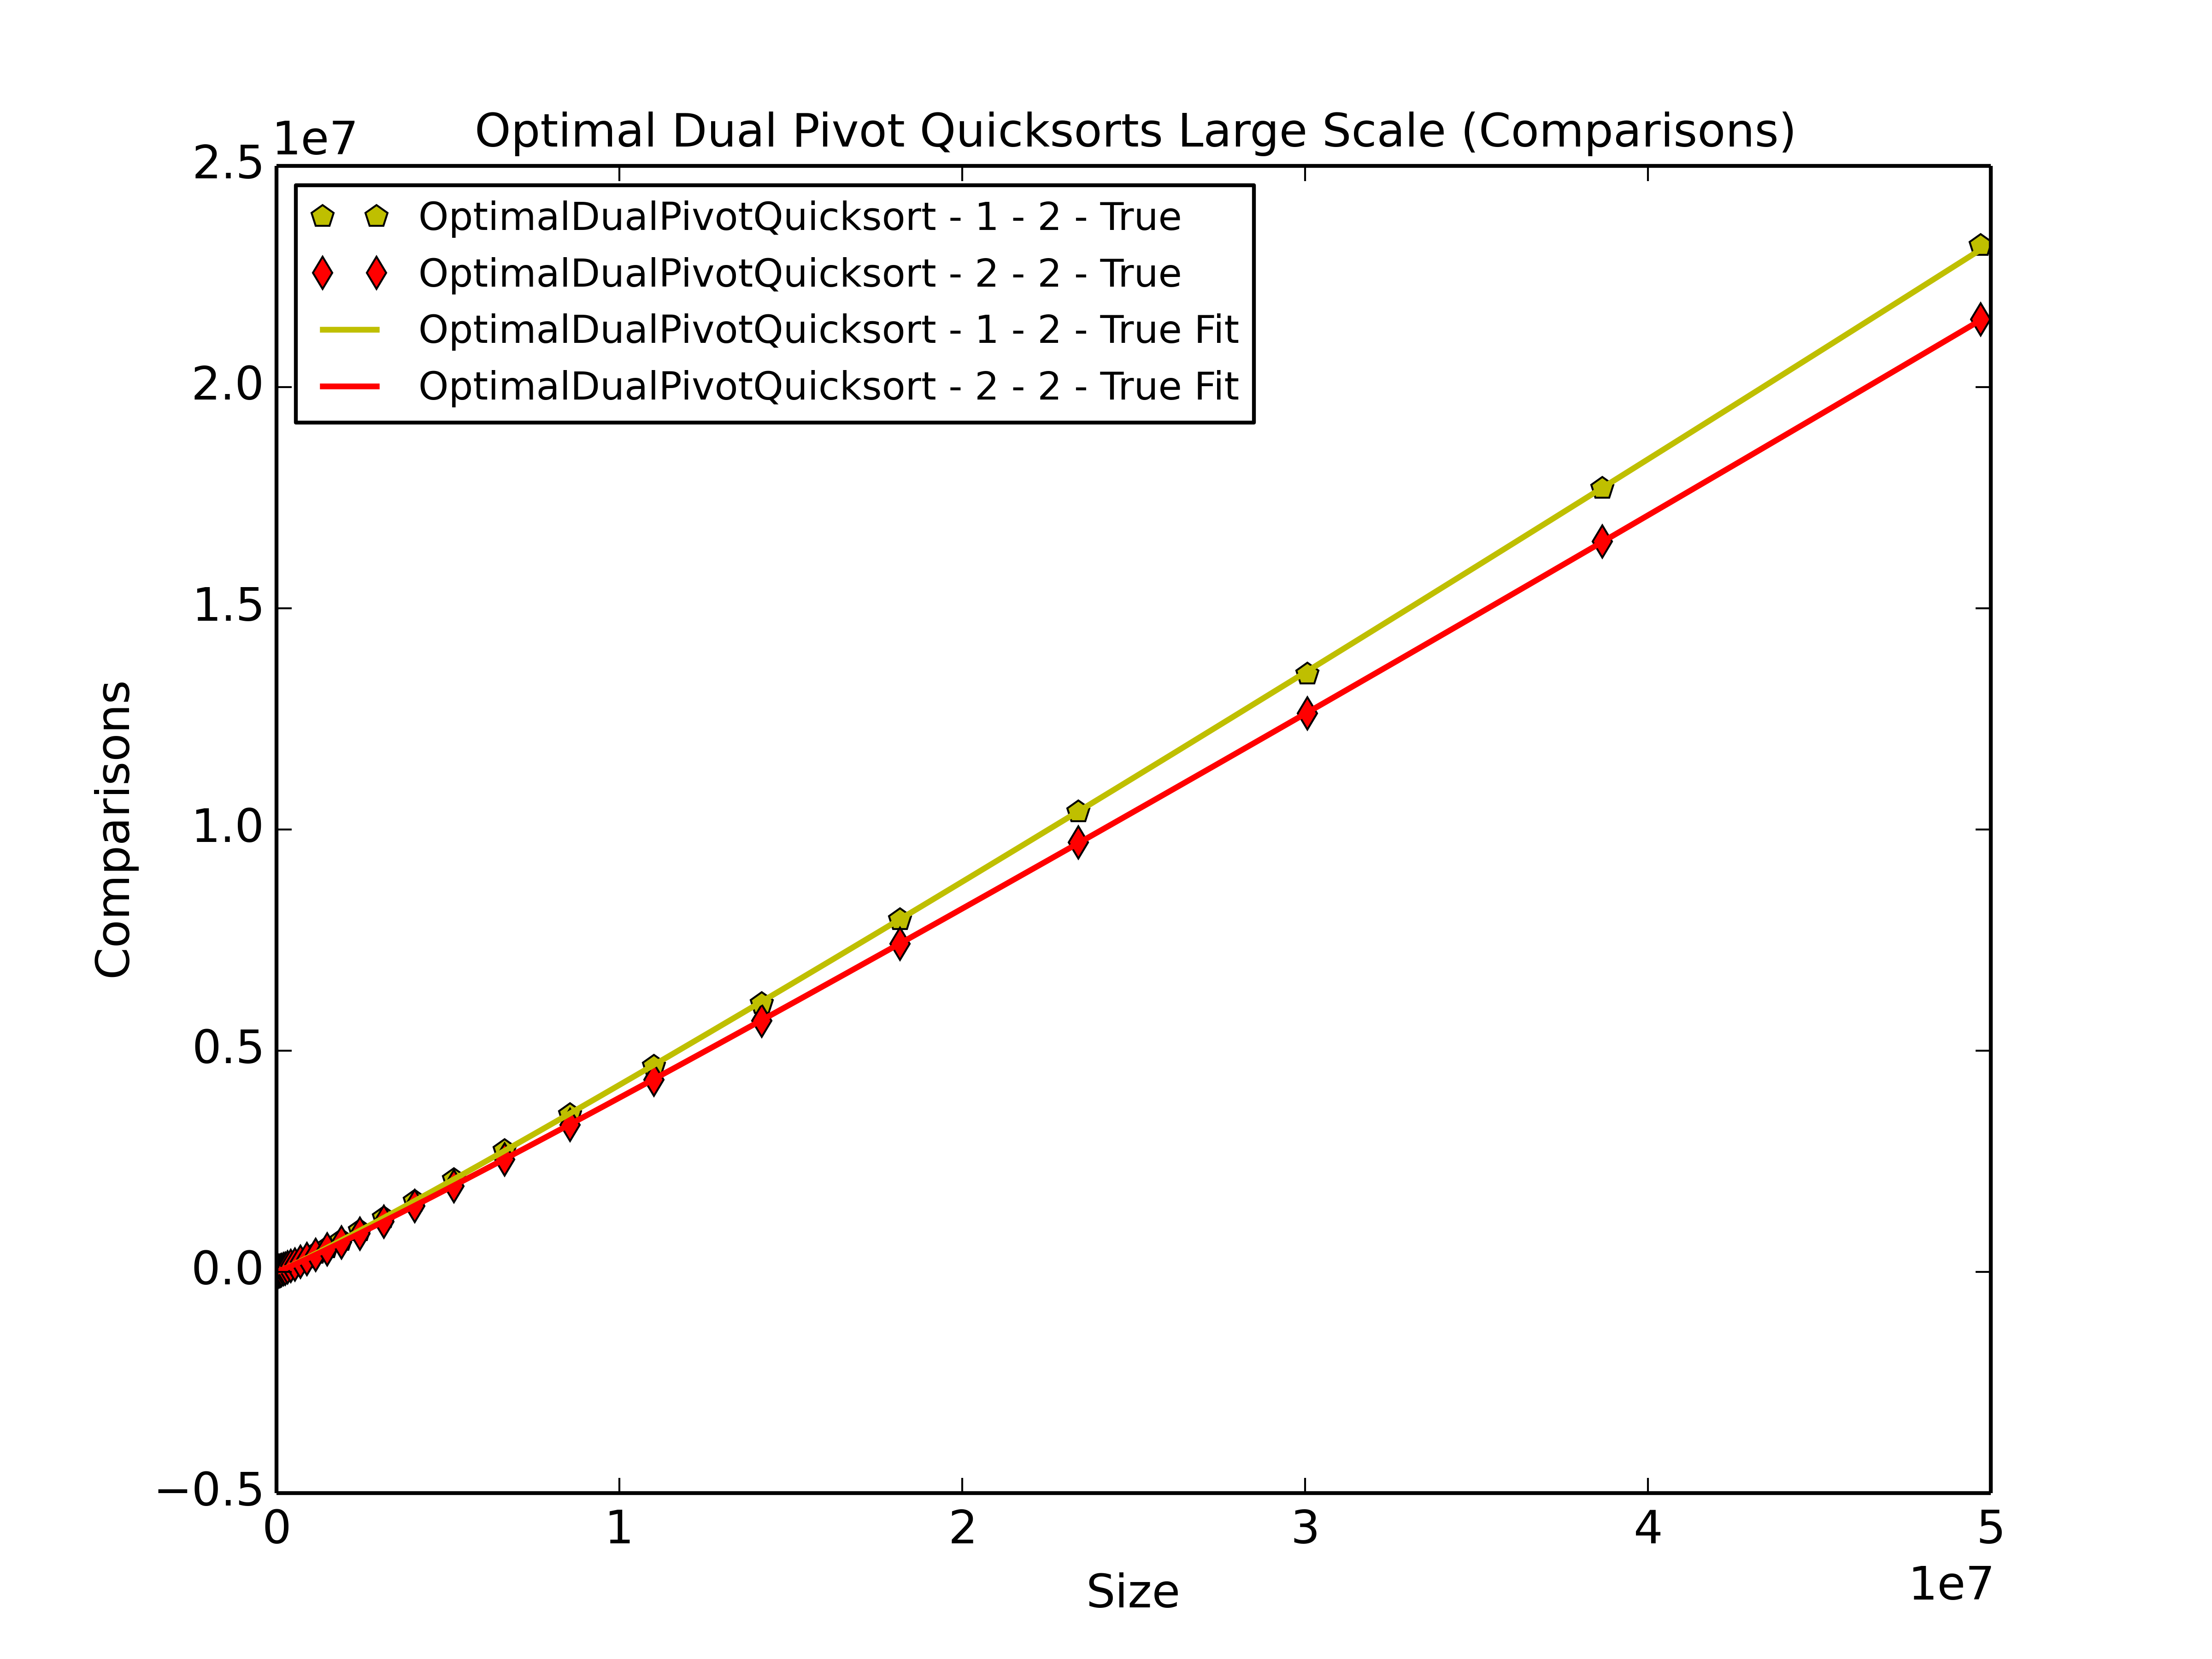
\includegraphics[width=.8\linewidth]{OptimalDualPivotQuicksortsLargeScale_comp.png}
		\end{minipage}%
		\begin{minipage}{.5\textwidth}
		 	\centering
		 	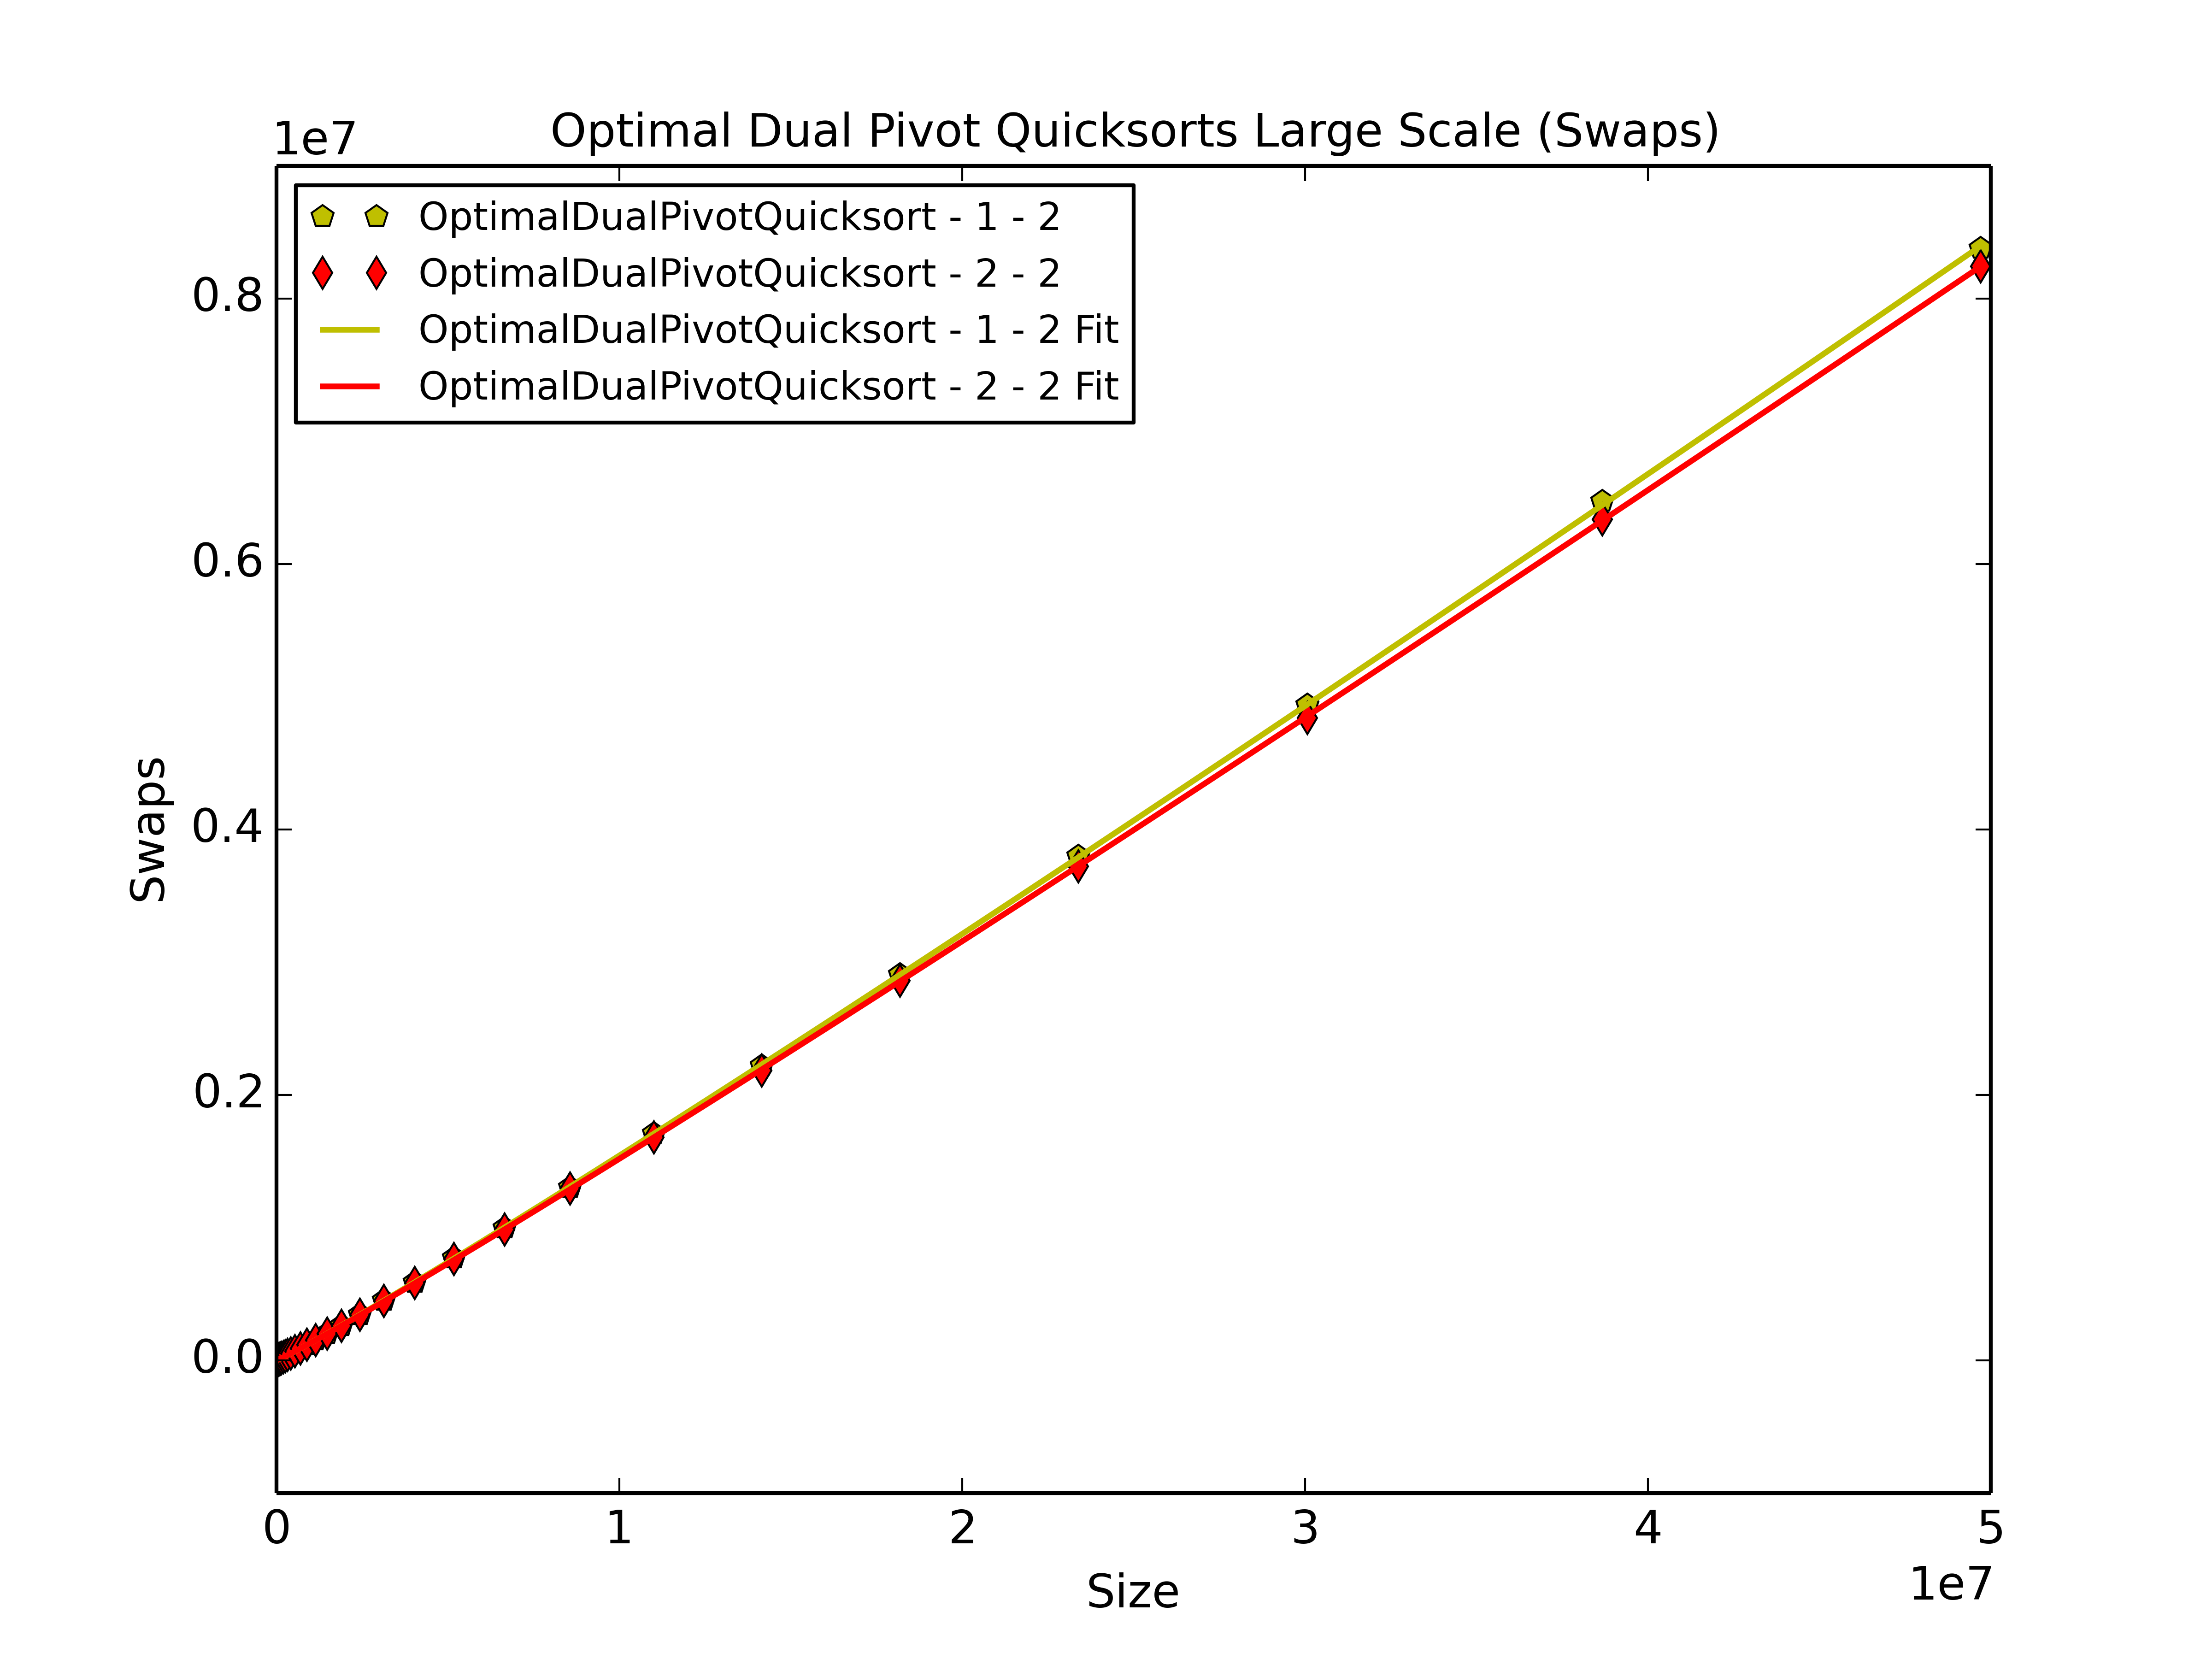
\includegraphics[width=.8\linewidth]{OptimalDualPivotQuicksortsLargeScale_swap.png}
		\end{minipage}
		\caption{Swap and comparison counts for the optimal dual pivot quicksort.}
		\label{fig:optimalDualSwapAndCount}
	\end{figure}

	Similar to the classic quicksort, we see in Figures \ref{fig:dualSwapAndComp} and \ref{fig:optimalDualSwapAndCount} that selecting pivots intelligently provides a benefit for the dual pivot quicksort and it's optimal counterpart. Interestingly, smart pivot selection has a large effect on the number of comparisons for both of the dual pivot quicksorts while having a less pronounced effect on the number of swaps. We believe that due to the larger number of pivots and the nature of the data we sorted there is a higher probability that each element will already be in it's correct partition and thus the effect of ``good'' pivots is less pronounced. Had the data been almost-sorted we believe that the effect of smart pivot selection would be more conspicuous.

		

\section{Discussion}
	\label{sec:Discussion}
	\subsection{$n\log(n)$ Trend}
		% Talk about \ref{fig:AllSortsLog}
		% This plot shows that the data is tapering off to a constant
		% But if you look at the axis, this is confirming the n log n
		% Behavior of the data and the algorithms
		
		A basic question to ask is if we are seeing the $n log(n)$ trend in all of the sort data we see. From Figure \ref{fig:AllSortsLog} we see plots of $\rfrac{y}{n \log(n)}$ (where $y$ is either the number of comparisons or swaps). As $n$ gets larger you can see that each curve is tending to a constant. Since the $\rfrac{y}{n \log(n)}$ approaches a constant, this indicates that $y$ is of $\BigOh{n}$. Which is consistent with the theory described in the introduction.
		%**********************************************************************
		% Reference the intro section for the part above.
		%**********************************************************************
		

	\subsection{Comparisons among Quicksorts}
		%Large Scale mass data
		%Comparisons :
		%   Optimized dual pivot quicksort is the best
		%   yaro, M-pivot sorts do well
		%   Heap Optimized m-pivot sorts do badly
		%Swaps :
		%   Heap Optimized Sorts still do badly relative to the rest.
		%   Classic quicksorts also doing badly.
		%   
		%   You can see two bands the bad ones as stated above
		%   and the not bad ones, which is everything else
		%
		%   When looking at the Three-Pivot-Quicksort it does surprisingly bad
		%   for the number of comparisons. Right up there with the classic and
		%   Heap-m-pivot sorts. Although it has a competitive number of swaps
		%   being operated.
		%   In fact when you look at the Three-Pivots-Plot you can see
		%   That the three-pivot-quicksort has the best number of swaps
		%   done of all the quicksorts that use three pivots.
	
		% Talk about the plots and how each sort algorithm does relative to the others.
		Preliminary observations on Figure \ref{fig:AllSorts} show that the optimal dual pivot quicksort had the lowest number of comparisons. This is as expected since it was designed to minimize the number of comparisons. Also the Yaroslavskiy and $M$-Pivot sort (for $M=3,4,5,6$) have a minimal number of comparisons. In contrast, the number of comparisons for all of the heap optimized $M$-pivot sorts are poor. Unexpectedly, the three pivot quicksort and classic quicksort both have performance comparable to that of the heap optimized $M$-pivot sorts. The thee pivot quicksort performs surprisingly few swap operations in comparison to the $M$-pivot quicksorts. 
		
		

		% Two pivot plots
		%Comparisons :
		%	We can start to see them split.
		%	Optimal Dual Pivot Quicksort [second option] still rocks.
		%	Dual Picot [1] and Optimal Dual Pivot [1] don't do well.
		%   It is small but you can see the trend lines starting to split at
		%   then end.
		%   you can see from the plot is that the second method
		%   of partition consistently produces a lower number of comparisons.
		%Swaps :
		%	They all do very similarly.
		%	Optimal Dual [1] and Dual Pivot [1] start to split away.[Do badly]
		%
		
		An observation from the two pivot quicksorts with pivot selection that selects the first and last element as the pivots don't do as well as the selection of the quartiles in the number of comparisons. This can be seen from figure \ref{fig:TwoPivot}. When looking at size vs. swaps in the two pivot there are no noteworthy differences. 
		
		% Three pivot plots
		%Comparisons :
		%	Interpretations Clear From plot.
		%	3-Pivot Sort is great then the Three-pivot-Quicksort
		%Swaps :
		%	Three-pivot-Quicksort is great then the 3-Pivot Sort
		%
		% In both cases heap 3-pivot sort is the worst.
		
		
		% All the M-pivot plots even with heap optimization
		%Comparisons :
		%	3,4,5-pivot sort are really good.
		%	All the heap-m-pivot sorts are not
		%Swaps :
		%	6-pivot sort is the best.
		%	Although 3,4,5-pivot sorts are good as well.
		%	All the heap-m-pivot sorts are not good.
		%
		% It seems odd that all the heap-optimized-m-pivot sorts do that badly.

		In comparisons between all the $M$-pivot sort algorithms, the ones without the heap optimization always did better. This is due to an implementation error. In the original description of the algorithm the heapfication of the array only happens on the very first call whereas in our implementation it occurs for every recursive call.

		%**********************************************************************
		% Qualitatively compare them with there fit coefficients
		%**********************************************************************

	\subsection{Fit Functions}
		% Talk about the fit values, remember we are treating these values as qualitative
		% Talk about best and worst algorithms in terms of swaps and comparisons
		% Remember that the fit coefficients table has been updated.
		% Talk about the other functions that we have tried to fit
		
		From tables \ref{tab:compFitCoeffA}, \ref{tab:compFitCoeffB}, \ref{tab:compFitCoeffC}, \ref{tab:swapFitCoeffA}, \ref{tab:swapFitCoeffB} and \ref{tab:swapFitCoeffC} the fit coefficients for the data collected is summarized based of equation \ref{eq:FitFunction}. For the sake of asymptotic comparison between the algorithms we only focus on the fit parameter $A$. Based on these coefficients the optimal dual pivot quicksort with quartile pivot selection is shown to be the best quick sort algorithm based in regards to the number of comparisons. Conversely, the heap-optimized $M$ pivot quicksort for $M=6$, is the worst algorithm based in regards to the number of comparisons. The classic quicksort algorithms using the median-of-three for pivot selection has incredibly poor swap performance. The best algorithm for reducing the number of swaps is the basic $M$-pivot sort algorithm with $M=6$. But the only algorithm with competitive runtimes for both metrics is Yaroslavskiy's dual pivot quicksort algorithm.
		

	\subsection{Future Work}
		\label{subsec:FutureStuff}
		% Talk about looking for more sorts
		% Talk about other distributions for random numbers
		% Talk about applying on nearly sorted arrays.
		% Talk about trying to measure time
		% Test M=1 and M=2 for the M-Pivot quick sort
		% Test with insertion sort off
		% More data values on the same entires.
		While our tests only examined the performance of these quicksorts on lists of nearly unique numbers, we believe that examining their comparison and swap counts on different ``kinds'' of lists provides just as much, if not more, insight. This is especially true for concerns of their worst-case performance. Lists of numbers which can be modelled by a Gaussian or Poisson distribution may provide some insight into the behaviour of these quicksorts on real world data. Additionally, sorting lists in pseudo-sorted or sorted order will provide data for the worst-case performance of these sorts. Another potentially interesting may be one where elements of the list are chosen uniformly at random but where the range of the selected elements is less than the length of the list, thus guaranteeing value repetition. 

		Comparing these sorts against other sorts may also be of use. Other popular ``efficient'' sorts such as the merge sort or timsort can provide good points of reference for the performance of the quicksort. This can be especially useful if more ``kinds'' of lists are used as mentioned previously. We also believe that comparing the M-Pivot quicksort with $M=1$ and $M=2$ with the other one and two pivot sorts can result in potentially interesting graphs and analysis. We also believe that implementing the optimizations presented by Edmonson \cite{edmondson2005m} on the quicksorts other than the M-Pivot Quicksort can prove useful in determining their true effectiveness.


		

\section{Conclusion}
	\label{sec:Conclusionn}
	We have implemented several variations of the quicksort and explored their efficiencies in regards to total number of swaps and comparisons. Our results show that Yaroslavskiy's quicksort is the highest overall performer while the heap optimized $M$-pivot quicksorts performed the worse. Our results also validate the idea that intelligent pivot selection provides a measurable and significant effect on the overall performance of quicksorts. We find that for lists of nearly unique numbers, selecting a median of three and first and third quartiles of five provide good performance to developer time ratios. Our results also show that the optimal dual pivot quicksort performs better than Yaroslavskiy's quicksort in regards to total number of comparisons as claimed by \cite{Aumuller:2013:OPD:2525857.2525862} while the two sorts are nearly identical in swap count.

	Overall, the $M$-Pivot quicksorts performed well. The $M$-Pivot quicksort with $M=3$ performed better than the three pivot quicksort of Kushagra et al. \cite{kushagra2013multi}. We also find that at small scales, the choice of quicksort makes little difference. 
	Yaro better than we thought. M pivot surprisingly good. Partitioning is subtlely difficult. Yaroslavs partition alg is amazing \cite{Aumuller:2013:OPD:2525857.2525862} \cite{Wild:2012:ACA:2404160.2404231}. 
	



%**********************************************************************
% Place the following in the appendix
%**********************************************************************

\section{Fit Coefficients}
	\label{sec:FitCoefficients}

	% (name,medianSelection,numPivots,usedInsertionSort)
	%***************************************************************************************************
	% FIT PARAMETERS FOR COMPARISONS
	%***************************************************************************************************
	\begin{table}
		\begin{center}
			\begin{tabular}{|r|c|c|c}
				\hline
								Sort Method              &   $A_{\text{comparisons}}$      \\ \hline \hline
				                Classic Quicksort - 1 - 1 &   $0.02151 \pm  0.00019$ \\ \hline
				                Classic Quicksort - 2 - 1 &   $0.02135 \pm  0.00017$ \\ \hline
				                Classic Quicksort - 3 - 1 &   $0.01807 \pm  0.00006$ \\ \hline
				              DualPivot Quicksort - 1 - 2 &   $0.02014 \pm  0.00018$ \\ \hline
				              DualPivot Quicksort - 2 - 2 &   $0.01772 \pm  0.00007$ \\ \hline
				 Heap Optimized M-Pivot Quicksort - 1 - 3 &   $0.02778 \pm  0.00014$ \\ \hline
				 Heap Optimized M-Pivot Quicksort - 1 - 4 &   $0.02788 \pm  0.00015$ \\ \hline
				 Heap Optimized M-Pivot Quicksort - 1 - 5 &   $0.02842 \pm  0.00025$ \\ \hline
				 Heap Optimized M-Pivot Quicksort - 1 - 6 &   $0.02869 \pm  0.00011$ \\ \hline
				                M-Pivot Quicksort - 1 - 3 &   $0.01970 \pm  0.00009$ \\ \hline
				                M-Pivot Quicksort - 1 - 4 &   $0.02076 \pm  0.00015$ \\ \hline
				                M-Pivot Quicksort - 1 - 5 &   $0.02165 \pm  0.00010$ \\ \hline
				                M-Pivot Quicksort - 1 - 6 &   $0.02386 \pm  0.00014$ \\ \hline
				     Optimal Dual Pivot Quicksort - 1 - 2 &   $0.01959 \pm  0.00019$ \\ \hline
				     Optimal Dual Pivot Quicksort - 2 - 2 &   $0.01744 \pm  0.00007$ \\ \hline
				            Three Pivot Quicksort - 1 - 3 &   $0.02587 \pm  0.00009$ \\ \hline
				           Yaroslavskiy Quicksort - 1 - 2 &   $0.01796 \pm  0.00010$ \\ \hline
			\end{tabular}
			\caption{Summary table coefficients of the non-linear fit for the parameter $A$ on the comparison data.}
			\label{tab:compFitCoeffA}
		\end{center}
	\end{table}


	\begin{table}
		\begin{center}
			\begin{tabular}{|r|c|c|c}
				\hline
								Sort Method              &   $B_{\text{comparisons}}$      \\ \hline \hline
				                Classic Quicksort - 1 - 1 &   $-0.05025 \pm  0.00469$ \\ \hline
				                Classic Quicksort - 2 - 1 &   $-0.04634 \pm  0.00428$ \\ \hline
				                Classic Quicksort - 3 - 1 &   $-0.02126 \pm  0.00163$ \\ \hline
				              DualPivot Quicksort - 1 - 2 &   $-0.03650 \pm  0.00465$ \\ \hline
				              DualPivot Quicksort - 2 - 2 &   $-0.01045 \pm  0.00183$ \\ \hline
				 Heap Optimized M-Pivot Quicksort - 1 - 3 &   $-0.05055 \pm  0.00355$ \\ \hline
				 Heap Optimized M-Pivot Quicksort - 1 - 4 &   $-0.05152 \pm  0.00368$ \\ \hline
				 Heap Optimized M-Pivot Quicksort - 1 - 5 &   $-0.04639 \pm  0.00626$ \\ \hline
				 Heap Optimized M-Pivot Quicksort - 1 - 6 &   $-0.03889 \pm  0.00280$ \\ \hline
				                M-Pivot Quicksort - 1 - 3 &   $-0.01917 \pm  0.00220$ \\ \hline
				                M-Pivot Quicksort - 1 - 4 &   $-0.01716 \pm  0.00391$ \\ \hline
				                M-Pivot Quicksort - 1 - 5 &   $-0.00902 \pm  0.00244$ \\ \hline
				                M-Pivot Quicksort - 1 - 6 &   $-0.03206 \pm  0.00366$ \\ \hline
				     Optimal Dual Pivot Quicksort - 1 - 2 &   $-0.03580 \pm  0.00490$ \\ \hline
				     Optimal Dual Pivot Quicksort - 2 - 2 &   $-0.01266 \pm  0.00165$ \\ \hline
				            Three Pivot Quicksort - 1 - 3 &   $-0.04282 \pm  0.00232$ \\ \hline
				           Yaroslavskiy Quicksort - 1 - 2 &   $-0.01636 \pm  0.00251$ \\ \hline
			\end{tabular}
			\caption{Summary table coefficients of the non-linear fit for the parameter $B$ on the comparison data.}
			\label{tab:compFitCoeffB}
		\end{center}
	\end{table}

	\begin{table}
		\begin{center}
			\begin{tabular}{|r|c|c|c}
				\hline
								Sort Method              &   $C_{\text{comparisons}}$      \\ \hline \hline
				                Classic Quicksort - 1 - 1 &  $ 121.34341 \pm  99.97322$ \\ \hline
				                Classic Quicksort - 2 - 1 &  $  78.33233 \pm  91.31275$ \\ \hline
				                Classic Quicksort - 3 - 1 &  $  22.52742 \pm  34.75034$ \\ \hline
				              DualPivot Quicksort - 1 - 2 &  $  52.22569 \pm  99.17037$ \\ \hline
				              DualPivot Quicksort - 2 - 2 &  $ -53.25104 \pm  39.07336$ \\ \hline
				 Heap Optimized M-Pivot Quicksort - 1 - 3 &  $  94.09226 \pm  75.71998$ \\ \hline
				 Heap Optimized M-Pivot Quicksort - 1 - 4 &  $ 124.92512 \pm  78.46872$ \\ \hline
				 Heap Optimized M-Pivot Quicksort - 1 - 5 &  $  56.97527 \pm 133.52044$ \\ \hline
				 Heap Optimized M-Pivot Quicksort - 1 - 6 &  $  29.84293 \pm  59.67899$ \\ \hline
				                M-Pivot Quicksort - 1 - 3 &  $  51.60730 \pm  46.87649$ \\ \hline
				                M-Pivot Quicksort - 1 - 4 &  $  49.35746 \pm  83.31083$ \\ \hline
				                M-Pivot Quicksort - 1 - 5 &  $   4.76647 \pm  52.03322$ \\ \hline
				                M-Pivot Quicksort - 1 - 6 &  $ 136.38815 \pm  77.96382$ \\ \hline
				     Optimal Dual Pivot Quicksort - 1 - 2 &  $  56.95127 \pm 104.39452$ \\ \hline
				     Optimal Dual Pivot Quicksort - 2 - 2 &  $ -26.20004 \pm  35.22097$ \\ \hline
				            Three Pivot Quicksort - 1 - 3 &  $ -17.79746 \pm  49.38183$ \\ \hline
				           Yaroslavskiy Quicksort - 1 - 2 &  $   0.73204 \pm  53.59187$ \\ \hline
			\end{tabular}
			\caption{Summary table coefficients of the non-linear fit for the parameter $C$ on the comparison data.}
			\label{tab:compFitCoeffC}
		\end{center}
	\end{table}



	%***************************************************************************************************
	% FIT PARAMETERS FOR SWAPS
	%***************************************************************************************************



	\begin{table}
		\begin{center}
			\begin{tabular}{|r|c|c|c}
				\hline
								Sort Method              &   $A_{\text{swap}}$      \\ \hline \hline
				                Classic Quicksort - 1 - 1 &   $0.01026 \pm  0.00017$ \\ \hline
				                Classic Quicksort - 2 - 1 &   $0.01095 \pm  0.00016$ \\ \hline
				                Classic Quicksort - 3 - 1 &   $0.00848 \pm  0.00012$ \\ \hline
				              DualPivot Quicksort - 1 - 2 &   $0.00629 \pm  0.00010$ \\ \hline
				              DualPivot Quicksort - 2 - 2 &   $0.00606 \pm  0.00006$ \\ \hline
				 Heap Optimized M-Pivot Quicksort - 1 - 3 &   $0.01004 \pm  0.00009$ \\ \hline
				 Heap Optimized M-Pivot Quicksort - 1 - 4 &   $0.00898 \pm  0.00004$ \\ \hline
				 Heap Optimized M-Pivot Quicksort - 1 - 5 &   $0.00809 \pm  0.00004$ \\ \hline
				 Heap Optimized M-Pivot Quicksort - 1 - 6 &   $0.00759 \pm  0.00005$ \\ \hline
				                M-Pivot Quicksort - 1 - 3 &   $0.00672 \pm  0.00006$ \\ \hline
				                M-Pivot Quicksort - 1 - 4 &   $0.00605 \pm  0.00003$ \\ \hline
				                M-Pivot Quicksort - 1 - 5 &   $0.00535 \pm  0.00003$ \\ \hline
				                M-Pivot Quicksort - 1 - 6 &   $0.00513 \pm  0.00003$ \\ \hline
				     Optimal Dual Pivot Quicksort - 1 - 2 &   $0.00629 \pm  0.00010$ \\ \hline
				     Optimal Dual Pivot Quicksort - 2 - 2 &   $0.00606 \pm  0.00006$ \\ \hline
				            Three Pivot Quicksort - 1 - 3 &   $0.00635 \pm  0.00006$ \\ \hline
				           Yaroslavskiy Quicksort - 1 - 2 &   $0.00586 \pm  0.00005$ \\ \hline
			\end{tabular}
			\caption{Summary table coefficients of the non-linear fit for the parameter $A$ on the swap data.}
			\label{tab:swapFitCoeffA}
		\end{center}
	\end{table}


	\begin{table}
		\begin{center}
			\begin{tabular}{|r|c|c|c}
				\hline
								Sort Method              &   $B_{\text{swap}}$      \\ \hline \hline
				                Classic Quicksort - 1 - 1 &   $ -0.00132 \pm  0.00442$ \\ \hline
				                Classic Quicksort - 2 - 1 &   $ -0.01411 \pm  0.00417$ \\ \hline
				                Classic Quicksort - 3 - 1 &   $  0.01903 \pm  0.00298$ \\ \hline
				              DualPivot Quicksort - 1 - 2 &   $  0.00824 \pm  0.00264$ \\ \hline
				              DualPivot Quicksort - 2 - 2 &   $  0.01080 \pm  0.00153$ \\ \hline
				 Heap Optimized M-Pivot Quicksort - 1 - 3 &   $  0.00774 \pm  0.00233$ \\ \hline
				 Heap Optimized M-Pivot Quicksort - 1 - 4 &   $  0.01111 \pm  0.00097$ \\ \hline
				 Heap Optimized M-Pivot Quicksort - 1 - 5 &   $  0.01881 \pm  0.00113$ \\ \hline
				 Heap Optimized M-Pivot Quicksort - 1 - 6 &   $  0.02363 \pm  0.00129$ \\ \hline
				                M-Pivot Quicksort - 1 - 3 &   $  0.01160 \pm  0.00156$ \\ \hline
				                M-Pivot Quicksort - 1 - 4 &   $  0.01890 \pm  0.00069$ \\ \hline
				                M-Pivot Quicksort - 1 - 5 &   $  0.03171 \pm  0.00065$ \\ \hline
				                M-Pivot Quicksort - 1 - 6 &   $  0.03601 \pm  0.00077$ \\ \hline
				     Optimal Dual Pivot Quicksort - 1 - 2 &   $  0.00824 \pm  0.00264$ \\ \hline
				     Optimal Dual Pivot Quicksort - 2 - 2 &   $  0.01080 \pm  0.00153$ \\ \hline
				            Three Pivot Quicksort - 1 - 3 &   $  0.01030 \pm  0.00153$ \\ \hline
				           Yaroslavskiy Quicksort - 1 - 2 &   $  0.01592 \pm  0.00127$ \\ \hline
			\end{tabular}
			\caption{Summary table coefficients of the non-linear fit for the parameter $B$ on the swap data.}
			\label{tab:swapFitCoeffB}
		\end{center}
	\end{table}

	\begin{table}
		\begin{center}
			\begin{tabular}{|r|c|c|c}
				\hline
								Sort Method              &   $C_{\text{swap}}$      \\ \hline \hline
				                Classic Quicksort - 1 - 1 &  $  -36.52075 \pm 94.28550 $ \\ \hline
				                Classic Quicksort - 2 - 1 &  $  102.34036 \pm 88.94077 $ \\ \hline
				                Classic Quicksort - 3 - 1 &  $ -103.21696 \pm 63.57056 $ \\ \hline
				              DualPivot Quicksort - 1 - 2 &  $  -38.02577 \pm 56.38166 $ \\ \hline
				              DualPivot Quicksort - 2 - 2 &  $   42.34411 \pm 32.52471 $ \\ \hline
				 Heap Optimized M-Pivot Quicksort - 1 - 3 &  $  -53.81114 \pm 49.78070 $ \\ \hline
				 Heap Optimized M-Pivot Quicksort - 1 - 4 &  $   -3.24127 \pm 20.75454 $ \\ \hline
				 Heap Optimized M-Pivot Quicksort - 1 - 5 &  $  -16.07787 \pm 24.00667 $ \\ \hline
				 Heap Optimized M-Pivot Quicksort - 1 - 6 &  $  -20.99394 \pm 27.47669 $ \\ \hline
				                M-Pivot Quicksort - 1 - 3 &  $   41.76450 \pm 33.26955 $ \\ \hline
				                M-Pivot Quicksort - 1 - 4 &  $   16.90493 \pm 14.70501 $ \\ \hline
				                M-Pivot Quicksort - 1 - 5 &  $  -17.36329 \pm 13.95680 $ \\ \hline
				                M-Pivot Quicksort - 1 - 6 &  $   -5.54593 \pm 16.46902 $ \\ \hline
				     Optimal Dual Pivot Quicksort - 1 - 2 &  $  -38.02577 \pm 56.38166 $ \\ \hline
				     Optimal Dual Pivot Quicksort - 2 - 2 &  $   42.34411 \pm 32.52471 $ \\ \hline
				            Three Pivot Quicksort - 1 - 3 &  $   14.68107 \pm 32.72260 $ \\ \hline
				           Yaroslavskiy Quicksort - 1 - 2 &  $    6.27071 \pm 27.13874 $ \\ \hline
			\end{tabular}
			\caption{Summary table coefficients of the non-linear fit for the parameter $C$ on the swap data.}
			\label{tab:swapFitCoeffC}
		\end{center}
	\end{table}


\section{Misc Plots}
	\label{sec:MiscPlots}

	%**********************************************************************
	% Dual Pivots Large Scale
	%**********************************************************************
	\begin{figure}[ht!]
		\begin{center}
			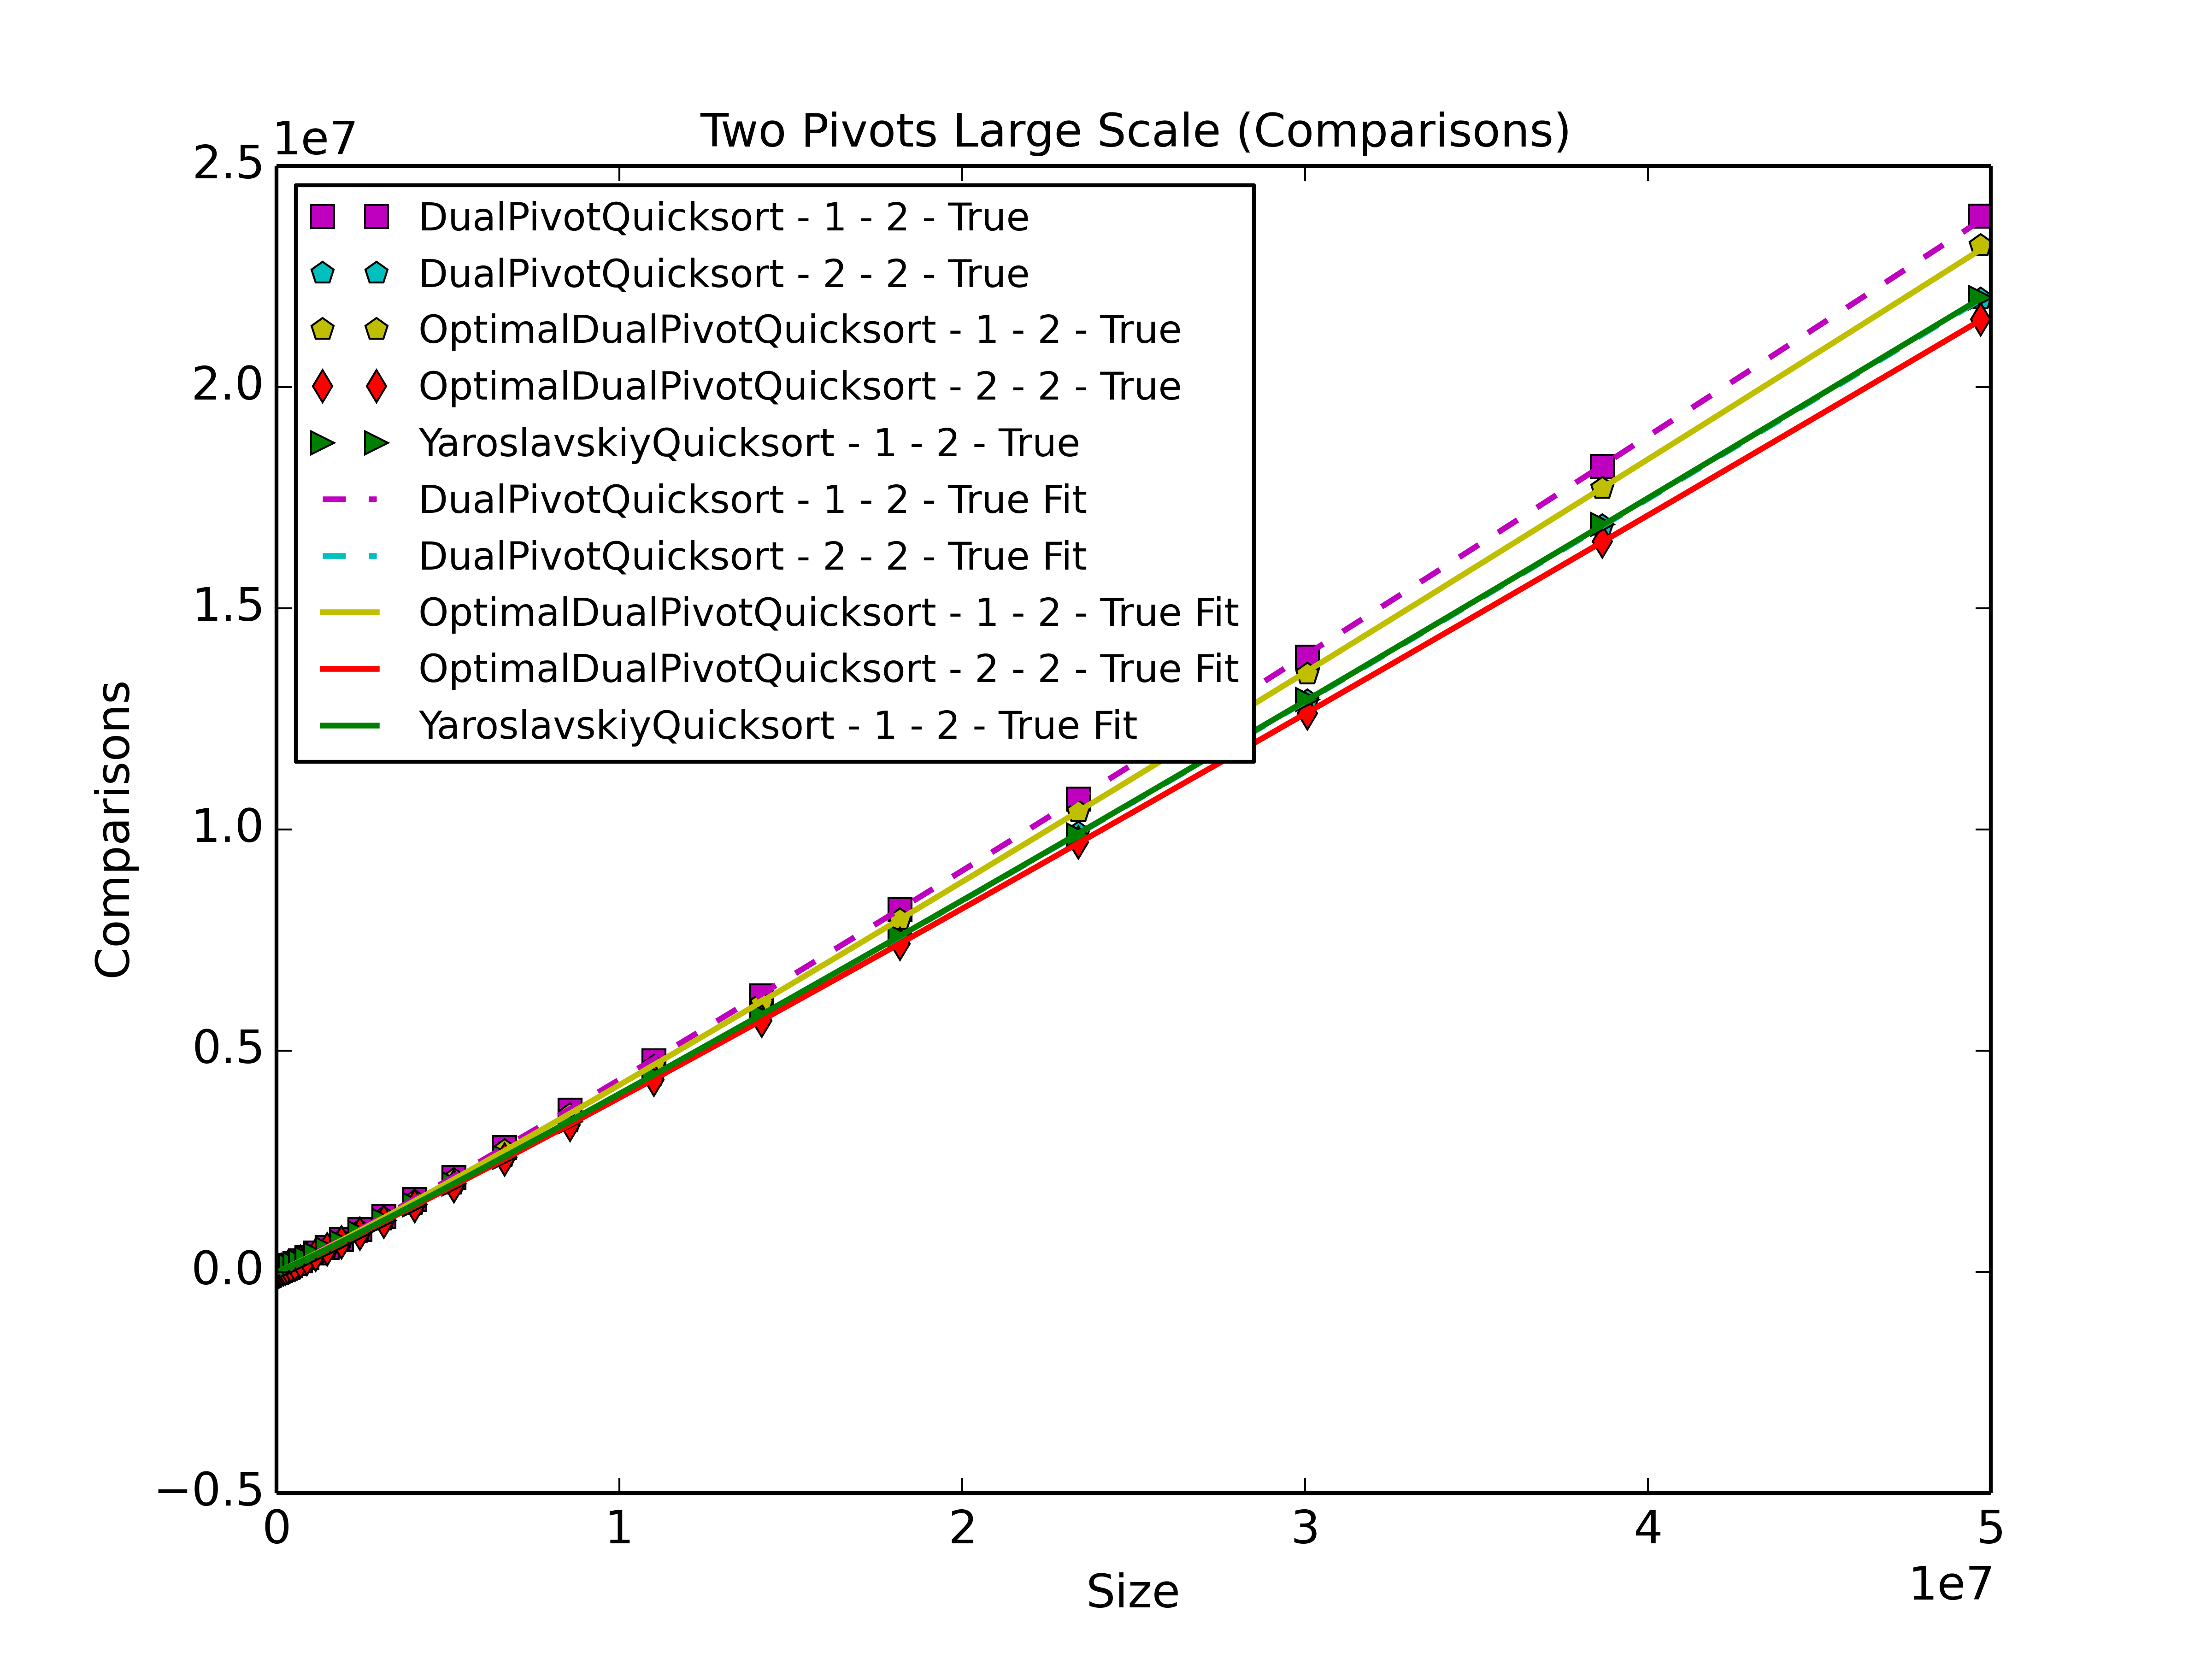
\includegraphics[width=120mm]{TwoPivotsLargeScale_comp.png}
			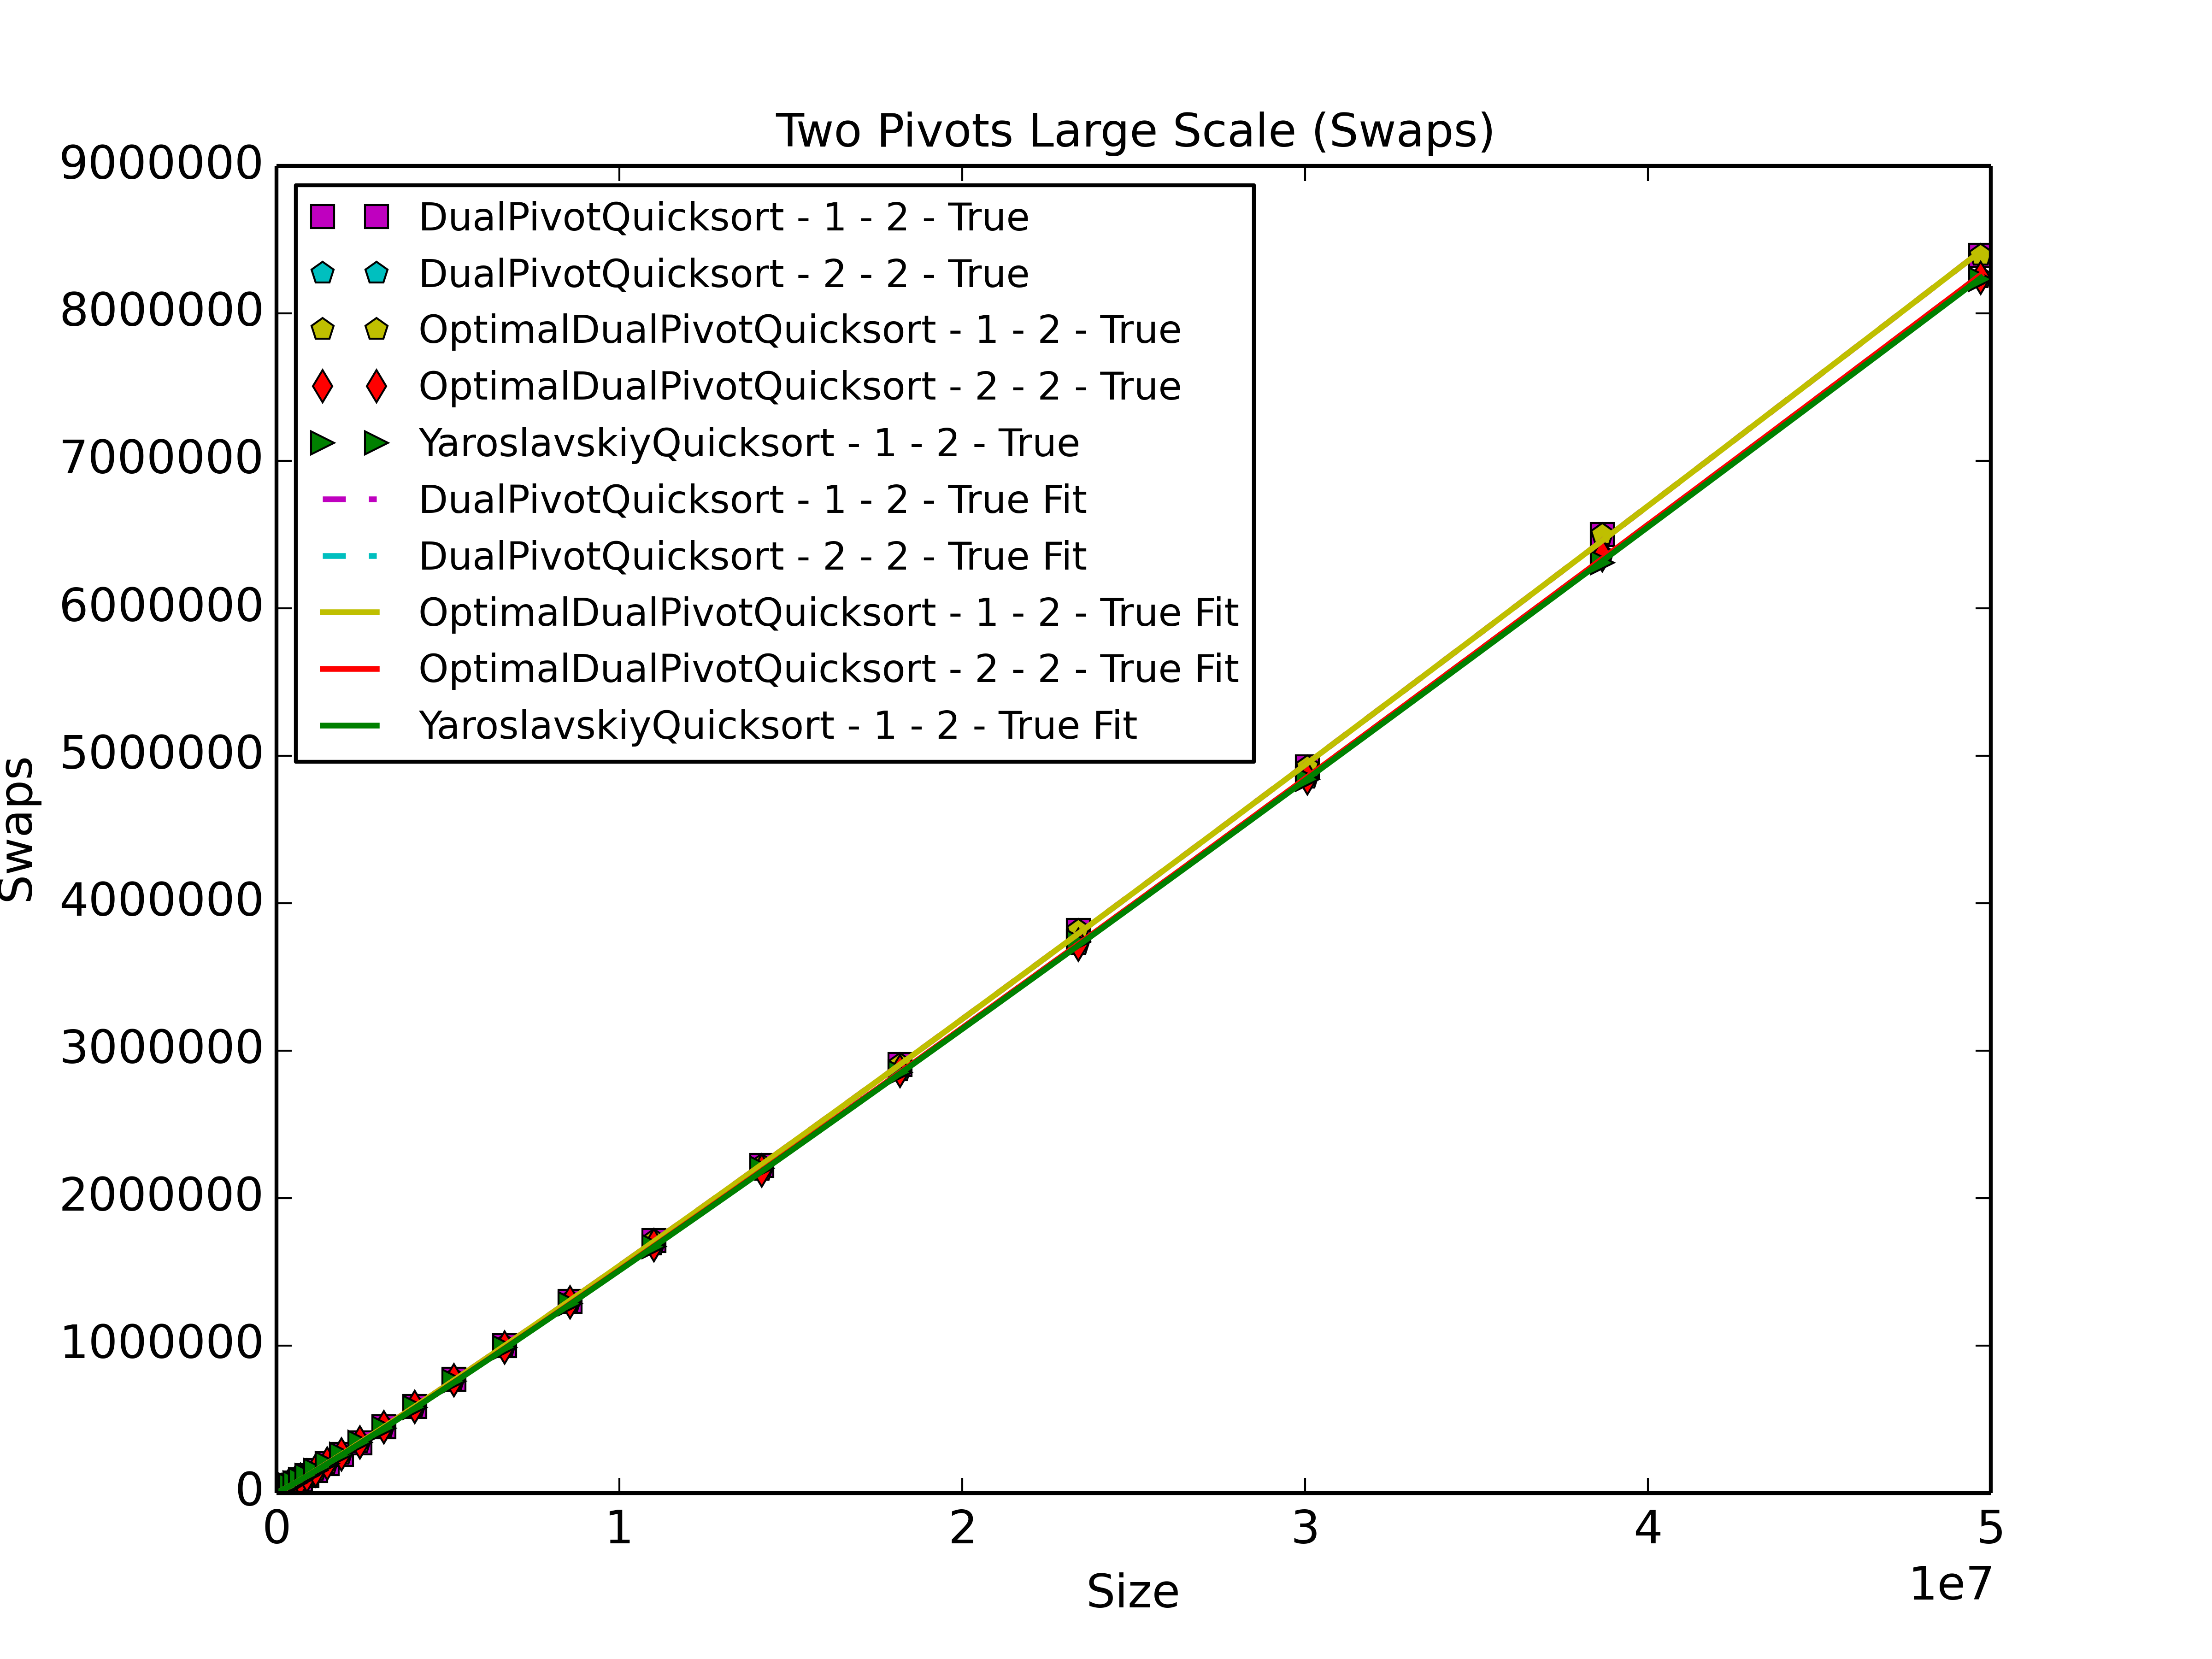
\includegraphics[width=120mm]{TwoPivotsLargeScale_swap.png}
			\caption{A plot of the data from all the sorting algorithm with two pivots}
		\label{fig:TwoPivot}
		\end{center}
	\end{figure}

	%**********************************************************************
	% Three Pivots Large Scale
	%**********************************************************************
	\begin{figure}[ht!]
		\begin{center}
			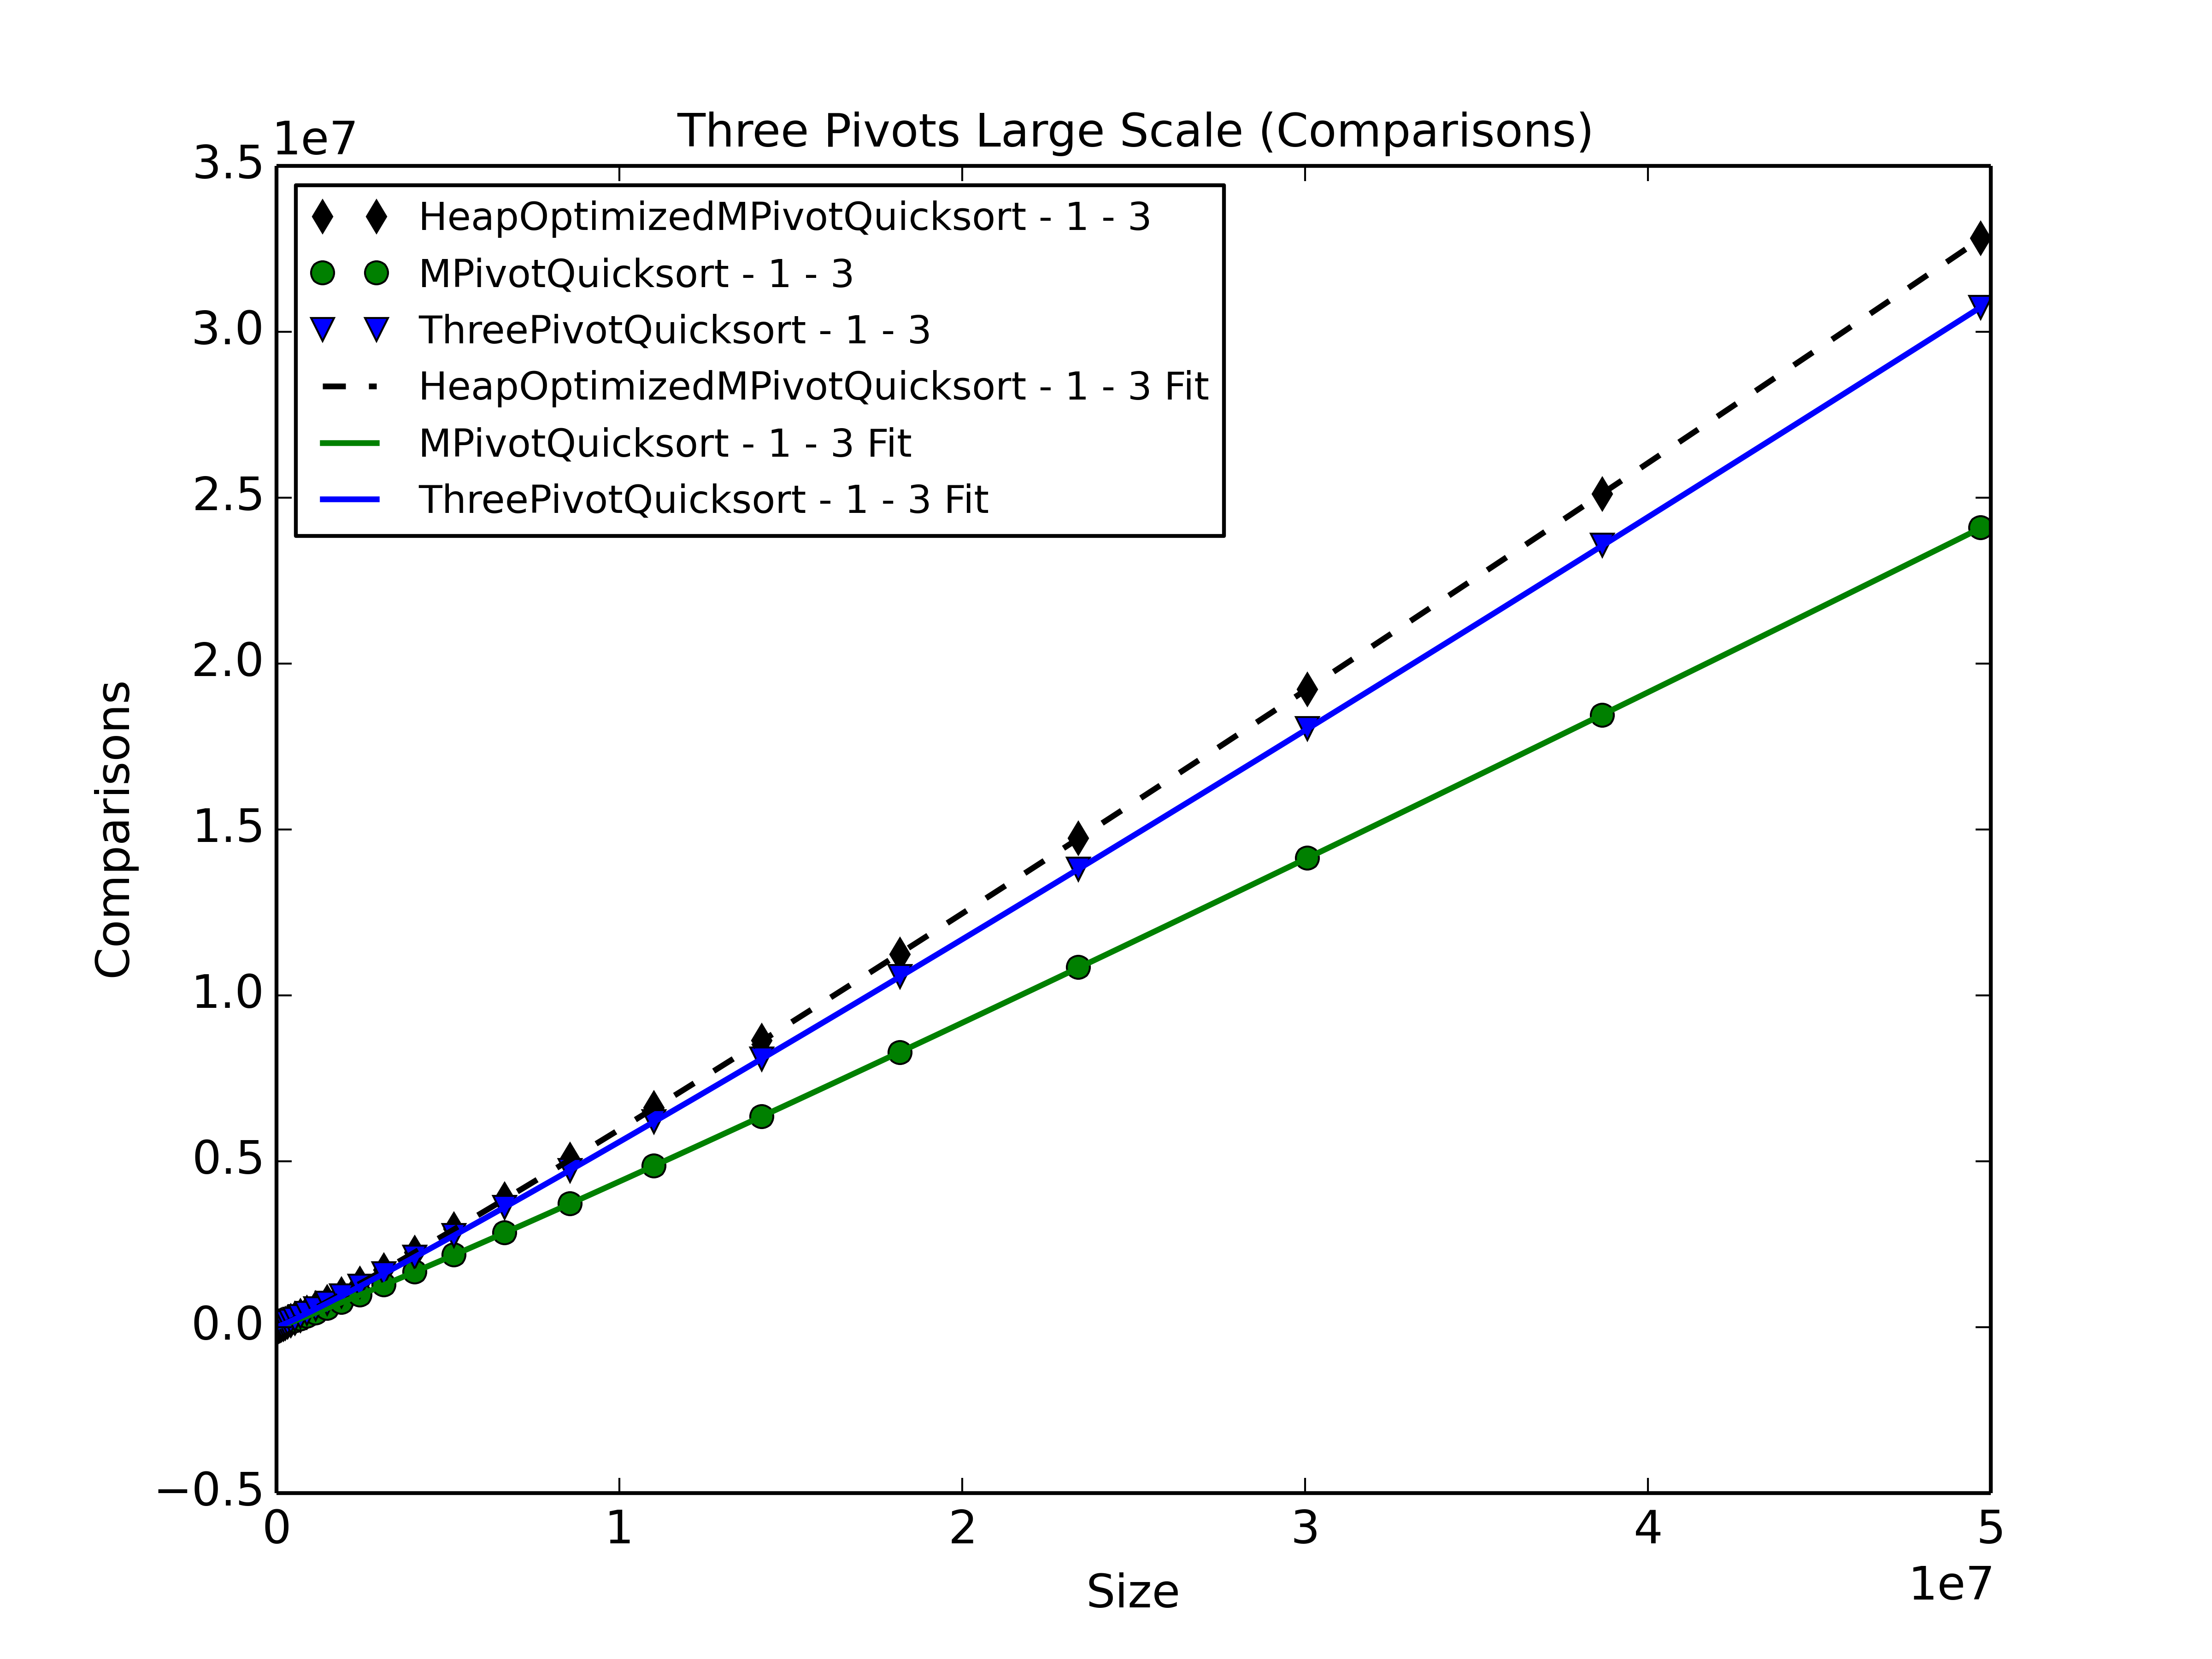
\includegraphics[width=120mm]{ThreePivotsLargeScale_comp.png}
			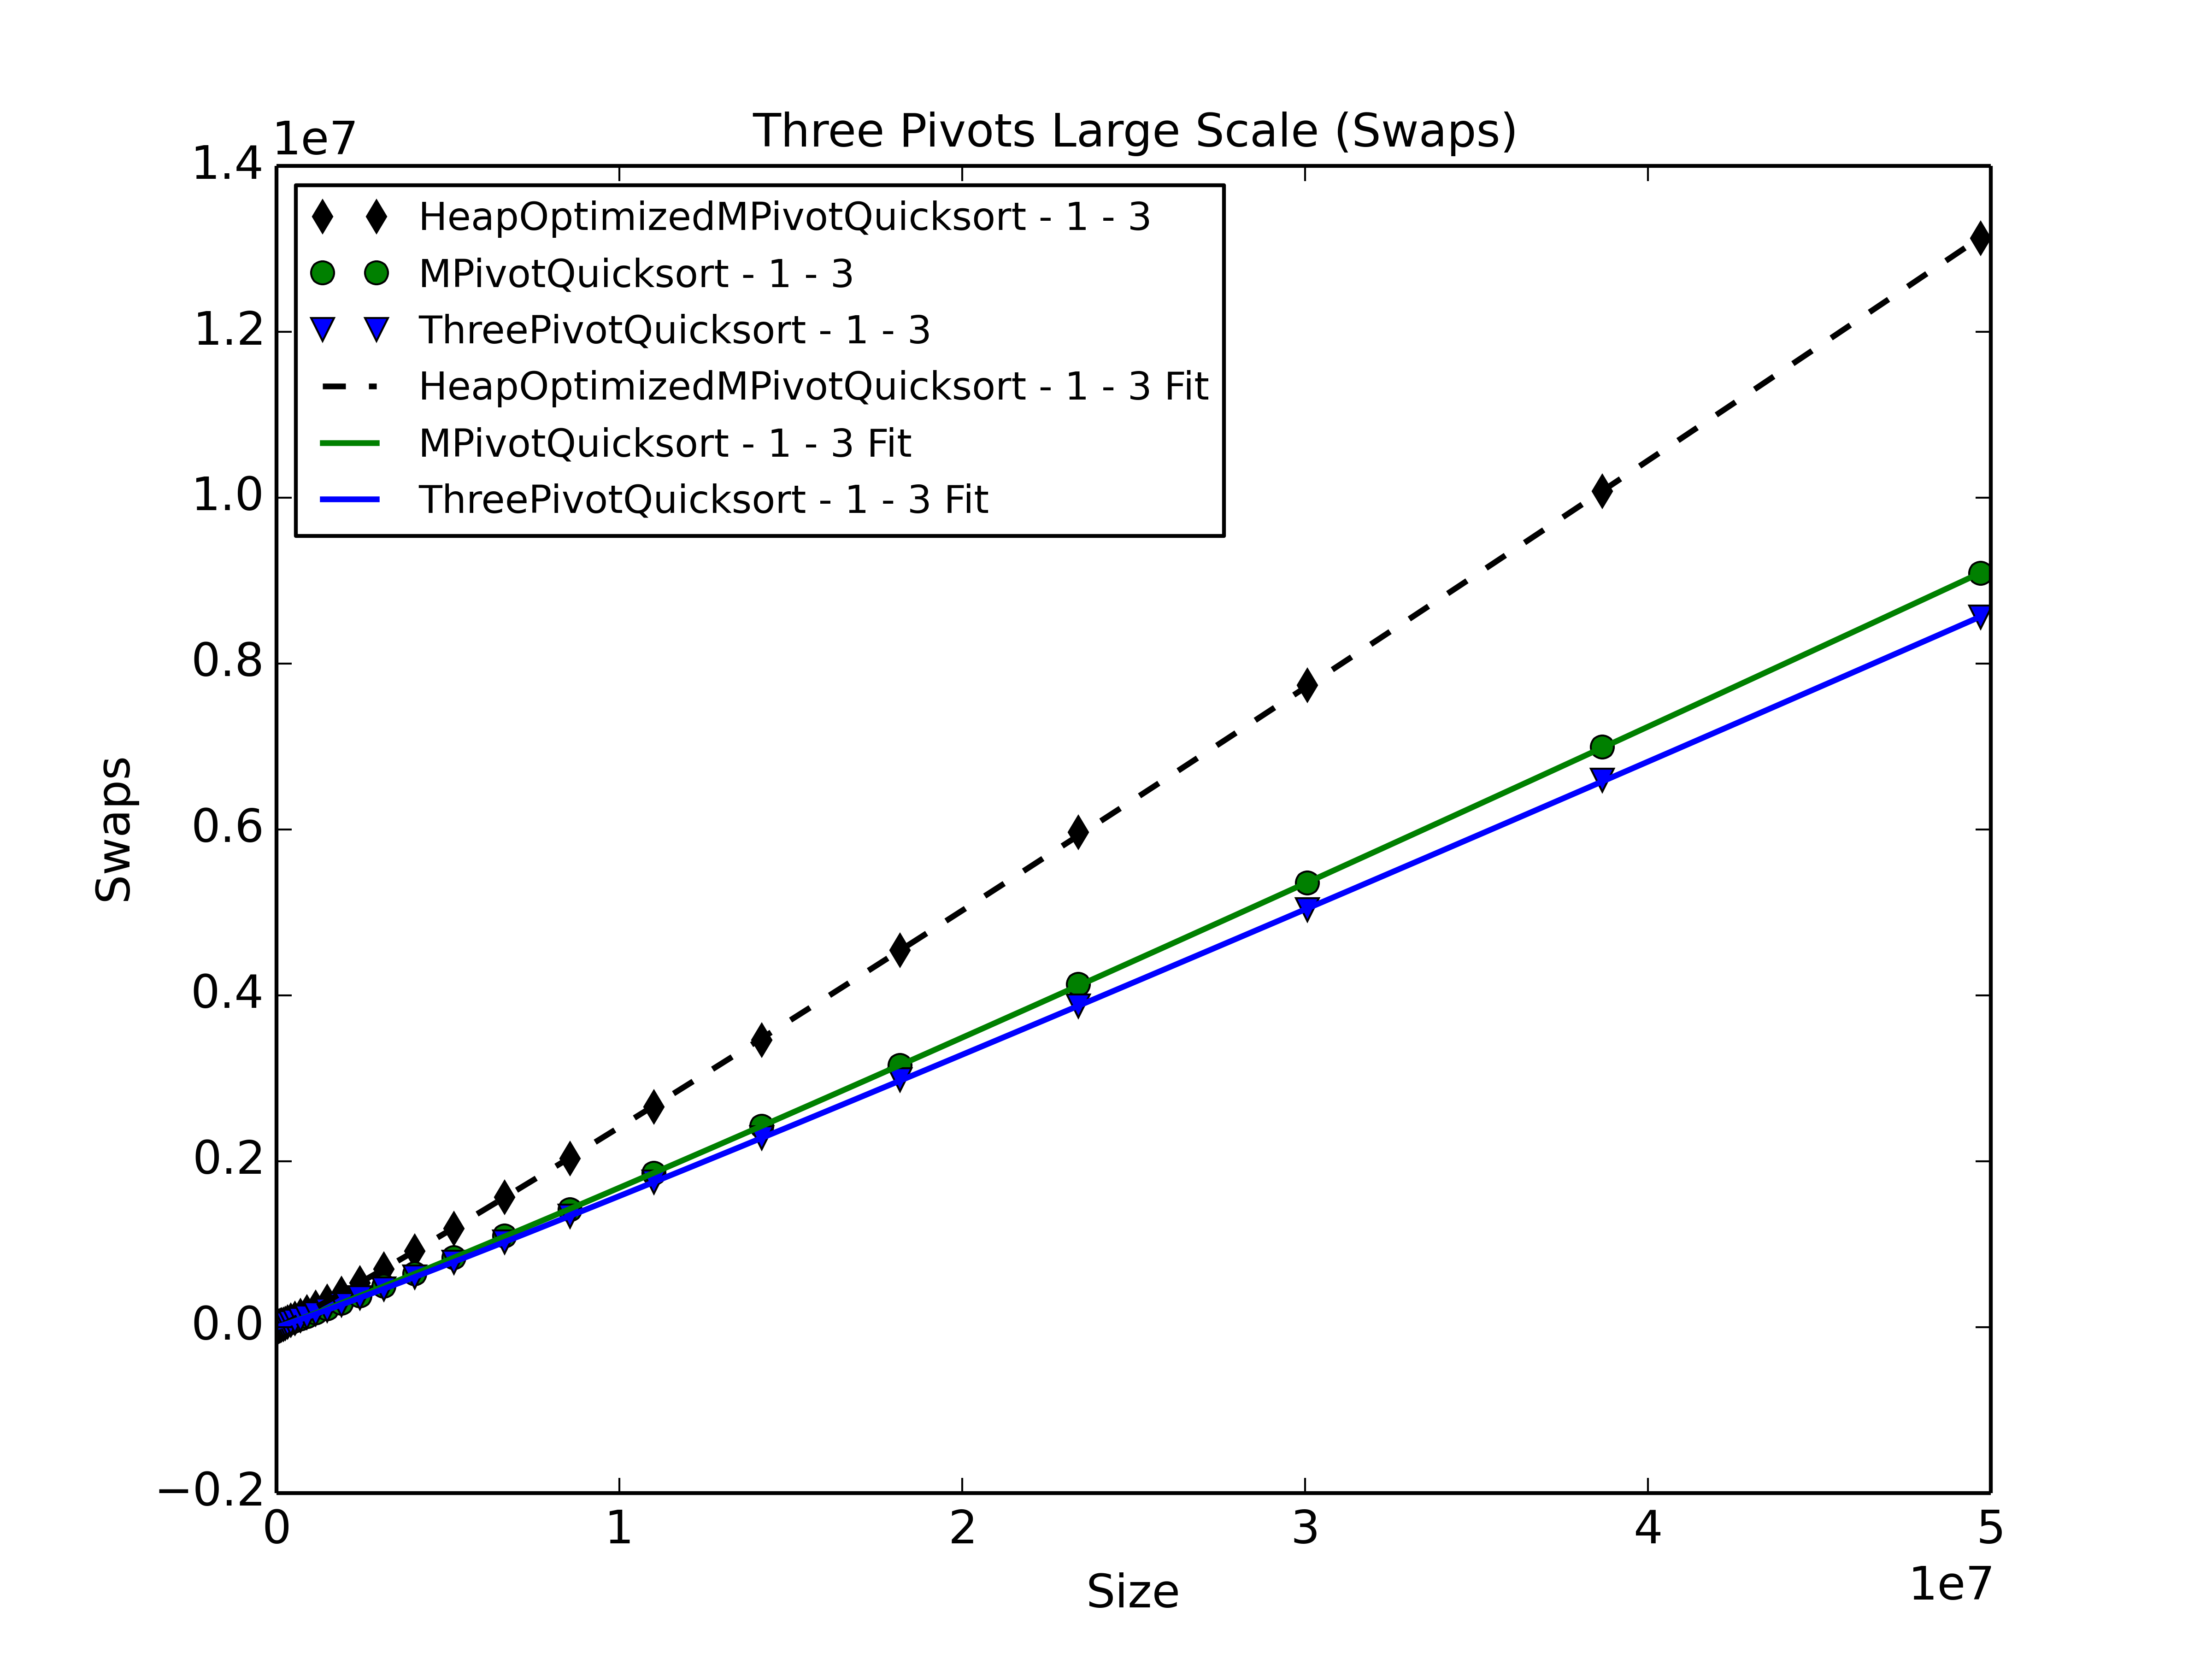
\includegraphics[width=120mm]{ThreePivotsLargeScale_swap.png}
			\caption{A plot of the data from all the sorting algorithm with three pivots}
			\label{fig:ThreePivot}
		\end{center}
	\end{figure}

	%**********************************************************************
	% M-Pivot Pivot Sorts Large Scale
	%**********************************************************************
	\begin{figure}[ht!]
		\begin{center}
			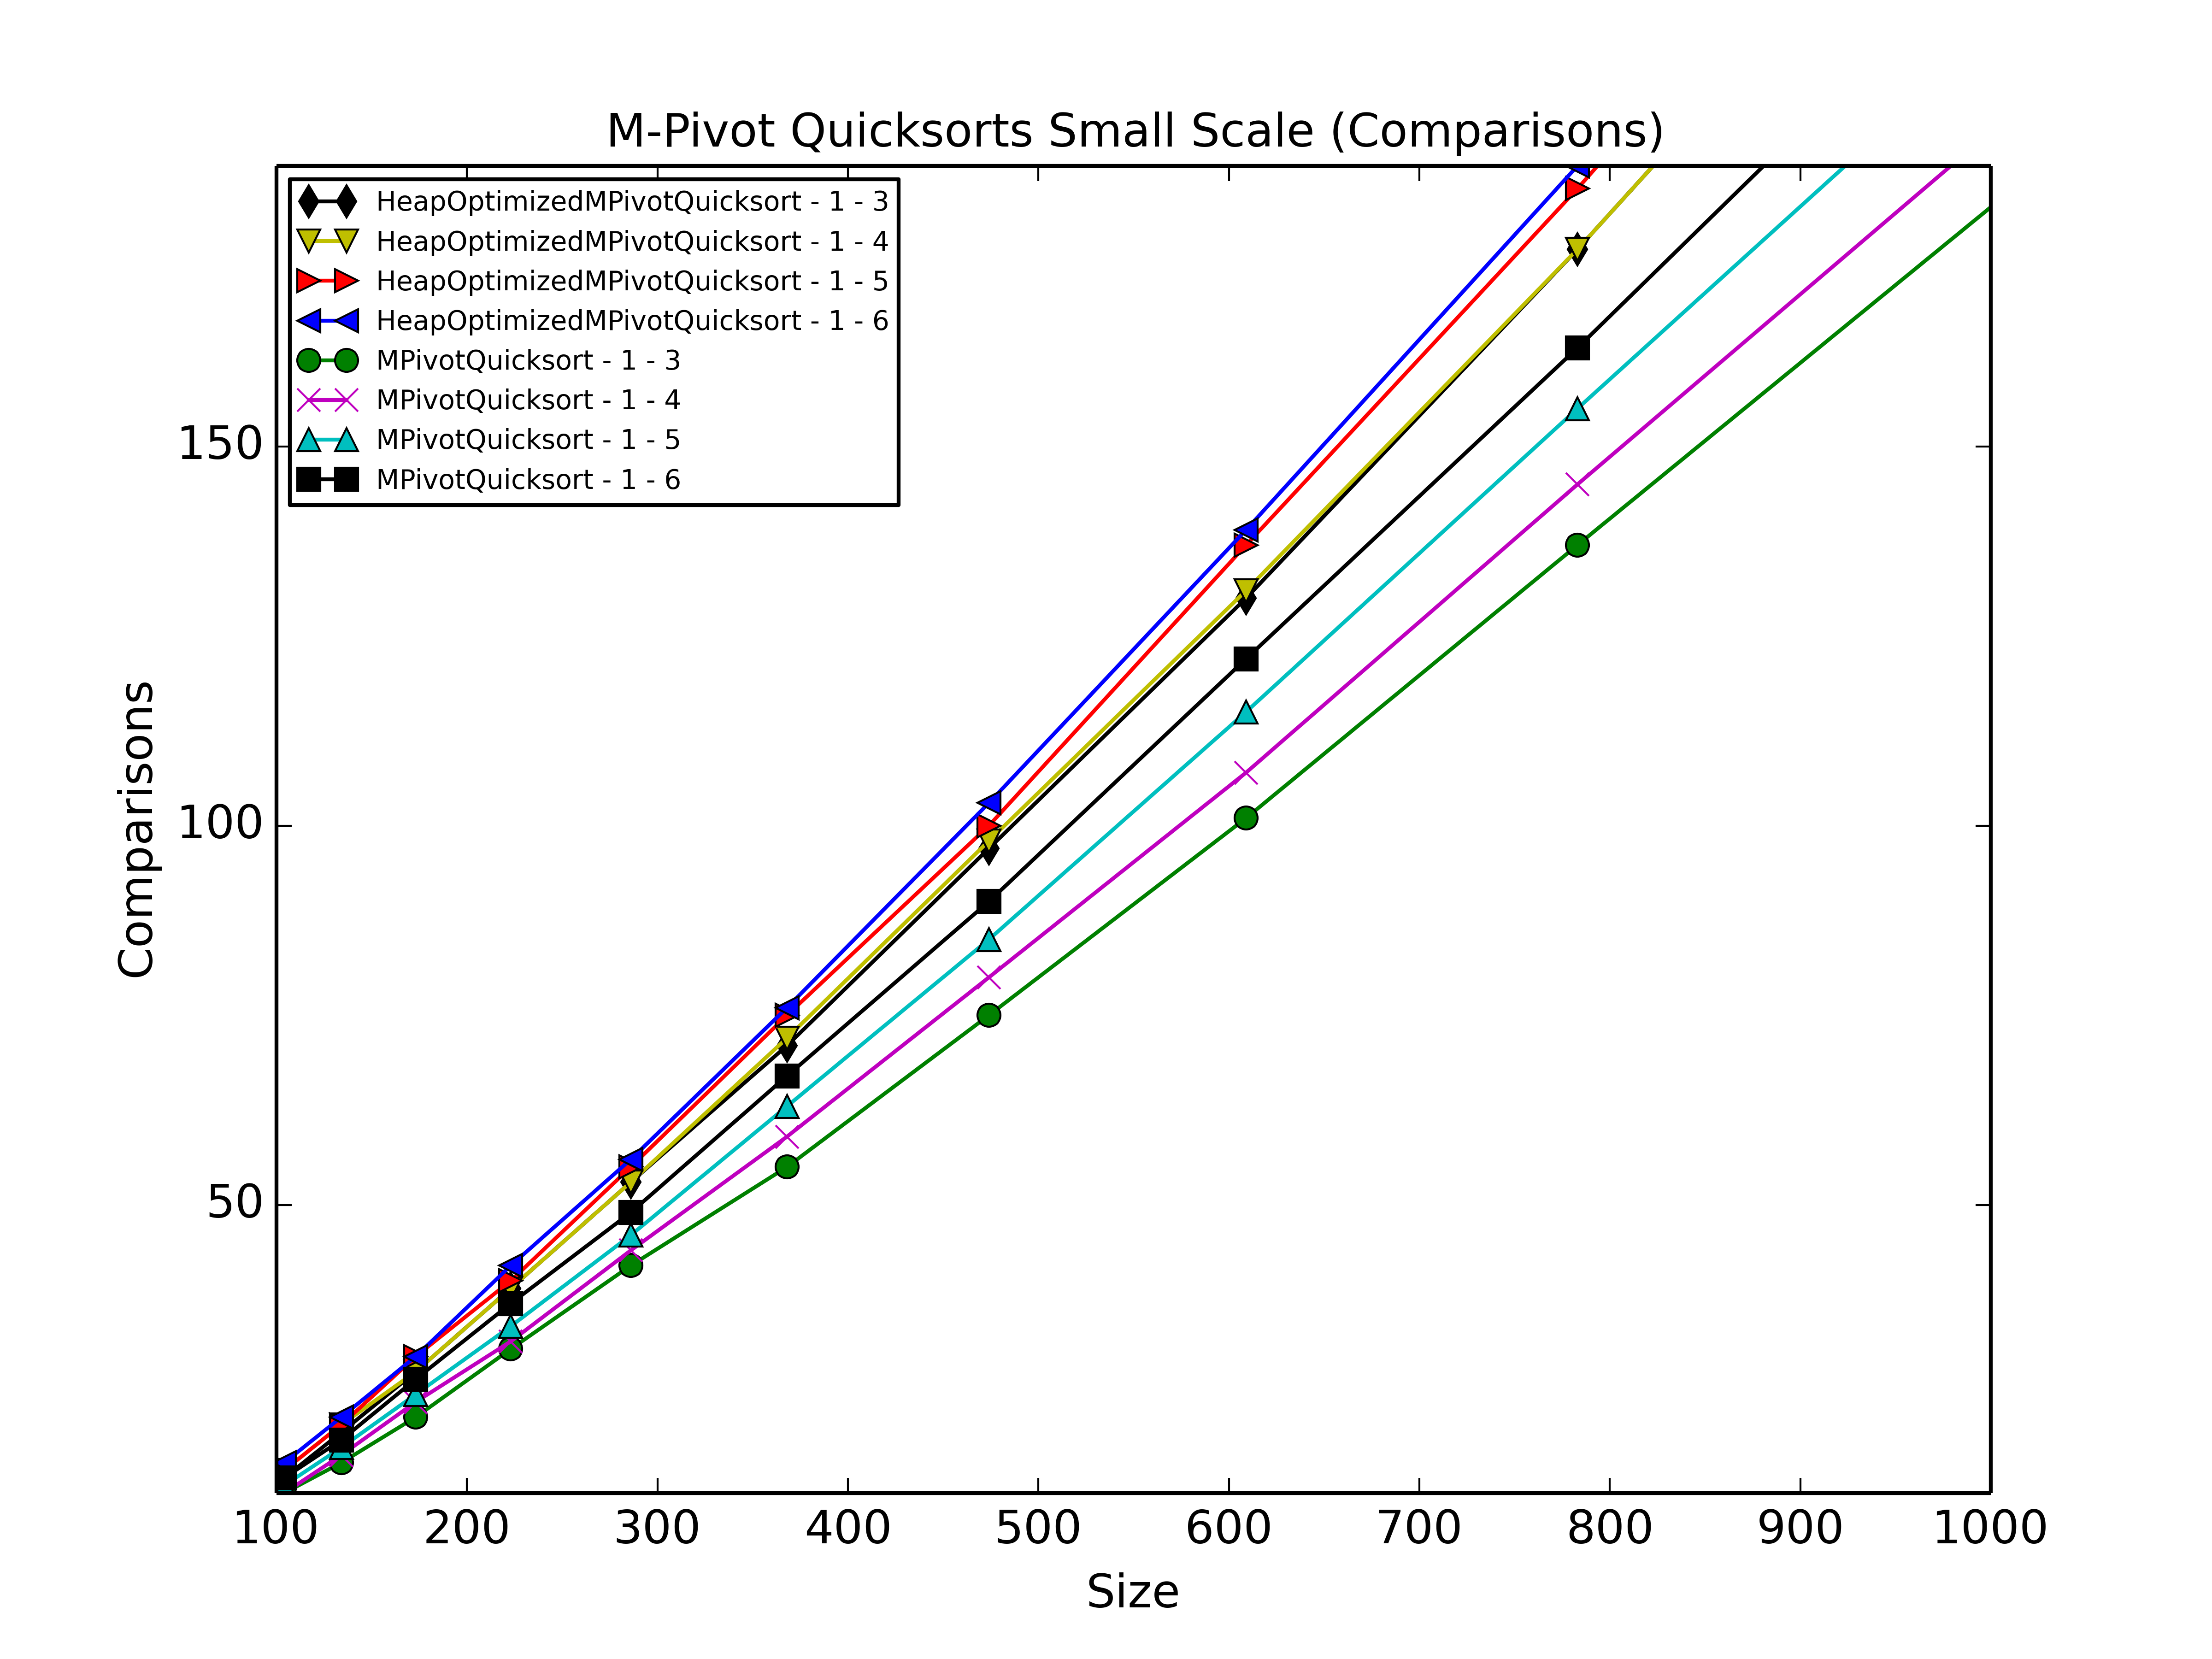
\includegraphics[width=120mm]{M-PivotQuicksortsSmallScale_comp.png}
			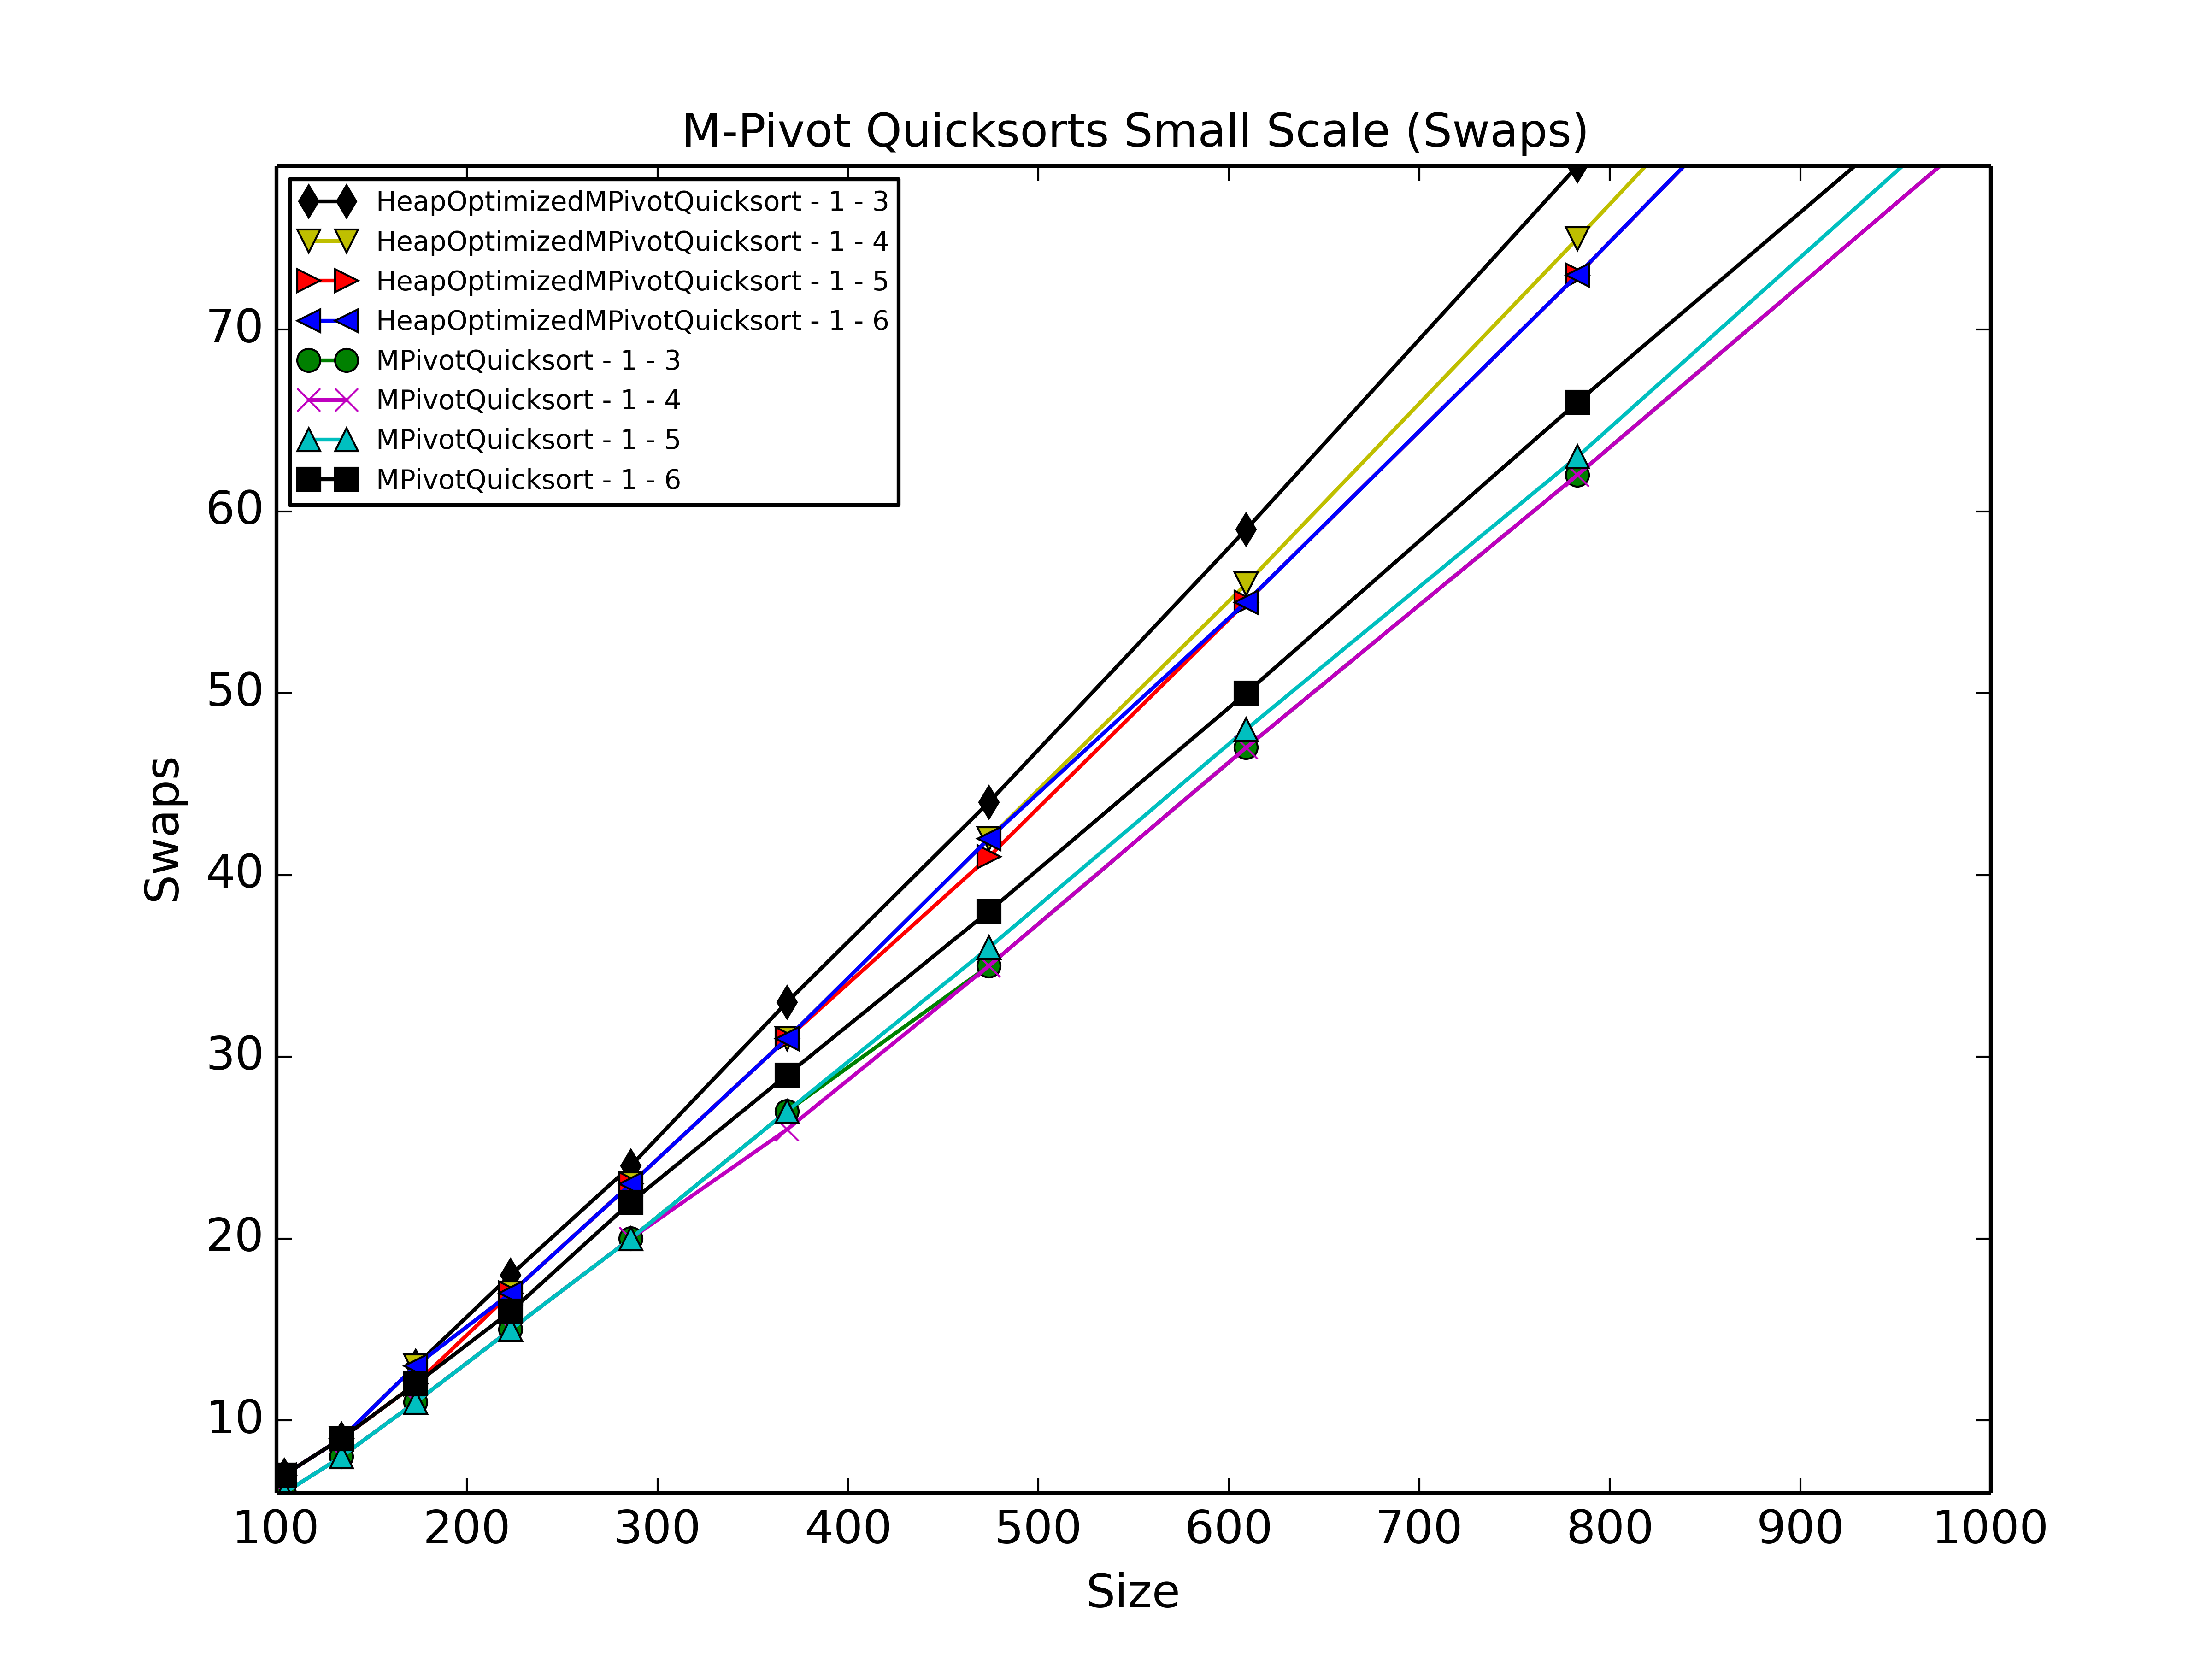
\includegraphics[width=120mm]{M-PivotQuicksortsSmallScale_swap.png}
			\caption{Data from all the version of M-Pivot Sort.}
			\label{fig:MPivot}
		\end{center}
	\end{figure}
